%% main.tex -- GENERATED from gentle-igloo-joas-draft.md by build_tex.py; edit the Markdown.
%% Journal of Open Aviation Science (JOAS) article form. Requires the official class file
%% extra/joas.cls from https://github.com/open-aviation/joas-template (not bundled here).
%% PREVIEW ONLY -- generated by build_tex.py --preview from main.tex. NOT the JOAS layout:
%% the standard article class replaces extra/joas.cls, JOAS front-matter macros are dropped,
%% and biblatex uses the bibtex backend (numeric, unsorted, as in the JOAS class).
\documentclass[11pt,a4paper]{article}
\usepackage[T1]{fontenc}
\usepackage[utf8]{inputenc}
\usepackage{lmodern}
\usepackage[margin=2.3cm]{geometry}
\usepackage{graphicx}
\usepackage{parskip}
\usepackage[font=small,labelfont=bf,labelsep=period]{caption}
\usepackage{csquotes}
\usepackage[backend=bibtex,style=numeric,maxbibnames=10,sorting=none]{biblatex}
\usepackage[hidelinks]{hyperref}
\newcommand{\orcid}[1]{}
\newcommand{\previewaffiliation}{}
\newcommand{\affiliation}[1]{\renewcommand{\previewaffiliation}{#1}}
\newcommand{\previewemail}{}
\newcommand{\email}[1]{\renewcommand{\previewemail}{#1}}
\newcommand{\previewkeywords}{}
\newcommand{\keywords}[1]{\renewcommand{\previewkeywords}{#1}}
\newcommand{\abbreviations}[1]{}
\date{Reading preview generated from \texttt{main.tex}; not the JOAS layout}









\addbibresource{reference.bib}

%% pandoc table/figure support (harmless if the class already loads these)
\usepackage{longtable}
\usepackage{booktabs}
\usepackage{array}
\usepackage{calc}
\usepackage{xcolor}
\usepackage{amsmath}
\providecommand{\tightlist}{\setlength{\itemsep}{0pt}\setlength{\parskip}{0pt}}
\providecommand{\real}[1]{#1}
\providecommand{\passthrough}[1]{#1}
\providecommand{\pandocbounded}[1]{#1}
\newcommand{\placeholder}[1]{\textcolor{red}{[[RESULT:#1]]}}
\graphicspath{{../figures/}}

% --- below is the area for authors ---

% Title within 12 words
\title{A Recording-Regime Mixture for Taxi-Out Time Reconstruction at Ten European Airports}

\author{Denys Kolomiiets \orcid{0000-0000-0000-0000}}  % [[RESULT: ORCID]]
\affiliation{Independent researcher, team gentle-igloo}
\email{correspondence@email.domain}  % [[RESULT: contact e-mail]]

% maximum five keywords
\keywords{taxi-out time; recording regimes; ADS-B surface tracks; gradient boosting; open aviation data}

\abbreviations{
    NM: Network Manager,
    RMSE: root-mean-square error,
    PRC: Performance Review Commission,
    LIRF: Rome Fiumicino airport (ICAO code),
    ADS-B: Automatic Dependent Surveillance--Broadcast
}

\begin{document}
\maketitle
\noindent\textit{\previewaffiliation}\par

%% Draft notice (from the Markdown source; not typeset):
%% \textbf{Draft status.} This manuscript describes the solution as of 10 October 2026: 114 scored submissions on the ordinary leaderboard (111 through 8 October, then two measurement uploads and one control upload on 9 October) and the sealed final file. Every number is copied from the repository documentation (\texttt{README.md}, \texttt{docs/*.md}, \texttt{docs/tables/*.csv}, the dated reports in \texttt{analysis/}, the experiment register \texttt{HYPOTHESES\_LOG.md} up to entry 448). Items marked \texttt{\placeholder{\ \ldots{}}} are the only gaps left: the organiser's blind final ranking after 14 October 2026, the author's ORCID and contact e-mail, and the DOI of a public archive if one is created. The draft is not an accepted article and must not be cited as one. \texttt{paper/OUTLINE.md} lists the evidence behind each section; \texttt{paper/build\_tex.py} turns this file into \texttt{paper/main.tex}.

\begin{abstract}
The EUROCONTROL Performance Review Commission Data Challenge 2026 asked for the recorded taxi-out time of departures at ten European airports: train on 2025, score root-mean-square error (RMSE) on January and July 2026, then a blind four-month final. Team gentle-igloo reached 230.48 s, 16th of 239 teams on 8 October 2026 \placeholder{ final ranking --- blind four-month rank}. The design follows three properties of the data. First, the label is a recorded interval produced by several recording regimes: 6.8 \% of 2025 labels equal take-off minus a planning time within 6 s, and at Rome Fiumicino 83.7 \% of labels above one hour do. A classifier weights a regular-duration estimate against five such candidates and predicts the probability-weighted mean. Second, the Network Manager actual off-block time is a strong but biased anchor (384.9 s RMSE alone); gradient-boosted trees learn the residual to a per-airport calibrated proxy. Third, the aircraft's own ADS-B ground track shows when it started moving and feeds coverage-gated correction stages and a neural member. Temporal month-pair cross-validation with pre-registered rules showed what transfers to the leaderboard: observations of the flight did, learned capacity on 2025 aggregates did not. For the final we removed the two leaderboard-specific parts of the best file and priced each by a single upload (+0.57 s and +0.70 s). The final file's January/July rows then scored 231.18 s, 0.56 s better than the best score plus both prices; a label-free decomposition traced the difference to refitted regime probabilities on about 350 rows, within a noise of $\pm$0.43--0.55 s that our $\pm$0.3 s corridor had underestimated. As a data-quality detector the regime classifier counts substituted records accurately, and an additional-taxi-out indicator computed from the final predictions matches the published June and July 2026 values within 9.2 and 6.6 s on average.
\end{abstract}

\noindent\textbf{Keywords:} \previewkeywords\par

\section{Introduction}\label{introduction}

Taxi-out time, the interval between an aircraft leaving its stand and taking off, is one of the operational quantities that the EUROCONTROL Performance Review Unit (PRU) monitors at European airports. The PRU's \emph{additional taxi-out time} indicator compares the observed taxi-out time with a reference time for the stand and runway used, and reads the difference as an approximate measure of departure-queue time during congested periods \autocite{eurocontrol2023atxot}. The indicator is computed from the Airport Operator Data Flow combined with Network Manager (NM) trajectory data \autocite{eurocontrol2023atxot}. Taxi-out time is therefore both an operational variable and a recorded one: what is monitored is the interval between two recorded timestamps, and the quality of the recording is part of the quantity.

The PRC Data Challenge 2026 \autocite{prc2026site} made this quantity the target of an open modelling competition. Participants received all 2025 departures and arrivals at ten airports (EDDF, EDDM, EGLL, EHAM, LEBL, LEMD, LFPG, LIRF, LSZH, LTFM) with NM flight records, and were asked to predict the recorded taxi-out time \texttt{TAXITIME\_\allowbreak{}SEC\_\allowbreak{}mvt} of 344,841 departures in January and July 2026, scored by RMSE on a public leaderboard with at most five uploads per UTC day. The organiser required GPLv3 source code, documented open external data and reproduction documentation, and announced that a large part of the prize assessment would rest on model design and documentation rather than on the ranking alone \autocite{prc2026site}; the organiser's dated statements are quoted verbatim in the repository. On 8 October 2026 a blind final phase was added because, in the organiser's words, ``the signs of `optimizing for the ranking' are too strong'': one submission for January, February, June and July 2026 (670,790 departures), ranked separately on the initial two months, the two new months and all four, with the design of the model not to change \placeholder{ final ranking --- one sentence on the outcome of the blind ranking}. Previous editions of the challenge, on take-off weight \autocite{spinielli2025atow} and fuel burn \autocite{sun2026fuel}, were followed by solution papers in this journal \autocite{murca2025atow,grigoriou2026fuel,kacar2026fuel}; this paper follows that practice.

An important feature of the task is what remains visible in the ranking file. Only the departure off-block time and the target are hidden; the take-off time, the NM timestamps of the flight (scheduled, initial, latest and estimated off-block, and the minute-rounded actual off-block \texttt{AOBT\_\allowbreak{}3}), the stand, the runway and all arrivals remain visible. The organiser confirmed on 16 September 2026 that ``the rest in the same row and other rows is available to your model'', and on 19 September that ``the model is for post-ops, not for tactical use''. The task is therefore a \textbf{retrospective reconstruction of when the aircraft left the stand}, not a pre-departure forecast. We state this at the outset because it shapes every design decision and bounds every claim.

We also state at the outset what this paper does not claim. The team stood 16th of 239 on the ordinary leaderboard on 8 October 2026, about 17 s behind the third-placed team; the contribution is not the rank. The paper makes five contributions.

\begin{enumerate}
\def\labelenumi{\arabic{enumi}.}
\tightlist
\item
  We document a \emph{recording-regime} phenomenon in the challenge labels: a substantial fraction of recorded off-block times are copies of planning timestamps, concentrated at one airport, and these rows dominate the squared error. Modelling the recording process as a probability mixture was worth more than any learner choice (Section 2.2, Section 5.1), and the same classifier is a calibrated detector of substituted records (Section 5.6).
\item
  We describe a modular chain (Section 3) in which gradient-boosted trees learn the residual to a calibrated NM proxy, coverage-gated stages correct the estimate from the flight's own ADS-B surface track, a neural member reads the ordered track with a weight chosen at chain level on all twelve months of 2025, and a small tabular foundation model handles a sparse tail.
\item
  We describe a uniform recipe for the blind final that removes the two leaderboard-specific parts of the best file, report the price of each part measured by single uploads rather than inferred, and check the final file's January/July rows against a forecast registered before the upload, including what the check taught us about forecast corridors (Sections 3.8, 5.7).
\item
  We report a validation protocol of temporal month-pair folds with pre-registered decision rules, an account of which classes of change transferred from cross-validation to the leaderboard, a label-free identity for blends of scored files and the limit at which it fails, and a disclosure of every design choice that was taken or kept because of a leaderboard result (Sections 4, 6.3).
\item
  We read the model in PRU terms: a calibrated predictive distribution per flight, the effect of substituted records on an emulated additional-taxi-out indicator, a label-free comparison of the final predictions with the indicator EUROCONTROL published for 2026, and a documented set of negative results from the last two days of development (Sections 5.5--5.8).
\end{enumerate}

\section{Data}\label{data}

\subsection{Challenge data}\label{challenge-data}

The training set contains 2,085,047 departures of 2025 at the ten airports, each with the movement record (\texttt{\_\allowbreak{}mvt} columns, sourced from the Airport Operator Data Flow) and, for 98.9 \% of departures, a matched NM flight record (\texttt{\_\allowbreak{}flt} columns) with the scheduled off-block time, the initial, latest and estimated off-block times (IOBT, LOBT, EOBT\_1) and the actual off-block time \texttt{AOBT\_\allowbreak{}3}. The target \texttt{TAXITIME\_\allowbreak{}SEC\_\allowbreak{}mvt} is take-off time minus recorded off-block time. The ranking set holds 344,841 departures of January and July 2026 with the same columns except the hidden off-block time and target. Arrivals are included in both sets with their block times. The final ranking file published on 8 October holds 670,790 departures (January 152,719, February 144,158, June 181,791, July 192,122) and 670,407 arrivals; its timestamps carry a fresh draw of the same $\pm$12 s dithering that every challenge file carries, so the label itself carries noise of up to $\pm$12 s and the regime tolerance of 6 s and the LOBT window of 3,606 s used below are the half-width of that dithering. For a fixed chain the expected effect of a fresh draw on RMSE is zero, with a realised spread of $\pm$0.08 s (1$\sigma$) on January/July; Section 5.7 shows that this does not hold for a refitted chain.

Timestamps are mostly minute-resolved. 97.7 \% of \texttt{AOBT\_\allowbreak{}3} values fall on a whole minute. At EDDM, EGLL, LEBL, LEMD, LFPG, LIRF and LTFM at least 99.95 \% of block times sit within $\pm$6 s of a whole minute; at EDDF, EHAM and LSZH only 21.7--24.9 \% do, close to the 13/60 expected from uniformly distributed seconds, so these three airports record block time to the second. A label at the seven minute-resolved airports is therefore a difference of two minute-resolution times with a few seconds of jitter. Label ranges also differ by airport: LEBL and LEMD labels stop at 3,604 s and 3,598 s, while the other airports reach 6,899--131,167 s; 369 labels are negative.

\subsection{Recording regimes}\label{recording-regimes}

The first property that shaped the model is that the label does not always describe a physical taxi. In 2025, 140,993 labels (6.76 \%) equal take-off minus the scheduled time, IOBT, LOBT or EOBT\_1 within $\pm$6 s, or lie between one day and one day plus two hours after a planning time (a one-day shift). We call these \emph{recording regimes}: the recorded off-block time is a copy of a planning timestamp rather than an observation. Figure~\ref{fig:1} shows the shares per airport.

\begin{figure}
\centering
\pandocbounded{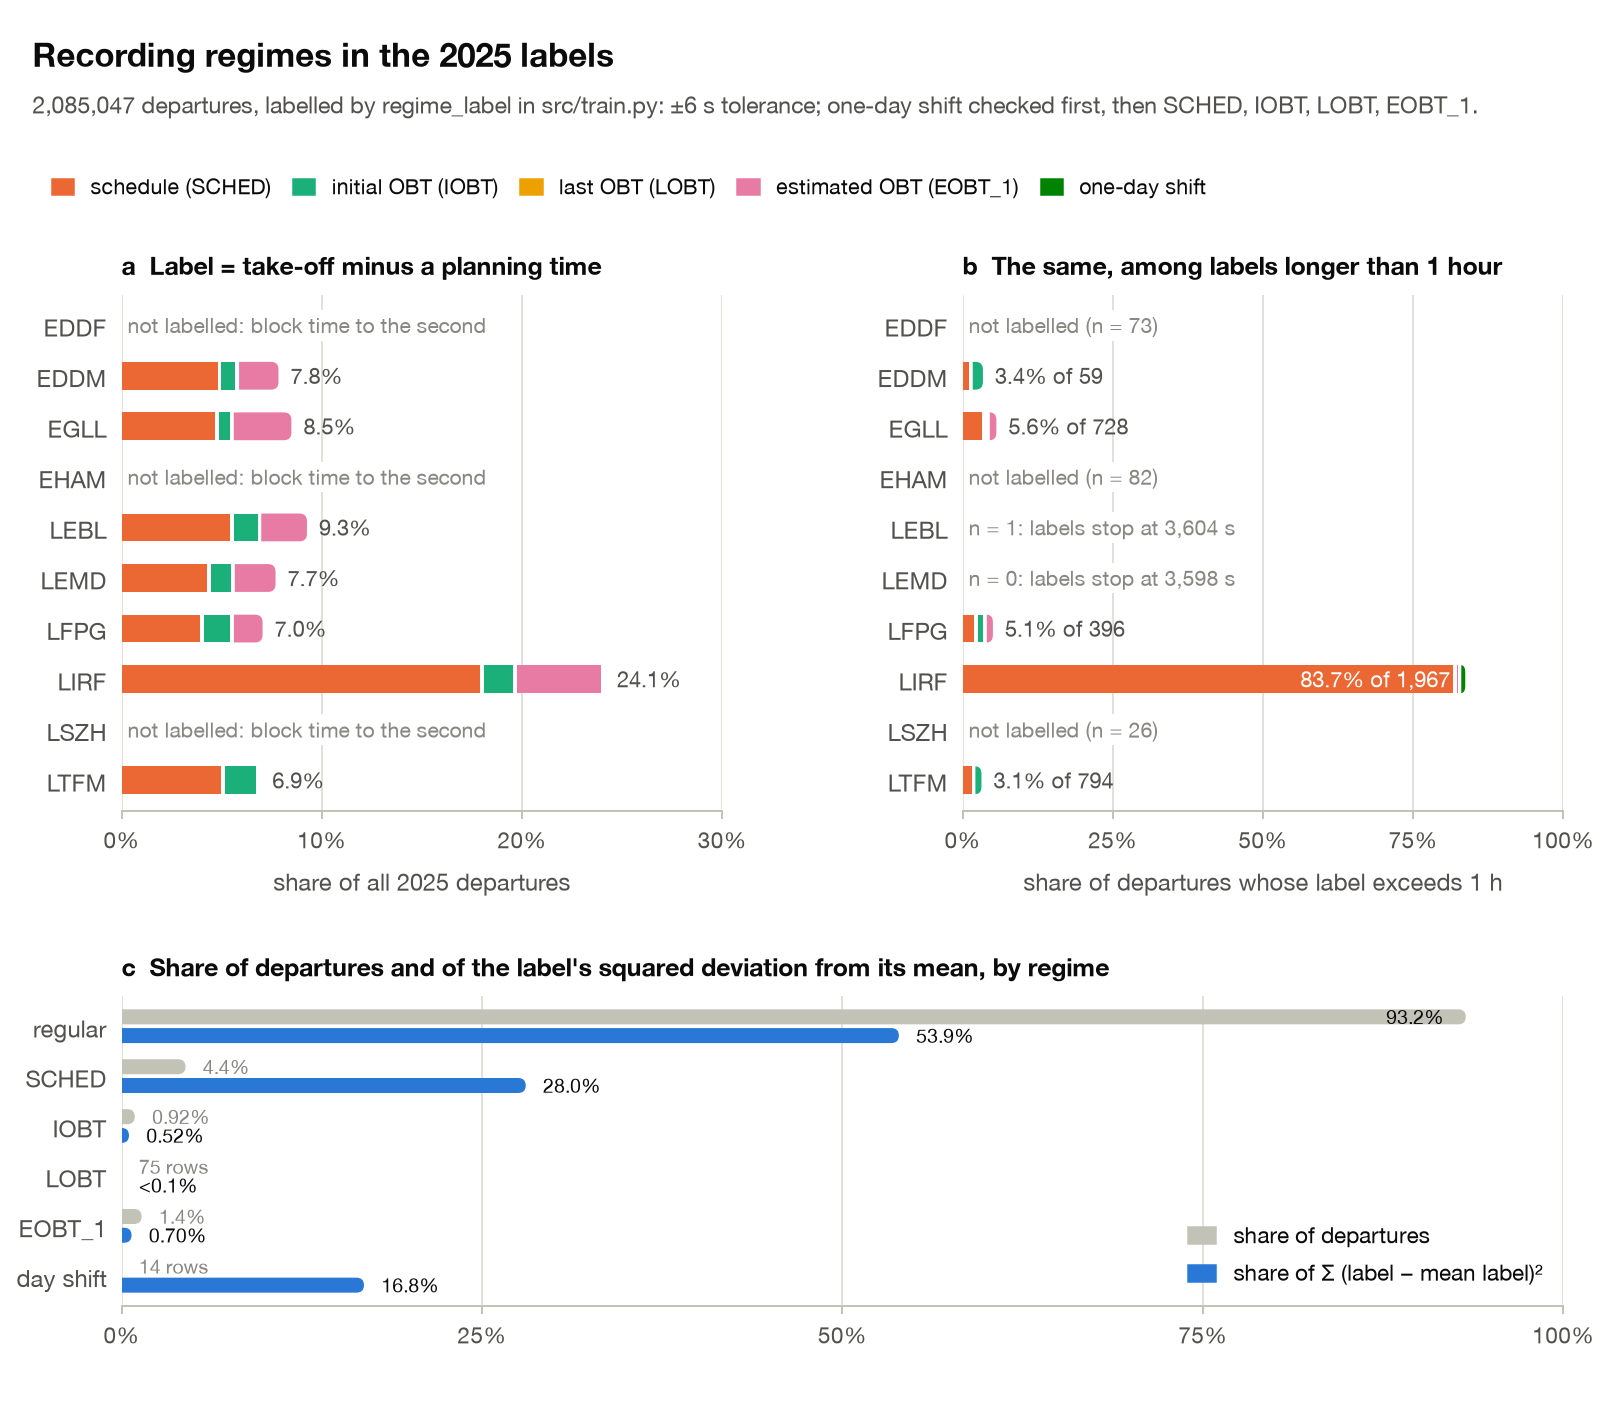
\includegraphics[width=\textwidth]{fig2_recording_regimes.png}}
\caption{Recording regimes in the 2025 labels. (a) Per airport, share of labels equal to take-off minus a planning time (LIRF 24.1 \%; 6.9--9.3 \% at the other six labelled airports). (b) Among labels above one hour, 83.7 \% at LIRF match a planning time against 3.1--5.6 \% elsewhere. (c) The schedule class is 4.4 \% of rows but 28.0 \% of the label's squared deviation from its mean; the 14 one-day-shift labels hold 16.8 \%.}\label{fig:1}
\end{figure}

Two tests separate substitution from coincidence. First, a same-minute test: at LIRF 18.1 \% of block times fall in the scheduled minute, against 3.7 \% in the minute before and 1.3 \% in the minute after. At EDDM, EGLL, LEBL, LEMD, LFPG and LTFM the scheduled minute holds 4.1--5.6 \% against 3.5--5.3 \% in its neighbours, which is consistent with on-time pushbacks whose planning-time candidate equals the physical taxi time anyway. Second, the long-label test: among the 1,967 LIRF labels above one hour, 83.7 \% match a planning time, against 3.1--5.6 \% at the other airports with at least 20 such labels. EDDF, EHAM and LSZH, which record block time to the second, show no planned-regime labels and are excluded from regime labelling in the model.

Panel (c) shows why this matters for RMSE. The schedule class is 4.4 \% of rows but holds 28.0 \% of the squared deviation of the label from its mean; 14 one-day-shift labels hold a further 16.8 \%. In January and July 2025, 45 of 344,419 labels exceed four hours and hold 52.4 \% of the label's sum of squared deviations. A single regressor trained on the physical taxi fails exactly where the metric is decided.

The regime labels used for training come from explicit comparisons with the target (\texttt{regime\_\allowbreak{}label} in \texttt{src/\allowbreak{}train.py}): $\pm$6 s tolerance, six classes (regular, schedule, IOBT, LOBT, EOBT, one-day shift), no planned regimes at EDDF, EHAM and LSZH. These are dataset-specific heuristics; they must be reassessed for another source of movement records. The rule is a rule, not ground truth: an on-time departure whose physical off-block falls in the scheduled minute is labelled a copy although nothing was copied, and the same-minute test above says that outside LIRF most labelled rows are coincidences of this kind.

\subsection{The NM off-block proxy}\label{the-nm-off-block-proxy}

The second property is that the NM actual off-block time \texttt{AOBT\_\allowbreak{}3} is a strong but noisy anchor (Figure~\ref{fig:2}). It is present for 98.92 \% of 2025 departures and rounded to the minute. Used directly, take-off minus \texttt{AOBT\_\allowbreak{}3} gives an RMSE of 384.9 s against the label, where a constant prediction gives 546.4 s. Of all proxy errors, 39.4 \% are within two minutes and 74.6 \% within five. The error has an airport-specific offset: the median is $-$118 s at LIRF, +87 s at EDDF, +107 s at EHAM and +296 s at LTFM, where only 16.9 \% of departures are within two minutes. The median absolute error is 121--184 s at nine airports and 356 s at LTFM. On all 2,062,577 departures of 2025 with a LOBT, the recorded block time lies within 3,606 s of the LOBT, which defines a feasibility window used throughout the chain.

\begin{figure}
\centering
\pandocbounded{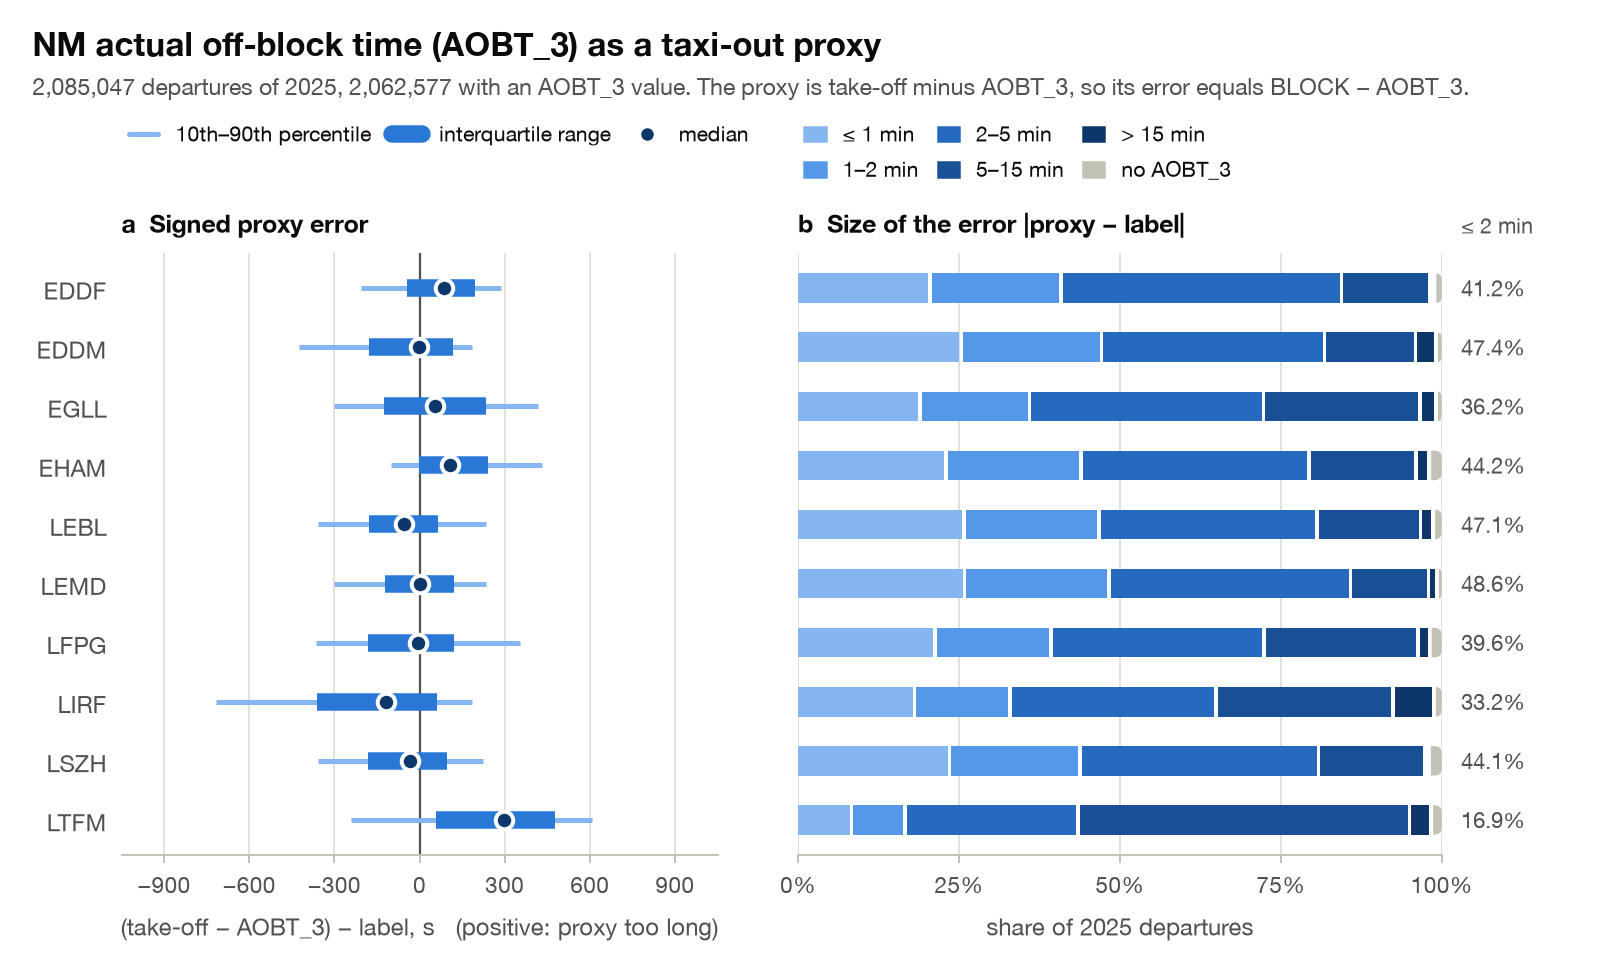
\includegraphics[width=\textwidth]{fig3_nm_proxy_error.png}}
\caption{Signed error of take-off minus AOBT\_3 as a taxi-out estimate, per airport (medians from $-$118 s at LIRF to +296 s at LTFM) and the share of departures by error size (16.9 \% within two minutes at LTFM, 33--49 \% elsewhere).}\label{fig:2}
\end{figure}

Departures without an NM match are 1.08 \% of 2025 rows (1.56 \% in January and July 2025) and 1.53 \% of the ranking set, reaching 4.96 \% at EHAM in January 2026. They have no \texttt{AOBT\_\allowbreak{}3}, LOBT, IOBT or EOBT\_1. In out-of-fold predictions these rows hold 36.6 \% of the squared error (Section 2.6). In the four final months the share is 1.6 / 0.9 / 1.4 / 1.5 \% against 0.9 / 0.8 / 1.4 / 2.1 \% in the same months of 2025; only EHAM January (5.0 \%, 805 rows) and LSZH January (3.0 \%, 300 rows) exceed every 2025 month of their airport.

\subsection{ADS-B surface coverage and its drift}\label{ads-b-surface-coverage-and-its-drift}

The third property is that the aircraft's own ADS-B ground track shows when it actually started moving, but coverage is uneven and changed between the training and ranking months (Figure~\ref{fig:3}). We used the adsb.lol \texttt{globe\_\allowbreak{}history} archives for 2025 and 2026, published under ODbL 1.0 \autocite{adsblol2025,adsblol2026}; the organiser confirmed on 17 September 2026 that this source ``can be considered open data for the challenge''. An \emph{own surface track} means that the departing aircraft has an adsb.lol surface segment before take-off (coverage class $\ge$ 2 in our extraction).

\begin{figure}
\centering
\pandocbounded{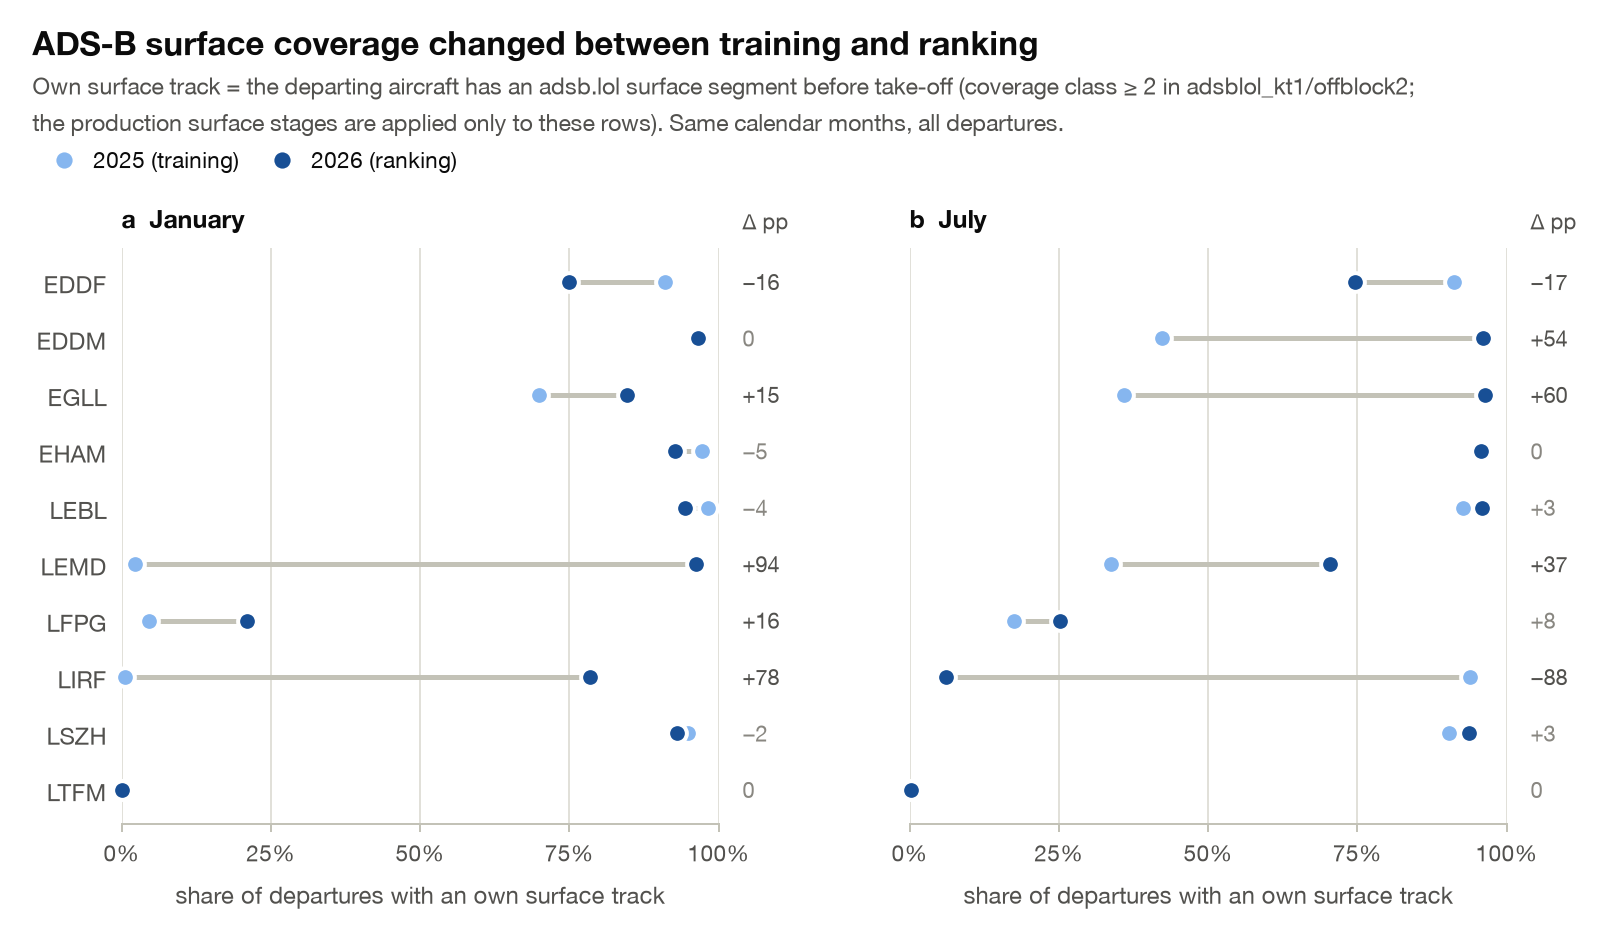
\includegraphics[width=\textwidth]{fig4_adsb_coverage_drift.png}}
\caption{Share of departures with an own ADS-B surface track in January and July, 2025 against 2026, per airport. LIRF goes from 0.6 \% to 78.5 \% in January and from 93.9 \% to 6.2 \% in July; LEMD January from 2.3 \% to 96.3 \%; EGLL July from 35.9 \% to 96.3 \%; LTFM stays near zero.}\label{fig:3}
\end{figure}

Over January and July the share of departures with a track rises from 53.8 \% in 2025 to 64.9 \% in 2026, but single airport-months move much more: LIRF from 0.6 \% to 78.5 \% in January and from 93.9 \% to 6.2 \% in July; LEMD January from 2.3 \% to 96.3 \%; EGLL July from 35.9 \% to 96.3 \%; EDDF down by 16--17 points in both months. LTFM has practically no surface track in either year and LFPG stays between 5 \% and 25 \%. A model that learned \emph{where aircraft are heard}, rather than \emph{how they move}, would not transfer. This drove the decision to use ADS-B as coverage-gated correction stages rather than as base features (Section 3.5), and to drop reception-density features whose behaviour did not transfer.

The two months added for the blind final continue the pattern. Seven daily surface products were rebuilt for all 120 final days from the archives with the final movement times; the share of departures with an own surface segment is 67.6 / 63.8 / 64.0 / 62.9 \% in January / February / June / July 2026 against 50.3 / 51.8 / 64.0 / 55.9 \% in the same months of 2025, but three airport-months collapse: EDDF February 2026 at 32.2 \% against 96.3 \% in 2025 (every day at 15--46 \%, aircraft seen airborne for 92--98 \% of departures but the ground segment not received), LIRF June 2026 at 0.7 \% against 80.3 \%, and LIRF July at 6.2 \% against 93.9 \%. LEMD January/February rose to 96--97 \% from 0--2 \%, EGLL June/July to 93--96 \% from 34--36 \%. One archive day, 11 June 2026, is defective at the source (91,473 points against a median of 1.24 million; both replicas truncated) and is processed as it is. Where the track is missing the stages leave the base prediction unchanged (Section 3.5).

An early probe of adsb.lol on 13 September 2026 concluded that there was no ground coverage; it had read ground state only from the \texttt{ground} flag, which is set on 0.02 \% of points at EDDM. The source was reopened on 15 September after a public competitor reported a gain from the same archive. We record this because a rejection depends on the measurement used (Section 4.3).

\subsection{Other external data}\label{other-external-data}

The remaining external inputs are OpenStreetMap stand, runway and taxiway geometry (ODbL 1.0, retrieved through Overpass) \autocite{osm}; the Iowa Environmental Mesonet METAR archive (public domain per the IEM statement) \autocite{iem}; daily arrival ATFM delay per destination airport from the EUROCONTROL Aviation Intelligence Portal (portal terms: free with attribution, non-commercial; accepted as open data for the challenge by the organiser on 17 September 2026); and Open Performance Data Initiative (OPDI) v0.0.2 exit-parking and taxiway events \autocite{opdi}, used for a correction at LSZH only (accepted as open by the organiser on 4 October 2026). The TabPFN-2 classifier weights are used under the Prior Labs License 1.1 and are not redistributed. The challenge data themselves are provided by the organiser to all teams and are not redistributed. Section 7 lists each source with its terms; the organiser's statements are quoted with timestamps in the repository. One input was considered and refused on licence grounds: Schiphol's announcement of taxiway works in June 2026 carries no open licence, and under the organiser's rule (``if no open license is present it is not open'') it is context for Section 6.2, not a model input.

\subsection{Error budget}\label{error-budget}

Figure~\ref{fig:4} decomposes the 2025 out-of-fold squared error of the chain before its final blend (E195 \texttt{joint} arm, 2,084,921 rows, RMSE 218.3 s; Section 4.1 defines the out-of-fold predictions). LIRF holds 7.7 \% of rows and 30.8 \% of the squared error, LFPG 11.5 \% and 21.6 \%. EDDF, EDDM and EHAM together hold 31.0 \% of rows and 6.5 \% of the error. Three one-day-shift rows hold 13.5 \%, and 11 labels above four hours hold 25.4 \%. The 1.07 \% of rows without an NM record hold 36.6 \%. Rows without an own surface track are 39.5 \% of the data, hold 57.1 \% of the error and have an RMSE of 262.3 s against 183.8 s with a track (229.2 s against 145.4 s on labels up to 7,200 s). The ten largest errors make up 25.8 \% of the total and the largest 1 \% of rows 62.0 \%.

\begin{figure}
\centering
\pandocbounded{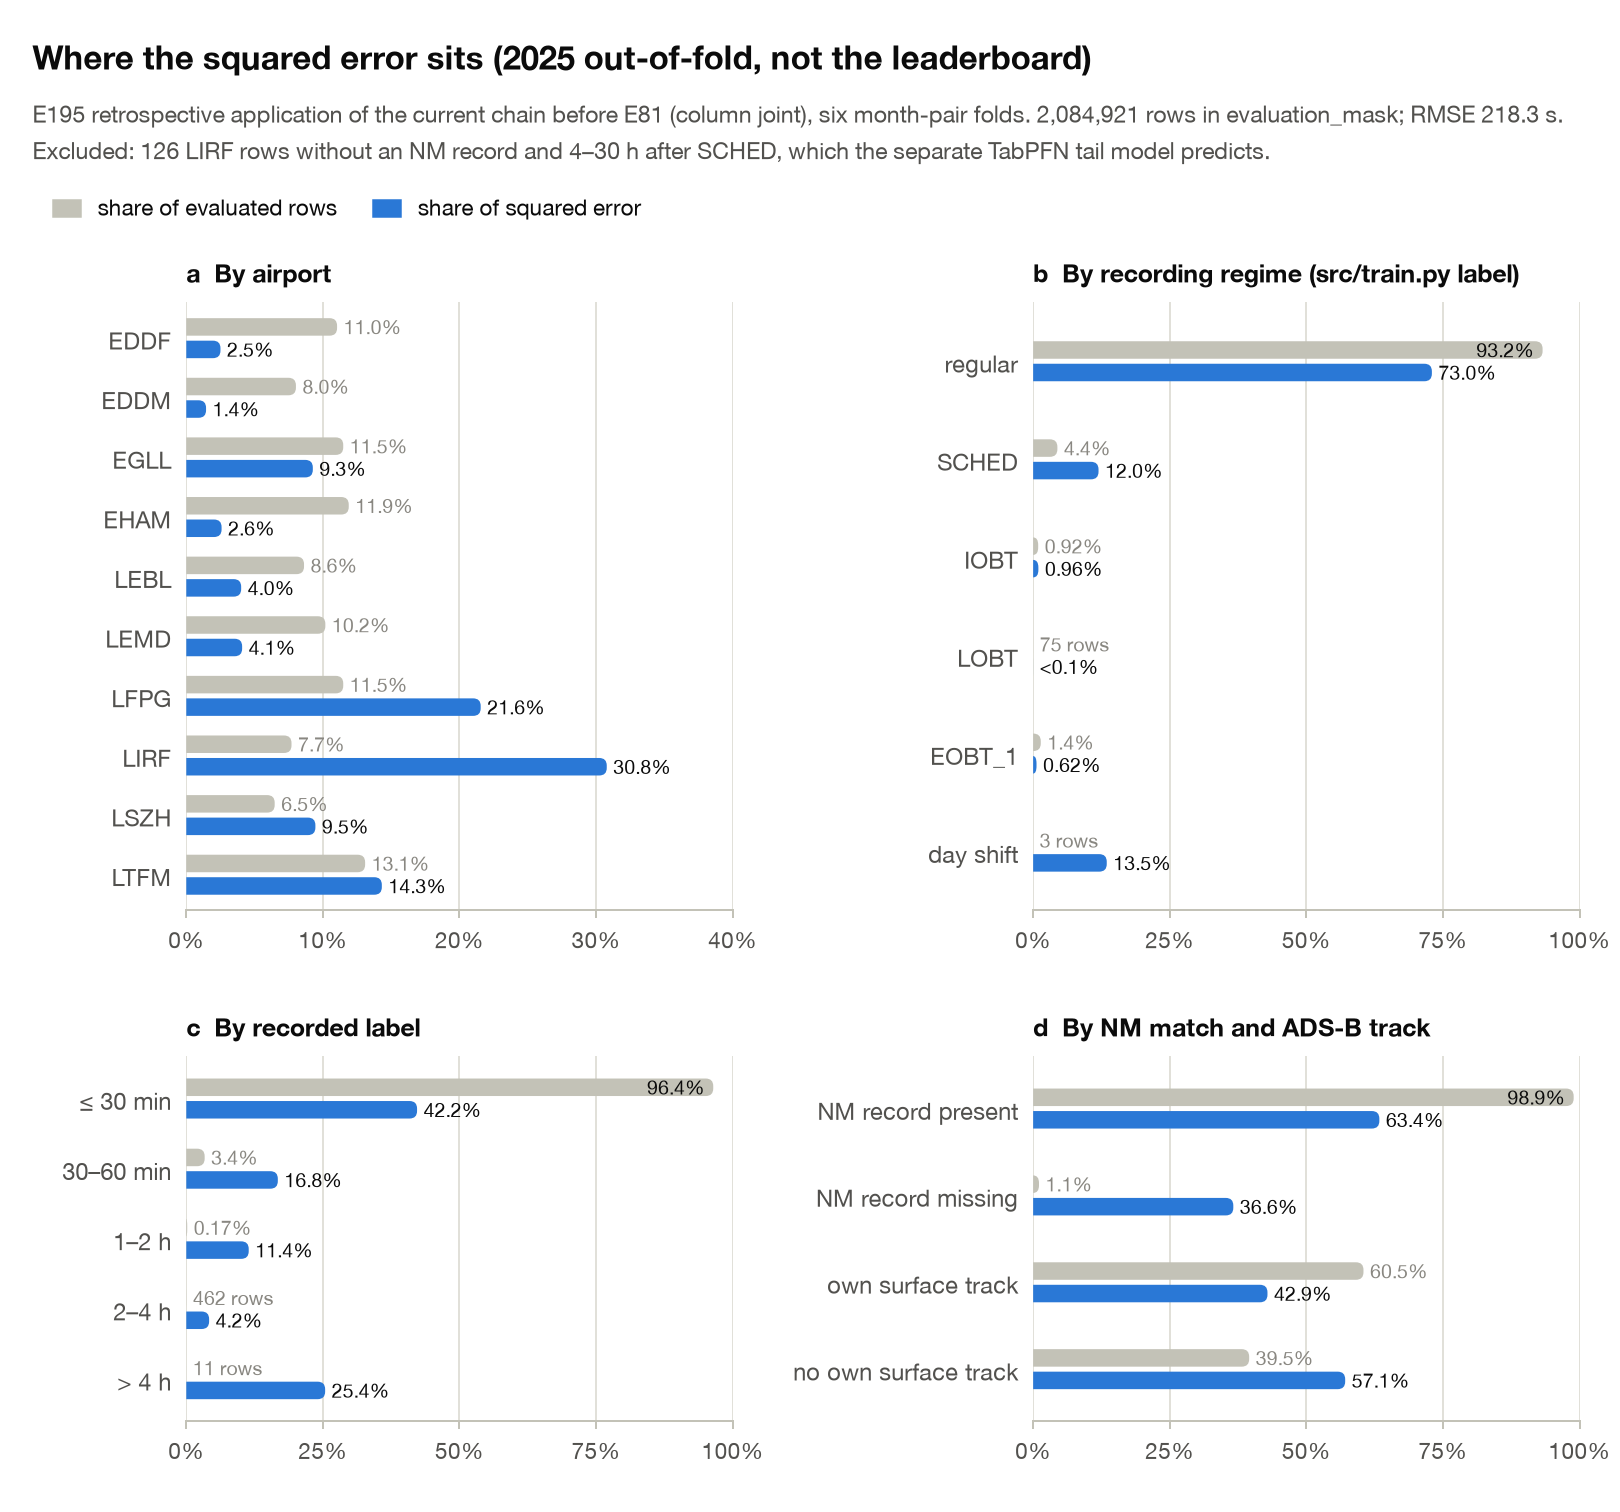
\includegraphics[width=\textwidth]{fig5_error_budget.png}}
\caption{Share of rows against share of squared error in 2025 out-of-fold predictions, by airport, recording regime, label size, NM match and ADS-B track.}\label{fig:4}
\end{figure}

The chain has a dedicated component wherever the error concentrates: the LIRF tail without NM has its own model, rows without LOBT outside LIRF get a movement-only member, and the ADS-B stages correct the start of taxi where a track exists. On labels up to 7,200 s the largest airport errors after LIRF (363.5 s) are LTFM (224.2 s) and LFPG (211.9 s): one has no surface tracks and the most biased proxy, the other has tracks for at most a quarter of its departures. These remain the open problems.

\section{Method}\label{method}

\subsection{Overview}\label{overview}

Figure~\ref{fig:5} shows the chain of the best ordinary submission, v12077, which is the v12075 chain of 7 October with two zero-fit changes made on 8 October: the neural member is the mean of ten seeds instead of three, and its weight in the regular candidate is 0.35 instead of 0.25 (Section 3.4). A feature table (FIN1b) feeds a regime classifier and a regular-duration candidate; the two combine into a probability-weighted mixture; surface stages correct the mixture where a track exists, subject to a gate; final controls blend with two earlier pipelines, enforce the LOBT window, protect 42 frozen tail predictions and apply a half-weight OPDI correction at LSZH. The final four-month file uses the same chain with the blend and the frozen rows removed (Section 3.8).

\begin{figure}[htbp]
\centering
{\scriptsize\begin{verbatim}
Challenge data (movements + NM timestamps) --+
METAR, OSM geometry, ATFM aggregates --------+--> Feature table FIN1b (170 tree / 189 neural columns)
                                             |        |                      |
                                             |        v                      v
                                             |  Regime classifier      Regular-duration candidate:
                                             |  LightGBM, 6 classes    CatBoost + LightGBM residual to NM proxy
                                             |                         + 5 anchored LightGBM members
adsb.lol surface tracks ---------------------+------------------------ + ordered-trajectory neural member (0.35, 10 seeds)
                                             |        |                      |
                                             |        +----------+-----------+
                                             |                   v
                                             |   Probability-weighted mixture (regular / SCHED / IOBT / LOBT / EOBT / +1 day)
                                             |                   v
                                             +--> Surface stages: own track (E141), previous visit (E64, E188)
                                                                 v
                                                  Gate: keep pre-surface value if a planning regime has p >= 0.95 (E152)
                                                                 v
                                                  Final controls: blend with v44/v60 (E81; absent in the final), LOBT window,
                                                  tail rows protected (42 frozen in v12077; all served rows in the final),
                                                  LSZH OPDI correction at 50 %
                                                                 v
                                                             Submission
\end{verbatim}}
\caption{Stage order of the submitted chain (v12077; the final file differs as marked). Experiment identifiers (E-numbers) are those of the repository's experiment register.}\label{fig:5}
\end{figure}

\subsection{Features}\label{features}

The final feature table FIN1b has 170 columns for the tree models and 189 for the neural member (Table~\ref{tab:1}). Most are built from the challenge data: the planning-time intervals (take-off minus each NM timestamp, \texttt{AOBT\_\allowbreak{}3} minus EOBT\_1, a flag for an \texttt{AOBT\_\allowbreak{}3} more than 3,606 s from the LOBT); airport, runway, aircraft and flight identity, including the airline prefix parsed from the flight number; traffic counts at the airport and on the runway around the flight; neighbour NM taxi proxies (other departures' take-off minus \texttt{AOBT\_\allowbreak{}3} by airport, runway and stand); neighbour features ordered by filed times (take-off minus LOBT and minus schedule of other departures); stand turnaround; forward neighbours (departures in the next 15--60 min); planned-arrival residuals; and runway wake-separation features. External features are METAR weather, stand-to-runway geometry and taxi-route length on the OpenStreetMap taxiway graph, and the destination airport's daily arrival ATFM delay.

{
\begin{longtable}[]{@{}
  >{\raggedright\arraybackslash}p{(\linewidth - 6\tabcolsep) * \real{0.2143}}
  >{\raggedright\arraybackslash}p{(\linewidth - 6\tabcolsep) * \real{0.2143}}
  >{\raggedleft\arraybackslash}p{(\linewidth - 6\tabcolsep) * \real{0.2857}}
  >{\raggedleft\arraybackslash}p{(\linewidth - 6\tabcolsep) * \real{0.2857}}@{}}
\caption{Feature families of FIN1b and their share of the total split gain in the saved regime classifier and LightGBM regressor.}\label{tab:1}\tabularnewline
\toprule\noalign{}
\begin{minipage}[b]{\linewidth}\raggedright
Family
\end{minipage} & \begin{minipage}[b]{\linewidth}\raggedright
Source
\end{minipage} & \begin{minipage}[b]{\linewidth}\raggedleft
Columns (trees / neural)
\end{minipage} & \begin{minipage}[b]{\linewidth}\raggedleft
Gain share: classifier / regressor
\end{minipage} \\
\midrule\noalign{}
\endfirsthead
\caption[]{(continued)}\tabularnewline
\toprule\noalign{}
\begin{minipage}[b]{\linewidth}\raggedright
Family
\end{minipage} & \begin{minipage}[b]{\linewidth}\raggedright
Source
\end{minipage} & \begin{minipage}[b]{\linewidth}\raggedleft
Columns (trees / neural)
\end{minipage} & \begin{minipage}[b]{\linewidth}\raggedleft
Gain share: classifier / regressor
\end{minipage} \\
\midrule\noalign{}
\endhead
\bottomrule\noalign{}
\endlastfoot
Planning-time intervals & Challenge data: movement and NM times & 11 / 11 & 40.4 \% / 36.7 \% \\
Airport, runway, aircraft, flight identity & Challenge data & 12 / 15 & 45.5 \% / 23.2 \% \\
Local time & Challenge data & 2 / 2 & 0.2 \% / 0.4 \% \\
Airport traffic counts & Challenge data: all movements & 28 / 28 & 1.2 \% / 3.3 \% \\
Runway traffic and configuration & Challenge data & 12 / 12 & 0.4 \% / 1.5 \% \\
Neighbour NM taxi proxies & Other departures' take-off $-$ \texttt{AOBT\_\allowbreak{}3} & 23 / 23 & 3.6 \% / 11.7 \% \\
Stand turnaround & Arrivals on the same stand & 4 / 4 & 1.0 \% / 3.4 \% \\
Forward neighbours & Departures in the next 15--60 min & 14 / 14 & 1.0 \% / 2.9 \% \\
Filed-time neighbours & Other departures' take-off $-$ LOBT or schedule & 27 / 27 & 3.9 \% / 8.7 \% \\
Planned-arrival residuals & NM planned arrival & 2 / 2 & 0.3 \% / 0.7 \% \\
Wake separation & Runway sequence and wake category & 7 / 7 & 0.5 \% / 1.2 \% \\
Weather (METAR) & Iowa Environmental Mesonet & 15 / 15 & 0.6 \% / 1.9 \% \\
Stand-to-runway geometry & OpenStreetMap & 5 / 5 & 0.6 \% / 1.8 \% \\
Taxi-route length & OpenStreetMap taxiway graph & 3 / 3 & 0.6 \% / 2.2 \% \\
Destination arrival ATFM delay & EUROCONTROL portal aggregates & 5 / 5 & 0.2 \% / 0.4 \% \\
Target encodings (month-out) & 2025 labels & 0 / 16 & --- \\
Ordered ADS-B observations & adsb.lol & 0 / 2 streams $\times$ 64 tokens $\times$ 12 channels & --- \\
\textbf{Total tabular columns} & & \textbf{170 / 189} & \textbf{100 \% / 100 \%} \\
\end{longtable}
}

All models drop the airport-day context, runway head- and crosswind, \texttt{month}, day of year and absolute timestamps. The tree models also drop stand identity, hourly runway configuration and all target encodings; each of these removals was tested on the leaderboard and improved it (Section 5.2). The neural member keeps these three groups; its target encodings exclude the row's own calendar month. Gain share measures training-loss reduction inside the boosters and is not the RMSE change from removing a feature; high-cardinality categoricals and correlated columns share credit.

\subsection{Recording-regime mixture}\label{recording-regime-mixture}

Let \(r(x)\) be the regular-duration prediction for a departure with features \(x\). The candidate vector contains \(r(x)\), the four take-off-minus-planning-time intervals (schedule, IOBT, LOBT, EOBT\_1) and \(r(x) + 86\,400\) for the one-day shift. A multiclass LightGBM \autocite{ke2017lightgbm} estimates regime probabilities \(p_k(x)\); infeasible or missing candidates are masked and the remaining probabilities renormalised. Before later corrections the prediction is

\begin{equation}\hat y(x) = \sum_k p_k(x)\, c_k(x),\end{equation}

the probability-weighted mean of the candidates. Under squared-error loss this is the optimal point prediction when the probabilities and the candidates' conditional means are correct. Section 5.5 shows that the same two arrays define a predictive distribution per flight whose central intervals are calibrated to within one point of nominal on 2025 out-of-fold rows, and Section 5.6 that the classifier's expected counts of planning copies agree with the labelled counts to within 0.1 percentage point per airport. The two-class version of this idea (schedule copy versus regular) removed 135.0 s of leaderboard RMSE on the first day; six classes, weather and geometry removed 27.0 s more (Section 5.1).

The classifier uses cost weighting when the feasible candidates span more than 3,600 s: the row weight is (spread / 3,600)\textsuperscript{2}, capped at 400; rows with smaller spread keep weight one. This emphasises regime errors that are expensive under RMSE and is an approximation to minimising the final mixture's error. Explicit LOBT-window rules (E167) rule out regimes that are impossible given the LOBT, for example a schedule-copy label more than an hour away from the LOBT.

Several alternatives were measured and rejected: a hard regime choice at a probability threshold (+29 s at $\tau$ = 0.5 in out-of-fold error), per-row choice among the four planning times, a neural classifier (better log-loss, worse mixture), training the classifier on mixture error, stacking the regressor's out-of-fold predictions into the classifier, adversarial-validation sample weights (+1.77 s on the leaderboard), and, on 8 October, an exact eleven-parameter recalibration of the regime probabilities fitted on 2025 out-of-fold rows and replayed through the frozen chain (E214): in-sample it removed 0.74 s, out of fold by month pair it added 0.41 s and forward in time 2.61 s, because the frozen surface stages and the gate were trained on the uncalibrated probabilities and any shift of \(p\) misaligns them. The repository's negative-results document lists these with effects.

\subsection{Regular-duration candidate}\label{regular-duration-candidate}

\textbf{Residual to a calibrated NM proxy.} The ordinary regressors do not learn the label directly. They learn the residual to an NM proxy: take-off minus \texttt{AOBT\_\allowbreak{}3} where it exists and lies within 0--7,200 s, else take-off minus LOBT, else minus EOBT\_1. The proxy is scaled by a least-squares coefficient per airport and timestamp source, shrunk towards a global value (E46); the fitted \texttt{AOBT\_\allowbreak{}3} scales are 0.80--1.16 and the LOBT scales 0.42--0.69. An airport median is the fallback when no proxy exists. The regressor's training target is clipped to 0--7,200 s; longer labels are left to the regime mixture and the tail model. Learning the residual to the proxy, together with neighbour features, gave $-$32.6 s on the leaderboard (v7 against v5).

A consequence that we measured and used throughout is that a residual model absorbs any input change it can express: on six folds a change in the \emph{level} of the proxy was absorbed by 95--99 \% and a change in its \emph{shape} by 65--68 \%. An isotonic calibration made the proxy more accurate (RMSE 378 $\rightarrow$ 346 s) and the final prediction worse (+0.46 s). A better intermediate quantity is not a better result.

\textbf{Members.} The regular candidate is a fixed-weight combination (Table~\ref{tab:2}). The core is 0.65 $\times$ CatBoost \autocite{prokhorenkova2018catboost} (15 seeds) + 0.35 $\times$ LightGBM (5 seeds), both on the proxy residual. Five further LightGBM members add diversity: one learns the raw target and four learn it relative to clipped take-off-minus-T anchors for T = LOBT, schedule, EOBT\_1 and \texttt{AOBT\_\allowbreak{}3}. Each uses a five-seed average. Their weights were fitted on 2025 out-of-fold predictions and then scaled to 2/3 after a comparison of complete files on the leaderboard (Section 6.3). For rows without a LOBT outside LIRF (4,907 ranking rows), a movement-only member built from ADS-B motion features replaces 7/30 of the regular candidate (E185).

{
\begin{longtable}[]{@{}
  >{\raggedright\arraybackslash}p{(\linewidth - 4\tabcolsep) * \real{0.2727}}
  >{\raggedleft\arraybackslash}p{(\linewidth - 4\tabcolsep) * \real{0.3636}}
  >{\raggedleft\arraybackslash}p{(\linewidth - 4\tabcolsep) * \real{0.3636}}@{}}
\caption{Fixed weights inside the regular-duration candidate: v12075 and v12077 (the final file uses the v12077 column).}\label{tab:2}\tabularnewline
\toprule\noalign{}
\begin{minipage}[b]{\linewidth}\raggedright
Component
\end{minipage} & \begin{minipage}[b]{\linewidth}\raggedleft
v12075
\end{minipage} & \begin{minipage}[b]{\linewidth}\raggedleft
v12077 and final
\end{minipage} \\
\midrule\noalign{}
\endfirsthead
\caption[]{(continued)}\tabularnewline
\toprule\noalign{}
\begin{minipage}[b]{\linewidth}\raggedright
Component
\end{minipage} & \begin{minipage}[b]{\linewidth}\raggedleft
v12075
\end{minipage} & \begin{minipage}[b]{\linewidth}\raggedleft
v12077 and final
\end{minipage} \\
\midrule\noalign{}
\endhead
\bottomrule\noalign{}
\endlastfoot
Residual blend 0.65 $\times$ CatBoost (15 seeds) + 0.35 $\times$ LightGBM (5 seeds) & 19/60 & 0.27444 (remainder) \\
Raw-target LightGBM member & 1/30 & 0.028889 \\
LOBT-anchored LightGBM member & 0.10 & 0.086667 \\
Schedule-anchored LightGBM member & 0.10 & 0.086667 \\
EOBT-anchored LightGBM member & 0.10 & 0.086667 \\
AOBT-anchored LightGBM member & 0.10 & 0.086667 \\
Ordered-trajectory neural member & 0.25, mean of 3 seeds & 0.35, mean of 10 seeds \\
\end{longtable}
}

\textbf{Neural member with ordered trajectories.} The last member is a multilayer perceptron with piecewise-linear numerical embeddings \autocite{gorishniy2022embeddings} (48-bin training quantiles, 12 embedding dimensions, width 512; \texttt{rtdl\_\allowbreak{}num\_\allowbreak{}embeddings} 0.0.12, version-B preset), trained for eight epochs with AdamW, learning rate 0.002, weight decay 10\textsuperscript{$-$5} and OneCycleLR. It reads 189 tabular columns and, in addition, up to 64 ordered ADS-B observations of the current visit and of the previous visit of the same aircraft to the airport: time to take-off, position, altitude, speed, heading and on-ground flag, twelve channels with missingness masks, processed by message blocks over previous, current and next tokens (E197/E203). It is not a graph of interacting flights. Each seed has 1,908,437 parameters and took about 269 s to fit on an AMD Radeon RX 7900 XTX. The member replaced an earlier tabular-only version (E190) at the same weight and gained 0.51 s on the leaderboard. Its component-level advantage over the previous member (4.5--7.1 s on two month-pair screens) was much larger than its full-chain effect; against an equal-capacity control without ordering it won only 0.25 and 0.13 s on the same pairs, so most of the component-level gain reflects changed inputs and capacity, not ordering alone. Twelve epochs instead of eight (E215) lowered the pooled 2025 error by 0.107 s but made February worse by 1.61 s in all three seeds, failed its gate and was not used.

\textbf{Seeds and weight (E212).} The weight 0.25 had been inherited from the earlier MLP member and had never been chosen at the level of the full chain. On 8 October the exact 2025 out-of-fold chain up to the blend was recomputed at twelve weights (0.05--0.60 in steps of 0.05) with the three-seed and a ten-seed member, the weight being taken from the other members in proportion; at \(w = 0.25\) this reproduces the production column byte for byte on all 2,085,047 rows. Pooled over the six month pairs on the decided rows the RMSE is 217.717 s at 0.25, 217.549 s at 0.35 and 217.523 s at 0.40 with three seeds, and 217.723, 217.535 and 217.496 s with ten seeds; the ten seeds alone at the old weight change nothing (+0.0065 s). The registered leave-one-pair-out rule selected 0.40 in all six pairs ($-$0.228 s pooled, gate passed). Two checks outside the gate argued for less: 0.40 is worse than 0.25 in August (+0.016 s), and a weight chosen on January--June (0.50) is worse than 0.25 on July--December (+0.017 s); the per-month optimum ranges from 0.30 to 0.60 (Table~\ref{tab:10} and Figure~\ref{fig:9} in Section 5.4). We fixed 0.35 instead, the only grid value with lower squared error than 0.25 in every month of 2025 at three and at ten seeds (Figure~\ref{fig:9}), and wrote it into the final assembler before any upload. The two changes were then scored on the leaderboard as single-change uploads with forecasts written beforehand: v12076 (ten-seed mean at 0.25) 230.8183 s, $-$0.1204 s against v12075, inside its corridor; v12077 (weight 0.35) 230.4812 s, $-$0.3371 s against v12076, 0.14 s better than the lower edge of a corridor derived from the January + July 2025 estimate of $-$0.11 s times a 0.7 transfer factor. The weight shift transferred to the board about three times stronger than its out-of-fold estimate.

\subsection{Surface stages from the aircraft's own track}\label{surface-stages-from-the-aircrafts-own-track}

Where the flight's own adsb.lol ground track exists, gradient-boosted stages correct the mixture output. The extraction, run day by day over the archive (about 3.5--4 GB per day, processed as a stream), yields the first ground fix, the first movement after the stand at a 1-knot threshold, the stops and their ends, the path length, distances of track points to the assigned stand, the time of leaving a 150 m zone around it, and a kinematic estimate of the unseen start of the taxi from the distance at the first fix and the initial speed. Lowering the movement threshold from 3 kt to 1 kt reduced the median error against known block times from 302.6 s to 193.5 s on 18,050 departures. The stored surface files also hold airborne points of the same aircraft within 7 km and below 2,500 ft; these supply \emph{previous-visit} features, the aircraft's earlier arrival at the airport.

Two populations are corrected by disjoint stages. The own-track stage (E141) corrects rows with an own surface track; the previous-visit stage (E64) corrects rows without one that have a previous visit. Both are small LightGBM models on the residual of the mixture, trained on all rows including those where the record contradicts the track, averaged over seeds 42, 1, 2, 3 and 4, with their target clipped to $\pm$1,800 s. Seven reception-density features are dropped from E141 and three from E64 because their behaviour did not transfer between 2025 and 2026. A third stage (E188) retrains the previous-visit correction for LIRF rows that have an NM record, no own track and a previous visit; its incremental evidence is small and mixed (Section 4.1), and on its own mask its sign varies by month (June +0.79 s, July +3.66 s, year $-$0.29 s in 2025); it stays because removing it would be a design change. A gate (E152) restores the pre-surface prediction when the maximum probability of the four planning-time classes is at least 0.95, because physical movement cannot explain a label that is a copy of a planning time. The gate is based on model confidence, not on knowledge of the true regime.

The stages are inert where no track exists, by mask and verified on out-of-fold data (0 rows changed outside the masks). In the final file E141 changed 429,789 of 670,790 rows, E64 95,421 and E188 18,128; in LIRF June 2026 58.8 \% of rows are touched by no ADS-B stage. The neural member sees empty trajectory tokens on such rows; an audit on 2025 out-of-fold data found that without tokens it behaves like a tabular network (RMSE 389.1 s against 388.9 s for the tabular member on 510,582 rows) and is still better than no neural member in every fold and in each collapsed airport-month, so a pre-registered protection rule (weight 0 without tokens) failed its gate (0 of 6 folds, +2.03 s on the rows it touched) and was not applied. A scenario estimate of the cost of the lost coverage on the final file is about +0.18 s (range +0.1 to +0.3 s); it transfers 2025 penalties to the 2026 masks and is not a measurement.

The first surface stage gave $-$15.2 s on the leaderboard; stand geometry $-$3.7 s; previous visits $-$2.5 s; the 1-knot threshold $-$0.6 s. We note that the technique of extracting ground tracks from adsb.lol had been seen in another team's public code; the implementation is ours. A replacement of the learned stages by a fixed physical estimate (take-off minus first movement, with a lag fitted on the other half-year) was measured and rejected: +20.5 s on the body subset and +18.3 s on decided rows, and even a perfect per-row selector between the learned and the physical estimate would have gained at most 0.69--0.86 s. Coverage bounds the stages: full ground coverage would be worth about 28 s on the ranking set, but LFPG, LIRF in July and LTFM are almost unobserved in any open archive.

\subsection{Sparse Rome tail}\label{sparse-rome-tail}

LIRF departures without an NM match and 4--30 h after schedule have few examples and very different possible values (minutes or hours; for rows 12--30 h late, 39 \% were shifted by one day). Their regime probabilities come from a TabPFN-2 classifier \autocite{hollmann2025tabpfn} with the airline prefix and the local date as features, replacing an empirical regime table ($-$27.0 s) and then improving on it ($-$4.7 s; a leave-one-month-out squared error $-$41.5 \%, better in 11 of 12 months). Adding the airline prefix to the tail model changed only 42 ranking rows and gained 3.60 s on the leaderboard, although it had failed a ``better in at least 8 of 12 months'' rule (6 of 12); the rule counted months with 4--6 rows like months with 39 and was withdrawn. A reviewer found that 65.1 \% of the tail table's holdout gain came from three rows. The tail is where the score is most fragile. Twenty seeds instead of ten, and averaging the ensemble over $\pm$6 s shifts of its input times, were tested leave-one-month-out on the 2025 tail on 8 October (E210): all variants failed the gate written before the run (squared error +0.005 \% to +0.13 \%, June worse in each), so the stage keeps ten seeds.

TabPFN inference is not bit-identical across runs and machines in general: 39 of the 42 rows differed between an x86 and an Apple-Silicon run. The ordinary submissions therefore copy these 42 predictions from a fixed earlier submission (v361, a single draw) and restore them after all later stages. This preserves the output across builds but makes the donor file an explicit dependency, and it is not a rule for choosing rows in a new period. The final file does not use the donor rows: a fresh ten-seed ensemble serves every row of the tail segment in all four months, and on the sealed input it was bitwise repeatable (two runs, identical probabilities for all ten seeds, 0 of 62 rounded values differing; Section 3.8).

\subsection{Final controls}\label{final-controls}

After the gate, the whole file is blended with two earlier complete pipelines that had lost as replacements but carried partly independent information: v44 (per-airport classifiers and regressors, 256.34 s on the leaderboard) and v60 (an earlier global chain with ADS-B features inside the base, 252.10 s). Their 2025 cross-validation residuals correlated with the accepted chain at 0.939 and 0.964. Under squared error a small weight on a partner lowers the error when $\rho$$\cdot$$\sigma$\_partner \textless{} $\sigma$\_main. The weights were fitted by non-negative least squares on 2025 out-of-fold predictions against the chain of 20 September and fixed since:

\begin{equation}p_{\mathrm{E81}} = 0.8516\,p_{\mathrm{current}} + 0.1214\,p_{\mathrm{v44}} + 0.0270\,p_{\mathrm{v60}}.\end{equation}

Complete out-of-fold counterparts of v44 and v60 were not kept, so both donors enter only as archived ranking files; this is the main obstacle to a fully nested validation (Section 4.1), and the donors exist only for January and July 2026, so the blend cannot be carried to a new period. Its price on the v12077 chain was measured on 9 October by one upload with the blend skipped: +0.5676 s (Section 5.7). An adjustment near the lower edge of the LOBT window and a clip to the feasibility window follow, then the 42 protected tail values are restored. The last stage fits a small LightGBM residual model on OPDI exit-parking and taxiway events at LSZH only (inputs: OPDI duration, its difference from the prediction, the prediction, the exit-to-taxiway interval) and blends the corrected and uncorrected files 50:50. The same correction at EDDF, which had no labels for calibration, worsened the leaderboard by 1.13 s and was dropped; at LSZH it gave $-$0.13 s against a leave-one-month-out forecast of $-$1.2 s.

\subsection{The uniform recipe for the blind final}\label{the-uniform-recipe-for-the-blind-final}

The final file \texttt{gentle-igloo\_\allowbreak{}final.parquet} is produced by one procedure over all 670,790 rows of the four months. It is the v12077 chain with the two leaderboard-specific parts removed (Table~\ref{tab:3}): the whole-file blend with the archived January/July submissions, and the 42 frozen tail rows. The tabular members were refitted with the same rounds, seeds and weights on the feature table rebuilt against the four-month file (2,755,837 rows = 2,085,047 training + 670,790 final; 52 fits, models saved this time); the ten-seed neural member was retrained on the same recipe with the 2026 days re-encoded on the final movement times; the surface-stage models, the gate, the LOBT window and the LSZH model are the cached 2025 models, replayed only when the reconstructed training call matches the stored signature. Nothing is chosen per month.

{
\begin{longtable}[]{@{}
  >{\raggedright\arraybackslash}p{(\linewidth - 4\tabcolsep) * \real{0.3333}}
  >{\raggedright\arraybackslash}p{(\linewidth - 4\tabcolsep) * \real{0.3333}}
  >{\raggedright\arraybackslash}p{(\linewidth - 4\tabcolsep) * \real{0.3333}}@{}}
\caption{The best ordinary file and the final file.}\label{tab:3}\tabularnewline
\toprule\noalign{}
\begin{minipage}[b]{\linewidth}\raggedright
\end{minipage} & \begin{minipage}[b]{\linewidth}\raggedright
v12077 (leaderboard)
\end{minipage} & \begin{minipage}[b]{\linewidth}\raggedright
\texttt{gentle-igloo\_\allowbreak{}final.parquet}
\end{minipage} \\
\midrule\noalign{}
\endfirsthead
\caption[]{(continued)}\tabularnewline
\toprule\noalign{}
\begin{minipage}[b]{\linewidth}\raggedright
\end{minipage} & \begin{minipage}[b]{\linewidth}\raggedright
v12077 (leaderboard)
\end{minipage} & \begin{minipage}[b]{\linewidth}\raggedright
\texttt{gentle-igloo\_\allowbreak{}final.parquet}
\end{minipage} \\
\midrule\noalign{}
\endhead
\bottomrule\noalign{}
\endlastfoot
Feature table & FIN1b on 2025 + January/July ranking file & FIN1b rebuilt on 2025 + four-month file \\
Base classifier, regressors, anchored and movement-only members & Fitted on the January/July view & Refitted with the same recipe on the four-month view (52 fits, saved) \\
Neural member & 0.35, ten seeds, fitted on the January/July view & 0.35, ten seeds, fitted on the four-month view \\
Whole-file blend with v44 and v60 (E81) & Present & Absent (nothing equivalent exists for February and June) \\
LIRF tail without an NM record & 42 rows frozen from one TabPFN draw & Fresh ten-seed TabPFN-2 ensemble on every row of the tail segment (62 served rows), protected from later stages \\
Surface stages, gate, LOBT window, LSZH stage at 50 \% & Present & Present, cached models replayed; OPDI events extracted for February and June so that the LSZH stage acts in all months (LSZH rows with an event: 41.5 / 73.5 / 76.8 / 77.0 \% by month) \\
Input timestamps & Old ranking file & Final ranking file with its $\pm$12 s shifts, as published \\
\end{longtable}
}

Two alternatives were rejected in writing before the assembly: copying the v12077 rows into the January/July part of the final and predicting only February and June with a model (two procedures in one file, exactly what the organiser named as the reason for the blind final), and keeping the January/July blend donors. The 0.35 weight and the ten-seed mean were decided on 2025 data before the two confirming uploads (Section 3.4). The assembly, validation, replay and the measured price of the recipe are reported in Section 5.7.

\section{Validation}\label{validation}

\subsection{Temporal month-pair cross-validation}\label{temporal-month-pair-cross-validation}

The main scheme has six outer folds of 2025: months 1+7, 2+8, 3+9, 4+10, 5+11 and 6+12. Each fold holds out both months and trains on the other ten, mirroring the January + July ranking set. Where boosting rounds are selected, the month after each held-out month serves as the inner validation month and the selected iteration count is used for a refit on the outer training months. Candidate and control are compared on identical rows by paired squared error. An integrity checker verifies fold inventory, unique IDs within and across folds, complete coverage of training IDs, targets against the feature table, held-out months, shapes and finite values; later evaluators also bind input hashes, seed receipts and stage outputs. These checks establish artifact consistency; they cannot establish that every upstream model was independently cross-fitted.

Three subsets are reported. \emph{Decided} excludes the LIRF rows without an NM record and 4 h or more after schedule, which a separate tail model serves (2,084,920 of 2,085,047 rows). \emph{Body} is rows with observed target $\le$ 7,200 s (2,084,448 rows). \emph{Trimmed} removes the three or twenty largest and smallest paired differences in each fold. Body is defined by the label and is a diagnostic, not a routing condition (Section 4.3).

A caveat applies to all cross-validation results of the final chain. Some later stages were trained on historical out-of-fold predictions of earlier ones, the stored classifier probabilities are already feasibility-masked, and exact out-of-fold donors for the E81 blend are unavailable. The retrospective comparison of the current members (E195, E203, E212) therefore runs through the gate but \textbf{before the E81 blend, the LOBT adjustments, the tail protection and the LSZH stage}, and is \emph{selection-informed} validation: the production manifest records \texttt{quality\_\allowbreak{}validated\_\allowbreak{}on\_\allowbreak{}full\_\allowbreak{}chain\ =\ false}. Table~\ref{tab:4} gives the comparison for the last accepted members.

{
\begin{longtable}[]{@{}
  >{\raggedright\arraybackslash}p{(\linewidth - 10\tabcolsep) * \real{0.1304}}
  >{\raggedleft\arraybackslash}p{(\linewidth - 10\tabcolsep) * \real{0.1739}}
  >{\raggedleft\arraybackslash}p{(\linewidth - 10\tabcolsep) * \real{0.1739}}
  >{\raggedleft\arraybackslash}p{(\linewidth - 10\tabcolsep) * \real{0.1739}}
  >{\raggedleft\arraybackslash}p{(\linewidth - 10\tabcolsep) * \real{0.1739}}
  >{\raggedleft\arraybackslash}p{(\linewidth - 10\tabcolsep) * \real{0.1739}}@{}}
\caption{Retrospective six-fold comparison of the chain before the E81 blend (2025 out-of-fold RMSE, seconds).}\label{tab:4}\tabularnewline
\toprule\noalign{}
\begin{minipage}[b]{\linewidth}\raggedright
Variant
\end{minipage} & \begin{minipage}[b]{\linewidth}\raggedleft
Decided RMSE
\end{minipage} & \begin{minipage}[b]{\linewidth}\raggedleft
Change
\end{minipage} & \begin{minipage}[b]{\linewidth}\raggedleft
Body RMSE
\end{minipage} & \begin{minipage}[b]{\linewidth}\raggedleft
Change
\end{minipage} & \begin{minipage}[b]{\linewidth}\raggedleft
Pairs improved
\end{minipage} \\
\midrule\noalign{}
\endfirsthead
\caption[]{(continued)}\tabularnewline
\toprule\noalign{}
\begin{minipage}[b]{\linewidth}\raggedright
Variant
\end{minipage} & \begin{minipage}[b]{\linewidth}\raggedleft
Decided RMSE
\end{minipage} & \begin{minipage}[b]{\linewidth}\raggedleft
Change
\end{minipage} & \begin{minipage}[b]{\linewidth}\raggedleft
Body RMSE
\end{minipage} & \begin{minipage}[b]{\linewidth}\raggedleft
Change
\end{minipage} & \begin{minipage}[b]{\linewidth}\raggedleft
Pairs improved
\end{minipage} \\
\midrule\noalign{}
\endhead
\bottomrule\noalign{}
\endlastfoot
Control (previous MLP member, no E188) & 218.610 & --- & 183.541 & --- & --- \\
E190 neural member (PLE) & 218.270 & $-$0.340 & 183.174 & $-$0.366 & 6/6 \\
E188 LIRF previous-visit stage & 218.603 & $-$0.007 & 183.536 & $-$0.005 & 3/6 \\
E190 + E188 (v12074) & 218.263 & $-$0.347 & 183.169 & $-$0.372 & 6/6 \\
E203 ordered-trajectory member at 0.25, 3 seeds (v12075) & 217.717 & $-$0.546 vs v12074 & 182.555 & $-$0.614 vs v12074 & 6/6 \\
E203 at 0.25, 10 seeds (v12076) & 217.723 & +0.0065 vs v12075 & --- & --- & 5/6 \\
E203 at 0.35, 10 seeds, anchors $\times$ 0.65/0.75 (v12077, final) & 217.535 & $-$0.182 vs v12075 & --- & --- & 6/6 \\
\end{longtable}
}

The 2025 out-of-fold RMSE of the chain before the blend is 217.5--218.3 s; its leaderboard RMSE is 230.5 s. The two numbers cover different rows and stages: the out-of-fold figure spans twelve months, excludes the 126 LIRF tail rows (which hold 111 of the 122 labels above four hours) and stops before the blend and the LSZH stage; on January and July 2025 alone the out-of-fold RMSE is 279.2 s, and four labels above four hours hold 38.2 \% of that squared error. Inputs also shift between years (ADS-B coverage; the share of departures without an NM record, 1.53 \% against 1.08 \%), and the chain was developed by selecting changes on the same 2025 data, so its out-of-fold error is optimistic. We have not measured how much of the gap each factor explains.

\subsection{Pre-registration and gates}\label{pre-registration-and-gates}

Before each experiment the decision rule was written down. Early rules were ``$-$0.30 s and at least 4 of 6 folds''; later rules were ``at least 4 of 6, trimmed \textless{} 0, body \textless{} 0'' or ``both screen pairs improve''; the October rules added forward-in-time legs (train on months 1--6, test on 7--12; expanding window) after two calibrations fitted on month pairs failed forward (Section 5.8). From 20 September most uploads also carried a leaderboard forecast range recorded before the upload. In the October experiments the protocol and code were committed before the first model fit. Verdicts were applied as written; a later change of mind is logged as a new entry and does not edit the old one. The register holds 448 numbered entries from 23 September to 9 October 2026 and the working brief holds the earlier experiments; the most informative rejections are summarised in English in the repository.

Some rules were themselves revised when they failed. The fixed $-$0.30 s threshold was not derived from data and was removed; a stage change worth $-$0.137 s (6 of 6 folds) was uploaded anyway and gave $-$0.04 s. The ``8 of 12 months'' tail rule rejected a change that then gained 3.60 s. If the decided and trimmed measures differ by more than a factor of two, the trimmed one decides, because on the 21 September chain the ten worst out-of-fold rows held 24.3 \% of the squared error and the worst single row was worth 7.47 s on the leaderboard scale, 25 times the gate. One decision departed from its registered rule in the conservative direction: the neural weight rule chose 0.40 and 0.35 was taken on the per-month evidence (Section 3.4); the departure was taken on 2025 months, not on the ranking months.

Forecast corridors were themselves tested. Of the four uploads of 8--9 October that priced the final recipe or checked the final file, three scored inside the corridor written before the upload and one, the control of the final file, scored 0.02 s below it on the favourable side (Section 5.7). Its corridor allowed $\pm$0.3 s for the refit of the members and the new input dithering; the label-free analysis afterwards put the noise of such a control at $\pm$0.43--0.55 s (1$\sigma$). A corridor for a file whose members were refitted must be about twice as wide as the one we wrote. The rule attached to the corridor still did its job: it stopped the final upload until the deviation was explained.

\subsection{Transfer from cross-validation to the leaderboard}\label{transfer-from-cross-validation-to-the-leaderboard}

Most uploads from 20 September on carried a written forecast, which lets us compare the cross-validation effect of a single change with its leaderboard effect (Table~\ref{tab:5}). On 4 October this was calibrated on 38 single-change pairs, 15 of them recomputed from out-of-fold files. The leaderboard change followed the decided-row cross-validation change (Pearson 0.89, slope 1.06) and its body part (0.90), but not the y \textgreater{} 7,200 s tail (0.09); the sign agreed in only 60--70 \% of pairs.

{
\begin{longtable}[]{@{}
  >{\raggedright\arraybackslash}p{(\linewidth - 6\tabcolsep) * \real{0.2143}}
  >{\raggedright\arraybackslash}p{(\linewidth - 6\tabcolsep) * \real{0.2143}}
  >{\raggedleft\arraybackslash}p{(\linewidth - 6\tabcolsep) * \real{0.2857}}
  >{\raggedleft\arraybackslash}p{(\linewidth - 6\tabcolsep) * \real{0.2857}}@{}}
\caption{Cross-validation against leaderboard effect of single changes (seconds; negative is better). CV values before October are on a leaderboard-equivalent scale, comparable in sign and rough size.}\label{tab:5}\tabularnewline
\toprule\noalign{}
\begin{minipage}[b]{\linewidth}\raggedright
Change (leaderboard pair)
\end{minipage} & \begin{minipage}[b]{\linewidth}\raggedright
Kind
\end{minipage} & \begin{minipage}[b]{\linewidth}\raggedleft
CV
\end{minipage} & \begin{minipage}[b]{\linewidth}\raggedleft
Leaderboard
\end{minipage} \\
\midrule\noalign{}
\endfirsthead
\caption[]{(continued)}\tabularnewline
\toprule\noalign{}
\begin{minipage}[b]{\linewidth}\raggedright
Change (leaderboard pair)
\end{minipage} & \begin{minipage}[b]{\linewidth}\raggedright
Kind
\end{minipage} & \begin{minipage}[b]{\linewidth}\raggedleft
CV
\end{minipage} & \begin{minipage}[b]{\linewidth}\raggedleft
Leaderboard
\end{minipage} \\
\midrule\noalign{}
\endhead
\bottomrule\noalign{}
\endlastfoot
ADS-B own-track stage E25 (v27 vs v22) & observation of the flight & $-$9.53 & $-$15.22 \\
Stand geometry in the stage E36 (v30 vs v29) & observation of the flight & $-$2.98 & $-$3.71 \\
Previous visits E64+E65 (v78 vs v55) & observation of the flight & $-$2.37 & $-$2.65 \\
Filed-time neighbours E77 (v97 vs v82) & observation of other flights & $-$2.73 & $-$3.26 \\
Proxy scale E46 (v55 vs v30) & calibration, no new capacity & $-$0.40 & $-$1.00 \\
Airline prefix E106 (v195 vs v155) & recording rule & $-$0.58 & $-$1.28 \\
Classifier cost weights E89 (v115 vs v97) & loss weighting & $-$1.02 (body +11.27) & $-$1.18 \\
Ordered trajectories E203 (v12075 vs v12074) & neural member & $-$0.55 (before E81) & $-$0.51 \\
Ten seeds instead of three (v12076 vs v12075) & seed averaging, no new capacity & +0.0065 (decided, before E81) & $-$0.12 \\
Neural weight 0.25 $\rightarrow$ 0.35, E212 (v12077 vs v12076) & mixture weight, no new capacity & $-$0.19 (decided, pooled); about $-$0.11 on Jan + Jul 2025 & $-$0.34 \\
\texttt{month} removed E24 (v22 vs v18) & capacity removed & $-$2.18 & $-$0.87 \\
Target encodings removed E99 (v155 vs v115) & capacity removed & +0.94, 0 of 6 & $-$0.17 \\
Per-airport models E38 (v43 vs v30) & learned capacity & $-$10.98 & +3.79 \\
Regime shares by group E50 (v65 vs v30) & 2025 aggregates & $-$2.79 & +5.78 \\
Flight-number habit at LIRF with NM E133 (v249 vs v247) & 2025 aggregates & $-$0.72 & +0.36 \\
Anchored members E171--E173 (v808 vs v655) & members at 2/3 weight & about $-$1.24 & $-$0.98 \\
Destination ATFM delay E163 (v778 vs v655) & external aggregate & $-$0.76 & $-$0.17 \\
Monthly PRU calibration E145 (v448 vs v447) & calibration to external data & better in 6 of 6 & +0.11 \\
Airline prefix in TabPFN tail E118 (v316 vs v247) & 42 tail rows & forecast $-$0.27 & $-$3.60 \\
\end{longtable}
}

The ratio of leaderboard to decided-row cross-validation change by type of change was about 1.0 for ADS-B stages, about 0.7 for blend members, 0.2--0.3 for new base features, and zero or negative for rules and calibrations fitted on 2025 (the proxy scale was an exception); tail models and capacity removals were not scaled by cross-validation at all. Later forecasts used the cross-validation change times the type ratio. The last two rows of Table~\ref{tab:5} add one observation: a change of mixture weights with no new capacity transferred at about three times its out-of-fold estimate, and seed averaging that was neutral out of fold gained 0.12 s on the board; the forecast corridor for the weight change was missed on the favourable side. Five rules were derived from these observations.

\begin{enumerate}
\def\labelenumi{\arabic{enumi}.}
\tightlist
\item
  \emph{Observation transfers; training-period aggregates do not.} Changes that read what the flight did (ADS-B stages) or what other flights filed (filed-time neighbours) transferred at full size or more. Learned capacity on 2025 aggregates won in cross-validation and lost on the leaderboard (per-airport models, regime shares by group, ADS-B features inside the base model: CV $-$1.41, leaderboard +0.33).
\item
  \emph{Capacity-free changes transfer even through a failed gate.} The cost-weighted classifier failed the body leg because that subset is selected by the true label: any shift of probability towards long regimes looks worse there by construction. It gained 1.18 s on the leaderboard.
\item
  \emph{Removing 2025 capacity can transfer against cross-validation.} Removing target encodings was worse in all six folds and better on the leaderboard; cross-validation on 2025 cannot see the 2025$\rightarrow$2026 shift, so for removals it served only as a cost filter. This is not universal: four other removals made the leaderboard worse (+0.40 to +1.45 s).
\item
  \emph{Measure only rows the base model decides.} Later stages overwrite 10--45 LIRF tail rows per fold, which carried up to 62 \% of a fold's squared error; with them excluded, the per-airport models' cross-validation gain fell from $-$10.55 to $-$1.82 s.
\item
  \emph{Probes for group effects must be split by month, and calibrations must be tested forward in time.} A runway $\times$ configuration interaction showed a split-half correlation of +0.763 under a random split and $-$0.041 under a month split, because rows from the same hour fell into both random halves. A residual-level correction fitted on month pairs (E211) passed the pair gate ($-$0.102 s, 5 of 6) and lost on every forward leg (+0.08 to +0.16 s), because the final applies 2025 coefficients to later months, which is the forward case.
\end{enumerate}

Component-level gains also shrank in the full chain: a mixture-density head improved the body RMSE by 0.40 s as a component and worsened the decided RMSE by 0.05 s inside the chain; the wake-separation features went from $-$1.47 s on one fold to $-$0.13 s over six and $-$0.06 s after the chain changed. The control must be the production model's out-of-fold predictions: one change looked like $-$1.33 s against an older control and was +4.76 s against production predictions.

\subsection{Predicting blends of scored files without labels}\label{predicting-blends-of-scored-files-without-labels}

Every leaderboard score is an unweighted RMSE over the same 344,841 rows. For two scored files with predictions \(P_1\), \(P_2\), scores \(s_1\), \(s_2\) and root-mean-square difference \(d = \sqrt{\mathrm{mean}((P_1 - P_2)^2)}\), the errors \(e_i = P_i - y\) satisfy \(\mathrm{mean}(e_1 e_2) = (s_1^2 + s_2^2 - d^2)/2\), so the blend \(wP_1 + (1-w)P_2\) scores

\begin{equation}\mathrm{RMSE}^2 = w\,s_1^2 + (1-w)\,s_2^2 - w(1-w)\,d^2 .\end{equation}

No labels are needed. Seven blends were priced before upload and scored within 0.0009 s of the forecast (the residual is the rounding of the uploaded file to whole seconds). The identity served three purposes: to price a blend before spending a slot; to refuse a blend whose cross-validation weights promised $-$9.68 s but which the identity priced 5.20 s worse than the base file; and to expose a hidden component, when a blend with an unscored partner missed its forecast by 0.66 s and the identity gave the partner's own leaderboard RMSE as 338.46 s although it had trailed the control by only 7 \% in cross-validation. The rule that followed is to blend only complete, scored submissions. Leaderboard-optimal blend weights ($-$1.004 s instead of the $-$0.83 s achieved for the first blend) were computed and not used, because fitting weights to the leaderboard is probing.

The identity has a limit, learned on 9 October. It is exact for the unrounded blend of fixed files, so ``de-blending'' v12077 gives the score of the chain before the E81 blend as 230.54 s; but the file without the blend, v12078, differs from that de-blended file by the stages applied after the blend (the LOBT edge lift, the tail protection and the half-weight LSZH stage; RMS 5.48 s on 62,163 rows) and scored 231.05 s, 0.45 s worse than the identity's point. The difference is correlated with the residual (2$\cdot$cov = 204.9 s\textsuperscript{2} against RMS\textsuperscript{2} = 30.0 s\textsuperscript{2}), not noise. The identity cannot be carried across stages that act after the blend; the historical price of the blend was the better guide. Used within its limit, the identity also gives the exact score of a file that was never uploaded: v12079 differs from v12077 on exactly 42 rows, on which v12077 and v12078 agree, so v12078 with those 42 rows replaced scores \(\sqrt{231.0488^2 + 231.1770^2 - 230.4812^2} = 231.7429\) s. This file is the reference point for the control of Section 5.7.

\section{Results}\label{results}

\subsection{Leaderboard progression}\label{leaderboard-progression}

111 uploads between 13 September and 8 October 2026 produced 63 new best scores (Figure~\ref{fig:6}); three more on 9 October measured the final recipe and are reported in Section 5.7, for 114 in total. The 31 steps with a gain of about 0.3 s or more account for 267.9 s of the total 270.7 s improvement. Table~\ref{tab:6} groups them into seven phases; each gain is against the previous best file, and where an upload bundled changes the repository's development history gives the single-change control.

\begin{figure}
\centering
\pandocbounded{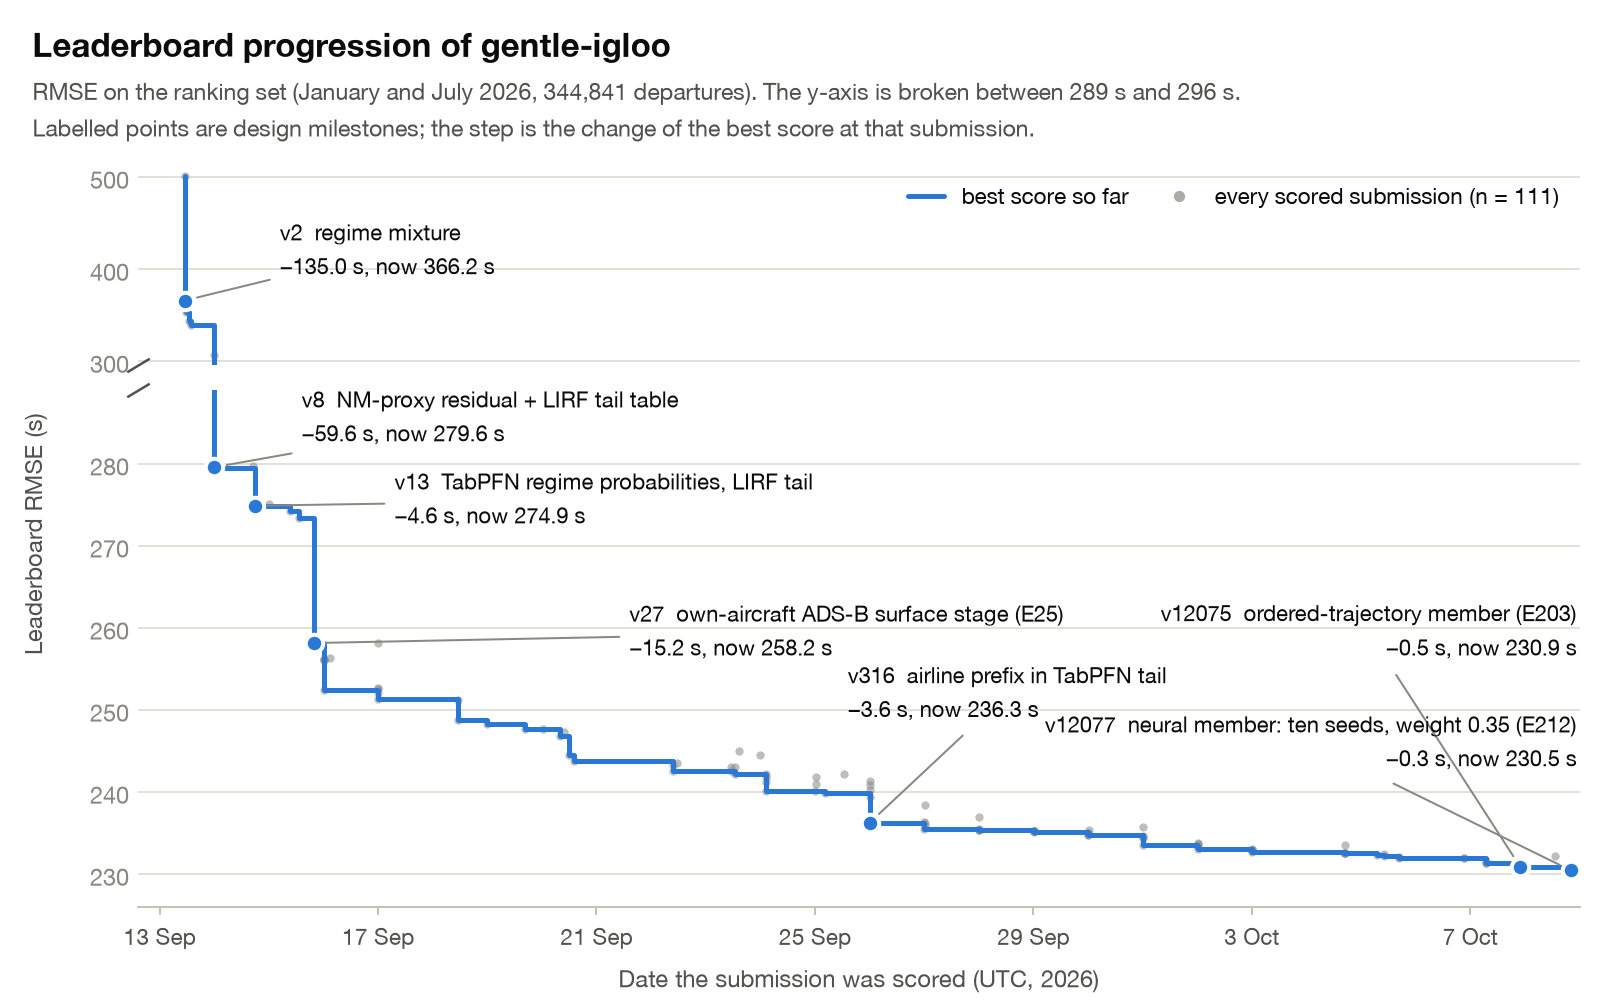
\includegraphics[width=\textwidth]{fig1_leaderboard_progression.png}}
\caption{Best leaderboard RMSE over time, from 501.23 s (v1, 13 September) to 230.48 s (v12077, 8 October), with labelled milestones.}\label{fig:6}
\end{figure}

{
\begin{longtable}[]{@{}
  >{\raggedright\arraybackslash}p{(\linewidth - 6\tabcolsep) * \real{0.2500}}
  >{\raggedright\arraybackslash}p{(\linewidth - 6\tabcolsep) * \real{0.2500}}
  >{\raggedright\arraybackslash}p{(\linewidth - 6\tabcolsep) * \real{0.2500}}
  >{\raggedright\arraybackslash}p{(\linewidth - 6\tabcolsep) * \real{0.2500}}@{}}
\caption{Phases of development and the design changes that moved the leaderboard score.}\label{tab:6}\tabularnewline
\toprule\noalign{}
\begin{minipage}[b]{\linewidth}\raggedright
Phase
\end{minipage} & \begin{minipage}[b]{\linewidth}\raggedright
Dates
\end{minipage} & \begin{minipage}[b]{\linewidth}\raggedright
Best RMSE (s)
\end{minipage} & \begin{minipage}[b]{\linewidth}\raggedright
Changes that moved the score (leaderboard gain, s)
\end{minipage} \\
\midrule\noalign{}
\endfirsthead
\caption[]{(continued)}\tabularnewline
\toprule\noalign{}
\begin{minipage}[b]{\linewidth}\raggedright
Phase
\end{minipage} & \begin{minipage}[b]{\linewidth}\raggedright
Dates
\end{minipage} & \begin{minipage}[b]{\linewidth}\raggedright
Best RMSE (s)
\end{minipage} & \begin{minipage}[b]{\linewidth}\raggedright
Changes that moved the score (leaderboard gain, s)
\end{minipage} \\
\midrule\noalign{}
\endhead
\bottomrule\noalign{}
\endlastfoot
1. Recording-regime mixture & 13 Sep & 501.2 $\rightarrow$ 339.2 & Two-regime mixture ($-$135.0); six regimes and METAR ($-$12.0); OSM geometry, hourly runway configuration, target encoding ($-$10.1); CatBoost + LightGBM ($-$4.8) \\
2. NM residuals and the Rome tail & 14--15 Sep & 339.2 $\rightarrow$ 273.4 & Residual to the NM proxy with neighbour features ($-$32.6); regime table for LIRF without NM ($-$27.0), then TabPFN-2 ($-$4.7); \texttt{month} removed ($-$0.9) \\
3. Own-aircraft ADS-B stages & 15--19 Sep & 273.4 $\rightarrow$ 247.8 & First surface stage ($-$15.2); extended features ($-$2.0); stand geometry ($-$3.7); per-airport proxy scale ($-$1.0); previous visit ($-$2.5); 1-knot threshold ($-$0.6) \\
4. Filed-time neighbours and blends & 20--23 Sep & 247.8 $\rightarrow$ 242.3 & Filed-time neighbours ($-$2.4); blends with v44 and v60 ($-$0.8, $-$0.7); cost-weighted classifier ($-$0.5) \\
5. Removing 2025-specific capacity & 24--27 Sep & 242.3 $\rightarrow$ 235.5 & Airline prefix for rows without NM ($-$0.4); stand identity and residual encodings removed ($-$0.7); airline prefix in the TabPFN tail ($-$3.6); CatBoost seed averaging ($-$0.8) \\
6. Stage refinements and members & 28 Sep -- 4 Oct & 235.5 $\rightarrow$ 232.6 & Anchored members ($-$1.0); MLP member ($-$0.4); planning-regime gate ($-$0.2); final feature table; several steps of 0.01--0.2 \\
7. Neural members with trajectories & 5--8 Oct & 232.6 $\rightarrow$ 230.5 & Movement-only member ($-$0.26); LSZH OPDI correction at half weight ($-$0.25 in two steps); piecewise-linear embeddings ($-$0.54); ordered ADS-B observations ($-$0.51); neural member as a mean of ten seeds ($-$0.12) and its weight raised from 0.25 to 0.35 ($-$0.34) \\
\end{longtable}
}

The largest gains came from describing the recording process ($-$135.0 s, then $-$27.0 s for the Rome tail) and from a physical sensor ($-$15.2 s for the first surface stage), not from learner tuning. After 26 September progress slowed: from 236.32 s to 230.48 s over 57 uploads. On 26 September the team was 8th of 192 and 3.14 s behind third place; on the morning of 8 October it was 14th of 237 and 15.32 s behind third place (215.62 s); at 20:15 UTC the same day, after v12077, it was 16th of 239 with third place at 213.5212 s, 16.96 s ahead, and on 9 October at 08:55 UTC third place stood at 213.2898 s. Leading teams improved much more in the same period. \placeholder{ final ranking --- rank of v12077 on the ordinary board at its close on 14 October 2026.}

\subsection{Single-change controls (ablations)}\label{single-change-controls-ablations}

Because each upload was a complete file scored on the same rows, the leaderboard provides single-change controls that are not available from cross-validation alone. Table~\ref{tab:7} collects the ones that define the submitted chain and the two measurement uploads of 9 October that price the parts removed for the final.

{
\begin{longtable}[]{@{}
  >{\raggedright\arraybackslash}p{(\linewidth - 4\tabcolsep) * \real{0.3000}}
  >{\raggedright\arraybackslash}p{(\linewidth - 4\tabcolsep) * \real{0.3000}}
  >{\raggedleft\arraybackslash}p{(\linewidth - 4\tabcolsep) * \real{0.4000}}@{}}
\caption{Single-change leaderboard controls (RMSE change in seconds; negative is better).}\label{tab:7}\tabularnewline
\toprule\noalign{}
\begin{minipage}[b]{\linewidth}\raggedright
Component
\end{minipage} & \begin{minipage}[b]{\linewidth}\raggedright
Control pair
\end{minipage} & \begin{minipage}[b]{\linewidth}\raggedleft
Effect
\end{minipage} \\
\midrule\noalign{}
\endfirsthead
\caption[]{(continued)}\tabularnewline
\toprule\noalign{}
\begin{minipage}[b]{\linewidth}\raggedright
Component
\end{minipage} & \begin{minipage}[b]{\linewidth}\raggedright
Control pair
\end{minipage} & \begin{minipage}[b]{\linewidth}\raggedleft
Effect
\end{minipage} \\
\midrule\noalign{}
\endhead
\bottomrule\noalign{}
\endlastfoot
Two-regime mixture instead of one regressor & v2 vs v1 & $-$135.01 \\
Residual to NM proxy + neighbour features & v7 vs v5 & $-$32.6 \\
Empirical regime table for LIRF without NM (42 rows) & v8 vs v7 & $-$27.0 \\
TabPFN-2 instead of the table (same rows) & v13 vs v8 & $-$4.70 \\
First ADS-B surface stage & v27 vs v22 & $-$15.22 \\
Stand geometry in the stage & v30 vs v29 & $-$3.71 \\
Per-airport $\times$ source proxy scale & v55 vs v30 & $-$1.00 \\
Previous-visit features & v78 vs v55 & $-$2.65 \\
1-kt movement threshold & v82 vs v80 & $-$0.58 \\
Filed-time neighbour features & v97 vs v82 & $-$3.26 \\
Cost-weighted regime classifier & v115 vs v97 & $-$1.18 \\
2025 target encodings removed from the regressor & v155 vs v115 & $-$0.17 \\
Airline prefix for rows without NM & v195 vs v155 & $-$1.28 \\
Stand identity + residual encodings removed & v225 vs v215 & $-$1.06 \\
Runway-configuration features removed & v245 vs v225 & $-$0.20 \\
Airline prefix in the TabPFN tail (42 rows) & v316 vs v247 & $-$3.60 \\
CatBoost five seeds & v285 vs v265 & $-$0.51 \\
Anchored members at 2/3 weight & v808 vs v655 & $-$0.98 \\
MLP member at 0.25 & v899 vs v859 & $-$0.78 \\
E81 blend and LOBT edge lift (dropping both) & v314 vs v316 & +0.69 \\
Movement-only member for rows without LOBT & v12008 vs v1139 & $-$0.26 \\
LSZH OPDI correction, full weight & v12060 vs v12048 & $-$0.14 \\
Piecewise-linear embeddings replacing the MLP & v12070 vs v12061 & $-$0.54 \\
Ordered-trajectory member replacing E190 & v12075 vs v12074 & $-$0.51 \\
Neural member: ten seeds instead of three & v12076 vs v12075 & $-$0.12 \\
Neural weight 0.35 instead of 0.25, anchors $\times$ 0.65/0.75 & v12077 vs v12076 & $-$0.34 \\
E81 whole-file blend removed (price of the blend on the v12077 chain) & v12078 vs v12077 & +0.57 \\
Fresh ten-seed TabPFN rows instead of the 42 frozen rows (price of the fresh tail) & v12079 vs v12077 & +0.70 \\
\end{longtable}
}

Changes that were tested the same way and made the leaderboard worse are part of the record: per-airport models (+3.79), regime shares by group (+5.78), ADS-B features inside the base model (+0.33), adversarial-validation weights (+1.77), the OPDI correction at EDDF (+1.13), a seed ensemble of the TabPFN tail (+0.86), monthly calibration to published PRU taxi-out times (+0.11), removal of the \texttt{ap\_\allowbreak{}runway} feature (+0.43) or of stand identity while keeping the encodings (+1.45).

\subsection{Out-of-fold error by airport}\label{out-of-fold-error-by-airport}

Table~\ref{tab:8} gives the 2025 out-of-fold RMSE by airport for the chain before the E81 blend (E195 \texttt{joint} arm, 2,084,921 rows; the 126 LIRF tail rows are excluded; the E203 member is not in these numbers). LIRF, LFPG and LTFM have the largest errors on labels up to 7,200 s. At LSZH six labels above 7,200 s hold 85 \% of the airport's squared error, which explains the gap between its two columns.

{
\begin{longtable}[]{@{}
  >{\raggedright\arraybackslash}p{(\linewidth - 8\tabcolsep) * \real{0.1579}}
  >{\raggedleft\arraybackslash}p{(\linewidth - 8\tabcolsep) * \real{0.2105}}
  >{\raggedleft\arraybackslash}p{(\linewidth - 8\tabcolsep) * \real{0.2105}}
  >{\raggedleft\arraybackslash}p{(\linewidth - 8\tabcolsep) * \real{0.2105}}
  >{\raggedleft\arraybackslash}p{(\linewidth - 8\tabcolsep) * \real{0.2105}}@{}}
\caption{2025 out-of-fold RMSE by airport, chain before the E81 blend.}\label{tab:8}\tabularnewline
\toprule\noalign{}
\begin{minipage}[b]{\linewidth}\raggedright
Airport
\end{minipage} & \begin{minipage}[b]{\linewidth}\raggedleft
Evaluated rows
\end{minipage} & \begin{minipage}[b]{\linewidth}\raggedleft
Share of squared error
\end{minipage} & \begin{minipage}[b]{\linewidth}\raggedleft
RMSE, all rows (s)
\end{minipage} & \begin{minipage}[b]{\linewidth}\raggedleft
RMSE, labels $\le$ 7,200 s (s)
\end{minipage} \\
\midrule\noalign{}
\endfirsthead
\caption[]{(continued)}\tabularnewline
\toprule\noalign{}
\begin{minipage}[b]{\linewidth}\raggedright
Airport
\end{minipage} & \begin{minipage}[b]{\linewidth}\raggedleft
Evaluated rows
\end{minipage} & \begin{minipage}[b]{\linewidth}\raggedleft
Share of squared error
\end{minipage} & \begin{minipage}[b]{\linewidth}\raggedleft
RMSE, all rows (s)
\end{minipage} & \begin{minipage}[b]{\linewidth}\raggedleft
RMSE, labels $\le$ 7,200 s (s)
\end{minipage} \\
\midrule\noalign{}
\endhead
\bottomrule\noalign{}
\endlastfoot
EDDF & 230,141 & 2.5 \% & 103.9 & 103.9 \\
EDDM & 167,334 & 1.4 \% & 92.7 & 92.7 \\
EGLL & 239,546 & 9.3 \% & 196.0 & 188.6 \\
EHAM & 247,951 & 2.6 \% & 101.7 & 98.5 \\
LEBL & 179,705 & 4.0 \% & 149.0 & 149.0 \\
LEMD & 212,242 & 4.1 \% & 138.3 & 138.3 \\
LFPG & 239,552 & 21.6 \% & 298.9 & 211.9 \\
LIRF & 160,578 & 30.8 \% & 436.4 & 363.5 \\
LSZH & 134,907 & 9.5 \% & 263.8 & 102.1 \\
LTFM & 272,965 & 14.3 \% & 228.2 & 224.2 \\
\textbf{All} & \textbf{2,084,921} & \textbf{100 \%} & \textbf{218.26} & \textbf{183.17} \\
\end{longtable}
}

\subsection{Generalisation across months: February and June as a pseudo-final}\label{generalisation-across-months-february-and-june-as-a-pseudo-final}

The blind final adds February and June, two months on which no file was ever scored. The six folds predict every 2025 month out of fold, so February and June 2025 serve as a pseudo-final for the same chain (Table~\ref{tab:9}; Figure~\ref{fig:7}). Confidence intervals are 95 \% percentile bootstraps that resample calendar days with replacement inside each group, so one day's flights move together.

{
\begin{longtable}[]{@{}
  >{\raggedright\arraybackslash}p{(\linewidth - 14\tabcolsep) * \real{0.1034}}
  >{\raggedleft\arraybackslash}p{(\linewidth - 14\tabcolsep) * \real{0.1379}}
  >{\raggedleft\arraybackslash}p{(\linewidth - 14\tabcolsep) * \real{0.1379}}
  >{\raggedright\arraybackslash}p{(\linewidth - 14\tabcolsep) * \real{0.1034}}
  >{\raggedleft\arraybackslash}p{(\linewidth - 14\tabcolsep) * \real{0.1379}}
  >{\raggedright\arraybackslash}p{(\linewidth - 14\tabcolsep) * \real{0.1034}}
  >{\raggedleft\arraybackslash}p{(\linewidth - 14\tabcolsep) * \real{0.1379}}
  >{\raggedleft\arraybackslash}p{(\linewidth - 14\tabcolsep) * \real{0.1379}}@{}}
\caption{2025 out-of-fold RMSE by month group, chain before the E81 blend (2,084,921 rows).}\label{tab:9}\tabularnewline
\toprule\noalign{}
\begin{minipage}[b]{\linewidth}\raggedright
Group
\end{minipage} & \begin{minipage}[b]{\linewidth}\raggedleft
Rows
\end{minipage} & \begin{minipage}[b]{\linewidth}\raggedleft
RMSE, all rows (s)
\end{minipage} & \begin{minipage}[b]{\linewidth}\raggedright
95 \% CI
\end{minipage} & \begin{minipage}[b]{\linewidth}\raggedleft
RMSE, body (s)
\end{minipage} & \begin{minipage}[b]{\linewidth}\raggedright
95 \% CI
\end{minipage} & \begin{minipage}[b]{\linewidth}\raggedleft
Labels \textgreater{} 4 h
\end{minipage} & \begin{minipage}[b]{\linewidth}\raggedleft
SSE in the 10 largest rows
\end{minipage} \\
\midrule\noalign{}
\endfirsthead
\caption[]{(continued)}\tabularnewline
\toprule\noalign{}
\begin{minipage}[b]{\linewidth}\raggedright
Group
\end{minipage} & \begin{minipage}[b]{\linewidth}\raggedleft
Rows
\end{minipage} & \begin{minipage}[b]{\linewidth}\raggedleft
RMSE, all rows (s)
\end{minipage} & \begin{minipage}[b]{\linewidth}\raggedright
95 \% CI
\end{minipage} & \begin{minipage}[b]{\linewidth}\raggedleft
RMSE, body (s)
\end{minipage} & \begin{minipage}[b]{\linewidth}\raggedright
95 \% CI
\end{minipage} & \begin{minipage}[b]{\linewidth}\raggedleft
Labels \textgreater{} 4 h
\end{minipage} & \begin{minipage}[b]{\linewidth}\raggedleft
SSE in the 10 largest rows
\end{minipage} \\
\midrule\noalign{}
\endhead
\bottomrule\noalign{}
\endlastfoot
Jan + Jul (leaderboard months) & 344,374 & 279.2 & 215.9 -- 357.7 & 211.2 & 198.9 -- 223.4 & 4 & 41.4 \% \\
Feb + Jun (new final months) & 326,857 & 247.3 & 194.9 -- 319.4 & 196.3 & 181.3 -- 211.9 & 3 & 33.2 \% \\
Other eight months & 1,413,690 & 192.7 & 174.7 -- 220.7 & 172.4 & 169.5 -- 175.4 & 4 & 18.0 \% \\
\end{longtable}
}

\begin{figure}
\centering
\pandocbounded{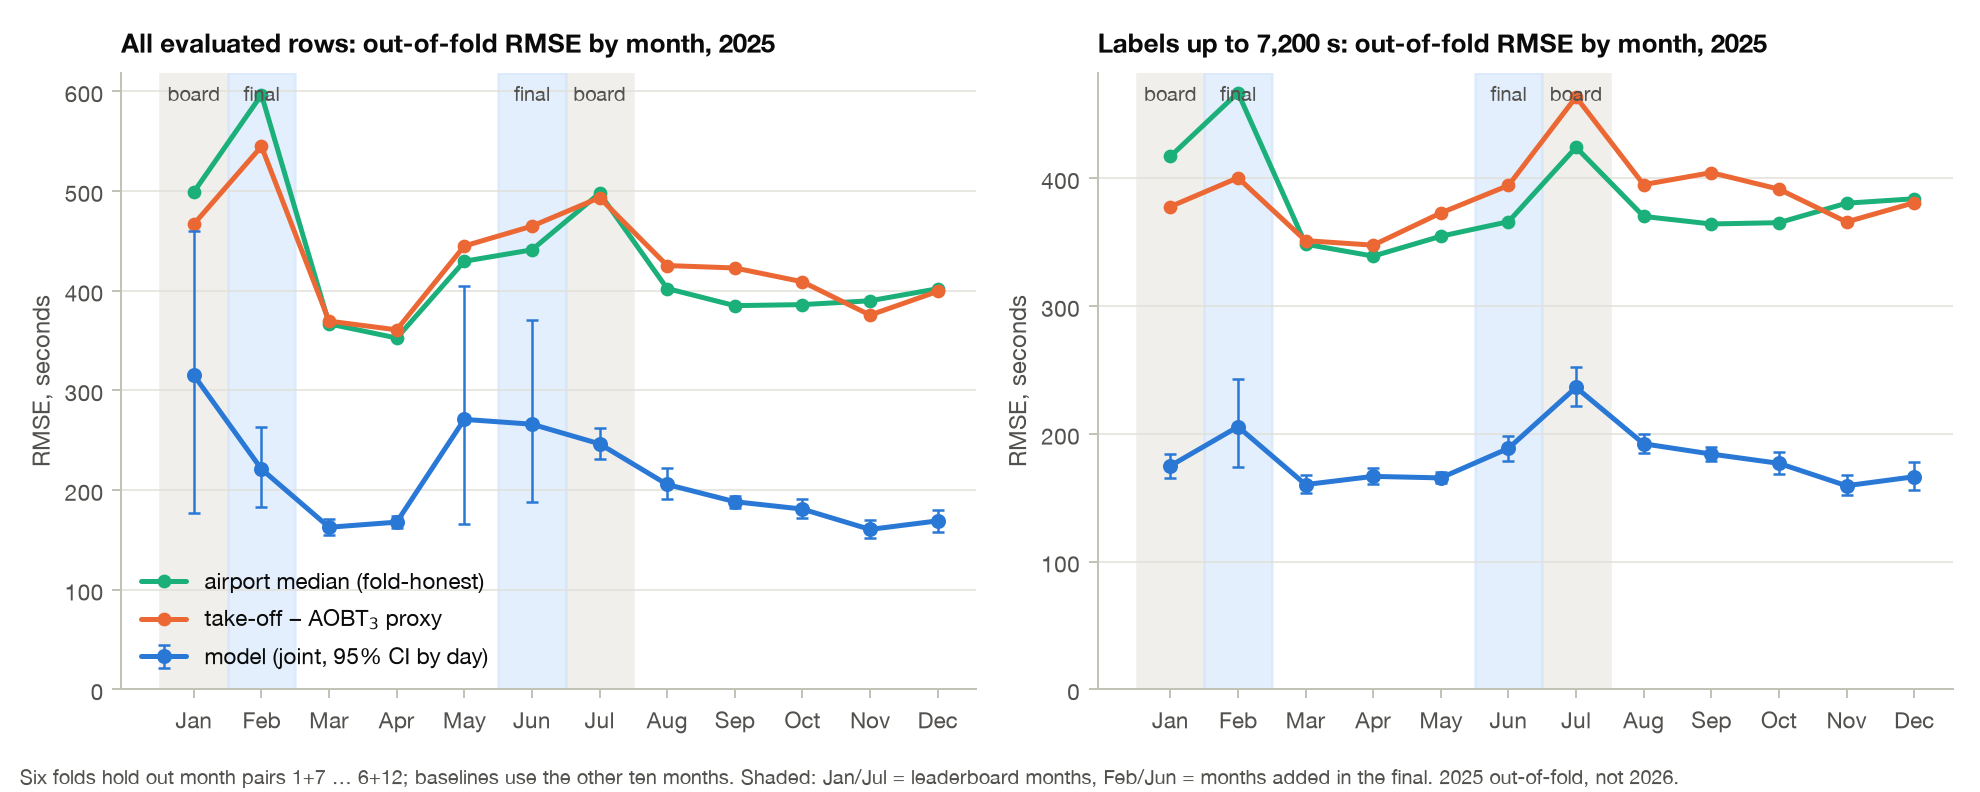
\includegraphics[width=\textwidth]{fig_generalisation_months.png}}
\caption{Out-of-fold RMSE by month for the model and two fold-honest baselines (airport median; take-off minus AOBT\_3), all rows and labels up to 7,200 s.}\label{fig:7}
\end{figure}

The new months were not harder than the leaderboard months in 2025: Feb + Jun minus Jan + Jul is $-$31.9 s on all rows (interval $-$130.3 to +69.0 s) and $-$14.9 s on the body ($-$33.5 to +6.9 s); the intervals include zero, so the difference is not established either. Body RMSE is 159--206 s in eleven months and 236 s in July; February's 206 s is the second highest and is due to one airport, LTFM (417 s against 185--245 s in the other months), which had a snow episode on 19--23 February 2025. All-rows RMSE is driven by single rows in some months: January's 315 s against 175 s on the body comes from two LFPG labels of 23 and 16 hours, June's 266 s against 189 s from one LIRF label of 24 h 13 min. The gain over the baselines does not depend on the month: the body gain over the raw NM proxy is 181--227 s in every month (Jan + Jul 216 s, Feb + Jun 201 s), and in no airport-month (0 of 120) is the model worse than the proxy (Figure~\ref{fig:8}). Across the twelve months, body RMSE moves with the number of labels above two hours (r = +0.89), the share of departures without an NM record (+0.79) and the label standard deviation (+0.67), and against own-track ADS-B coverage ($-$0.45); these are descriptive correlations on twelve points.

\begin{figure}
\centering
\pandocbounded{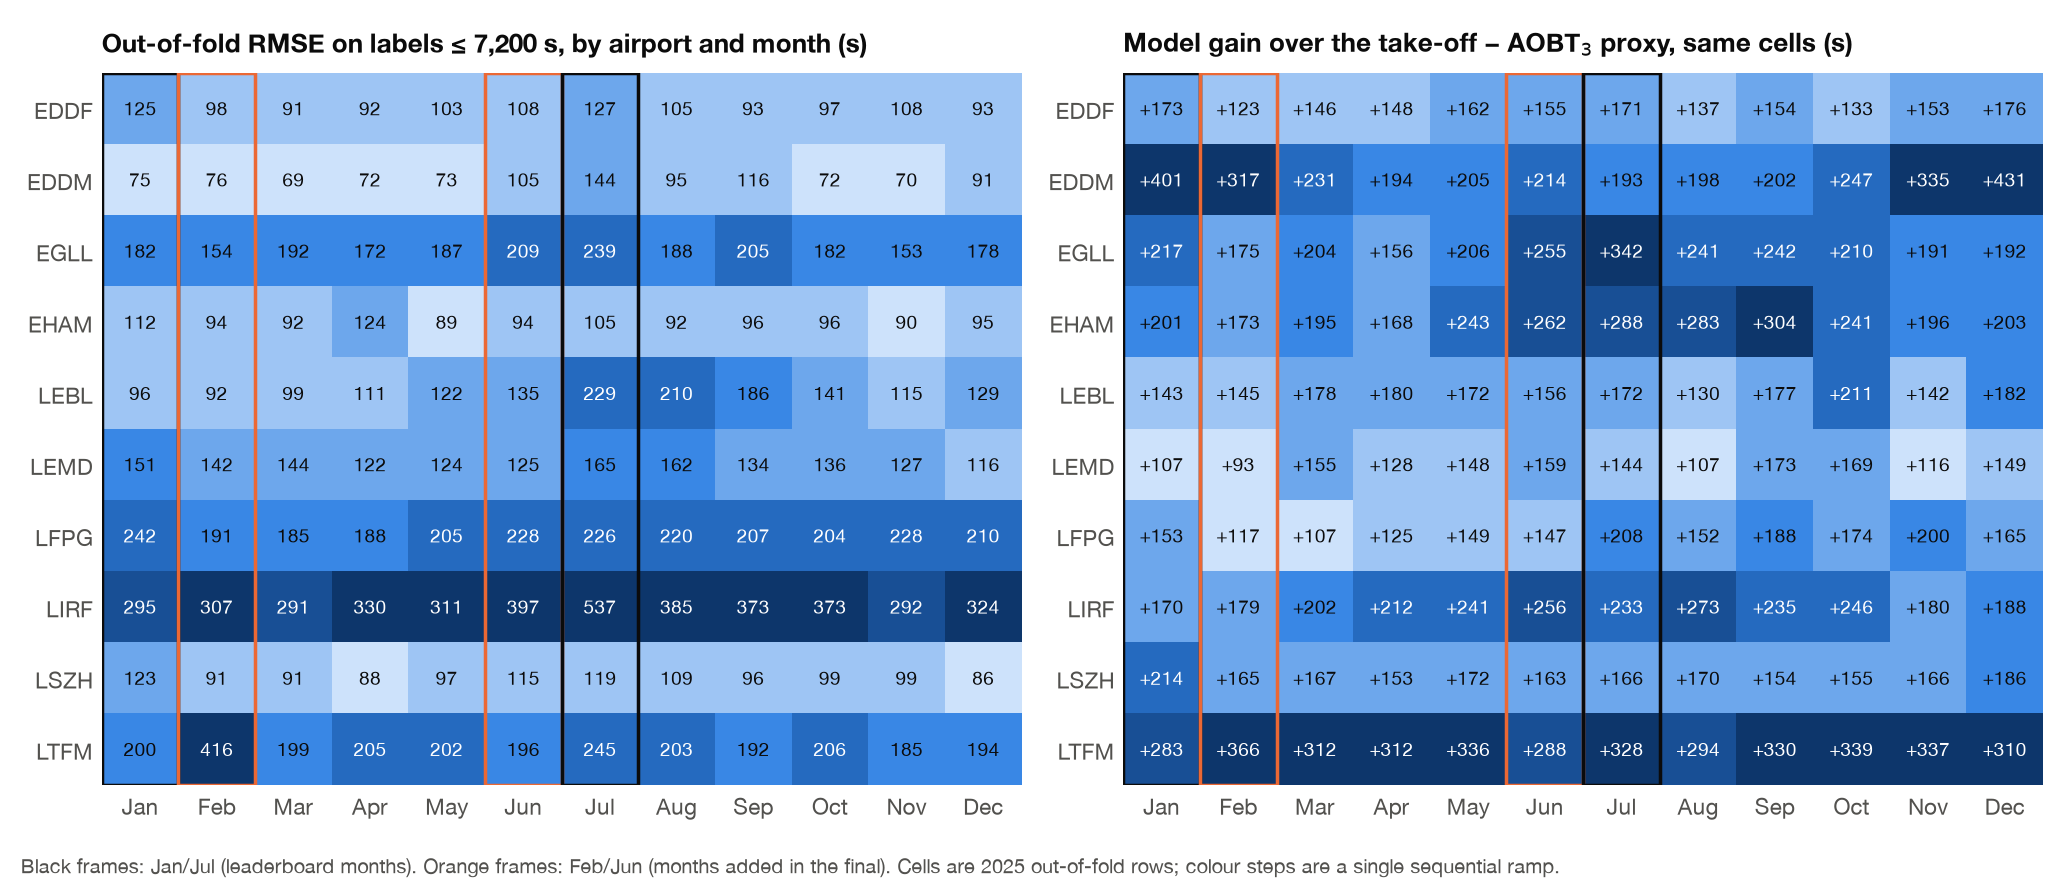
\includegraphics[width=\textwidth]{fig_generalisation_airport_month.png}}
\caption{Body RMSE and gain over the NM proxy by airport and month, 2025 out-of-fold.}\label{fig:8}
\end{figure}

The neural weight of Section 3.4 is the one design parameter chosen after the final was announced, so Table~\ref{tab:10} and Figure~\ref{fig:9} show that it is not tuned to January and July: the per-month optimum ranges from 0.30 to 0.60, January prefers 0.40, and 0.35 is the only grid value below 0.25 in every month, with gains of $-$0.117 s (January), $-$0.675 s (February), $-$0.140 s (June) and $-$0.107 s (July) on 2025 data. February is the outlier: its curve keeps falling up to the largest weight on the grid, while July bottoms out at 0.35 and August at 0.30, so a weight chosen on pooled months would trade the summer for February.

{
\begin{longtable}[]{@{}
  >{\raggedright\arraybackslash}p{(\linewidth - 10\tabcolsep) * \real{0.1304}}
  >{\raggedleft\arraybackslash}p{(\linewidth - 10\tabcolsep) * \real{0.1739}}
  >{\raggedleft\arraybackslash}p{(\linewidth - 10\tabcolsep) * \real{0.1739}}
  >{\raggedleft\arraybackslash}p{(\linewidth - 10\tabcolsep) * \real{0.1739}}
  >{\raggedleft\arraybackslash}p{(\linewidth - 10\tabcolsep) * \real{0.1739}}
  >{\raggedleft\arraybackslash}p{(\linewidth - 10\tabcolsep) * \real{0.1739}}@{}}
\caption{Change of decided-row out-of-fold RMSE against the 0.25 weight, per month of 2025, ten-seed member (E212).}\label{tab:10}\tabularnewline
\toprule\noalign{}
\begin{minipage}[b]{\linewidth}\raggedright
Month
\end{minipage} & \begin{minipage}[b]{\linewidth}\raggedleft
Best weight on the grid
\end{minipage} & \begin{minipage}[b]{\linewidth}\raggedleft
$\Delta$RMSE at 0.35 (s)
\end{minipage} & \begin{minipage}[b]{\linewidth}\raggedleft
at 0.40
\end{minipage} & \begin{minipage}[b]{\linewidth}\raggedleft
at 0.45
\end{minipage} & \begin{minipage}[b]{\linewidth}\raggedleft
at 0.50
\end{minipage} \\
\midrule\noalign{}
\endfirsthead
\caption[]{(continued)}\tabularnewline
\toprule\noalign{}
\begin{minipage}[b]{\linewidth}\raggedright
Month
\end{minipage} & \begin{minipage}[b]{\linewidth}\raggedleft
Best weight on the grid
\end{minipage} & \begin{minipage}[b]{\linewidth}\raggedleft
$\Delta$RMSE at 0.35 (s)
\end{minipage} & \begin{minipage}[b]{\linewidth}\raggedleft
at 0.40
\end{minipage} & \begin{minipage}[b]{\linewidth}\raggedleft
at 0.45
\end{minipage} & \begin{minipage}[b]{\linewidth}\raggedleft
at 0.50
\end{minipage} \\
\midrule\noalign{}
\endhead
\bottomrule\noalign{}
\endlastfoot
Jan & 0.40 & $-$0.117 & $-$0.141 & $-$0.117 & $-$0.077 \\
Feb & 0.60 & $-$0.675 & $-$0.957 & $-$1.172 & $-$1.344 \\
Mar & 0.55 & $-$0.449 & $-$0.595 & $-$0.717 & $-$0.793 \\
Apr & 0.35 & $-$0.108 & $-$0.104 & $-$0.057 & +0.016 \\
May & 0.45 & $-$0.198 & $-$0.249 & $-$0.266 & $-$0.265 \\
Jun & 0.40 & $-$0.140 & $-$0.160 & $-$0.140 & $-$0.093 \\
Jul & 0.35 & $-$0.107 & $-$0.104 & $-$0.049 & +0.051 \\
Aug & 0.30 & $-$0.024 & +0.016 & +0.114 & +0.238 \\
Sep & 0.35 & $-$0.108 & $-$0.100 & $-$0.037 & +0.063 \\
Oct & 0.35 & $-$0.121 & $-$0.116 & $-$0.051 & +0.059 \\
Nov & 0.35 & $-$0.123 & $-$0.123 & $-$0.072 & +0.033 \\
Dec & 0.50 & $-$0.349 & $-$0.441 & $-$0.472 & $-$0.474 \\
Months better than 0.25 & & \textbf{12 of 12} & 11 of 12 & 9 of 12 & 7 of 12 \\
\end{longtable}
}

\begin{figure}
\centering
\pandocbounded{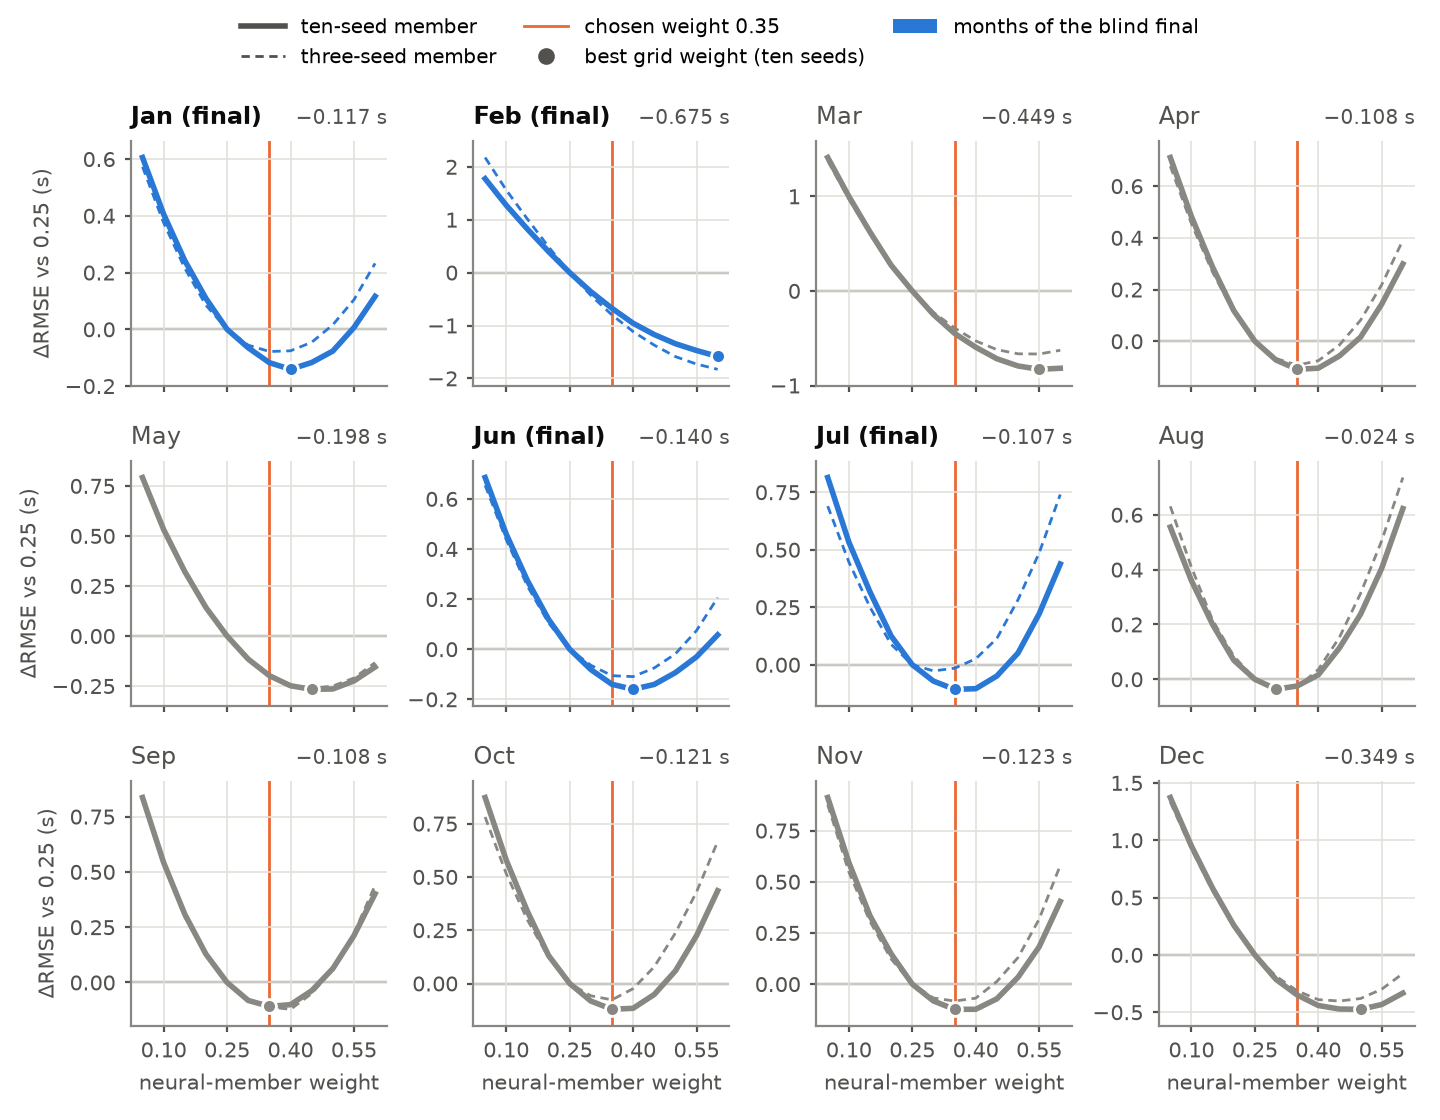
\includegraphics[width=\textwidth]{nn_weight_by_month.png}}
\caption{Change of the decided-row 2025 out-of-fold RMSE of the chain (before the E81 blend) against the neural-member weight, per month, relative to the weight 0.25 of v12075 (E212). Solid: ten-seed member; dashed: three-seed member; dot: best grid weight with ten seeds; vertical line: the chosen 0.35; number above each panel: change at 0.35 with ten seeds. Blue panels are the four months of the blind final. The y-scales differ between panels.}\label{fig:9}
\end{figure}

These are 2025 numbers, not a measurement of 2026. Reading across, the no-NM share of February 2026 (0.91 \%) is close to February 2025 (0.77 \%) and half of January 2026 (1.60 \%), June 2026 (1.35 \%) matches June 2025 (1.36 \%), and LTFM February 2026 shows no snow signature (the share of take-off minus schedule above one hour is 7.2 \% against 12.9 \% in February 2025); the surface coverage of the final months is in Section 2.4.

\subsection{Calibrated uncertainty from the mixture}\label{calibrated-uncertainty-from-the-mixture}

The classifier probabilities and the candidate values define a predictive distribution per flight at no extra training cost: the planned regimes are point masses at their candidates, and the regular regime is the centre plus an empirical residual distribution per airport (99 percentiles of the residual on flights whose true regime is regular, fitted on the other five folds). Two centres were evaluated on the 2,084,921 out-of-fold rows: the base regressor inside the registered mixture, and the value that makes the mixture mean equal the production chain forecast (Table~\ref{tab:11}; Figure~\ref{fig:10}).

{
\begin{longtable}[]{@{}
  >{\raggedright\arraybackslash}p{(\linewidth - 14\tabcolsep) * \real{0.1034}}
  >{\raggedright\arraybackslash}p{(\linewidth - 14\tabcolsep) * \real{0.1034}}
  >{\raggedright\arraybackslash}p{(\linewidth - 14\tabcolsep) * \real{0.1034}}
  >{\raggedleft\arraybackslash}p{(\linewidth - 14\tabcolsep) * \real{0.1379}}
  >{\raggedleft\arraybackslash}p{(\linewidth - 14\tabcolsep) * \real{0.1379}}
  >{\raggedleft\arraybackslash}p{(\linewidth - 14\tabcolsep) * \real{0.1379}}
  >{\raggedleft\arraybackslash}p{(\linewidth - 14\tabcolsep) * \real{0.1379}}
  >{\raggedleft\arraybackslash}p{(\linewidth - 14\tabcolsep) * \real{0.1379}}@{}}
\caption{Calibration of the predictive distribution, 2025 out-of-fold rows.}\label{tab:11}\tabularnewline
\toprule\noalign{}
\begin{minipage}[b]{\linewidth}\raggedright
Variant
\end{minipage} & \begin{minipage}[b]{\linewidth}\raggedright
Coverage 50 / 80 / 90 \%
\end{minipage} & \begin{minipage}[b]{\linewidth}\raggedright
Median width 50 / 80 / 90 \% (s)
\end{minipage} & \begin{minipage}[b]{\linewidth}\raggedleft
CRPS (s)
\end{minipage} & \begin{minipage}[b]{\linewidth}\raggedleft
Point MAE (s)
\end{minipage} & \begin{minipage}[b]{\linewidth}\raggedleft
Climatology CRPS (s)
\end{minipage} & \begin{minipage}[b]{\linewidth}\raggedleft
Skill vs point
\end{minipage} & \begin{minipage}[b]{\linewidth}\raggedleft
Skill vs climatology
\end{minipage} \\
\midrule\noalign{}
\endfirsthead
\caption[]{(continued)}\tabularnewline
\toprule\noalign{}
\begin{minipage}[b]{\linewidth}\raggedright
Variant
\end{minipage} & \begin{minipage}[b]{\linewidth}\raggedright
Coverage 50 / 80 / 90 \%
\end{minipage} & \begin{minipage}[b]{\linewidth}\raggedright
Median width 50 / 80 / 90 \% (s)
\end{minipage} & \begin{minipage}[b]{\linewidth}\raggedleft
CRPS (s)
\end{minipage} & \begin{minipage}[b]{\linewidth}\raggedleft
Point MAE (s)
\end{minipage} & \begin{minipage}[b]{\linewidth}\raggedleft
Climatology CRPS (s)
\end{minipage} & \begin{minipage}[b]{\linewidth}\raggedleft
Skill vs point
\end{minipage} & \begin{minipage}[b]{\linewidth}\raggedleft
Skill vs climatology
\end{minipage} \\
\midrule\noalign{}
\endhead
\bottomrule\noalign{}
\endlastfoot
\texttt{base} (mixture mean, point RMSE 240.16 s) & 49.7 / 79.7 / 89.6 \% & 175 / 365 / 504 & 96.9 & 131.9 & 188.8 & 26.5 \% & 48.7 \% \\
\texttt{chain} (production forecast, point RMSE 218.26 s) & 51.0 / 80.1 / 89.7 \% & 125 / 280 / 396 & 76.5 & 101.8 & 188.8 & 24.9 \% & 59.5 \% \\
\end{longtable}
}

\begin{figure}
\centering
\pandocbounded{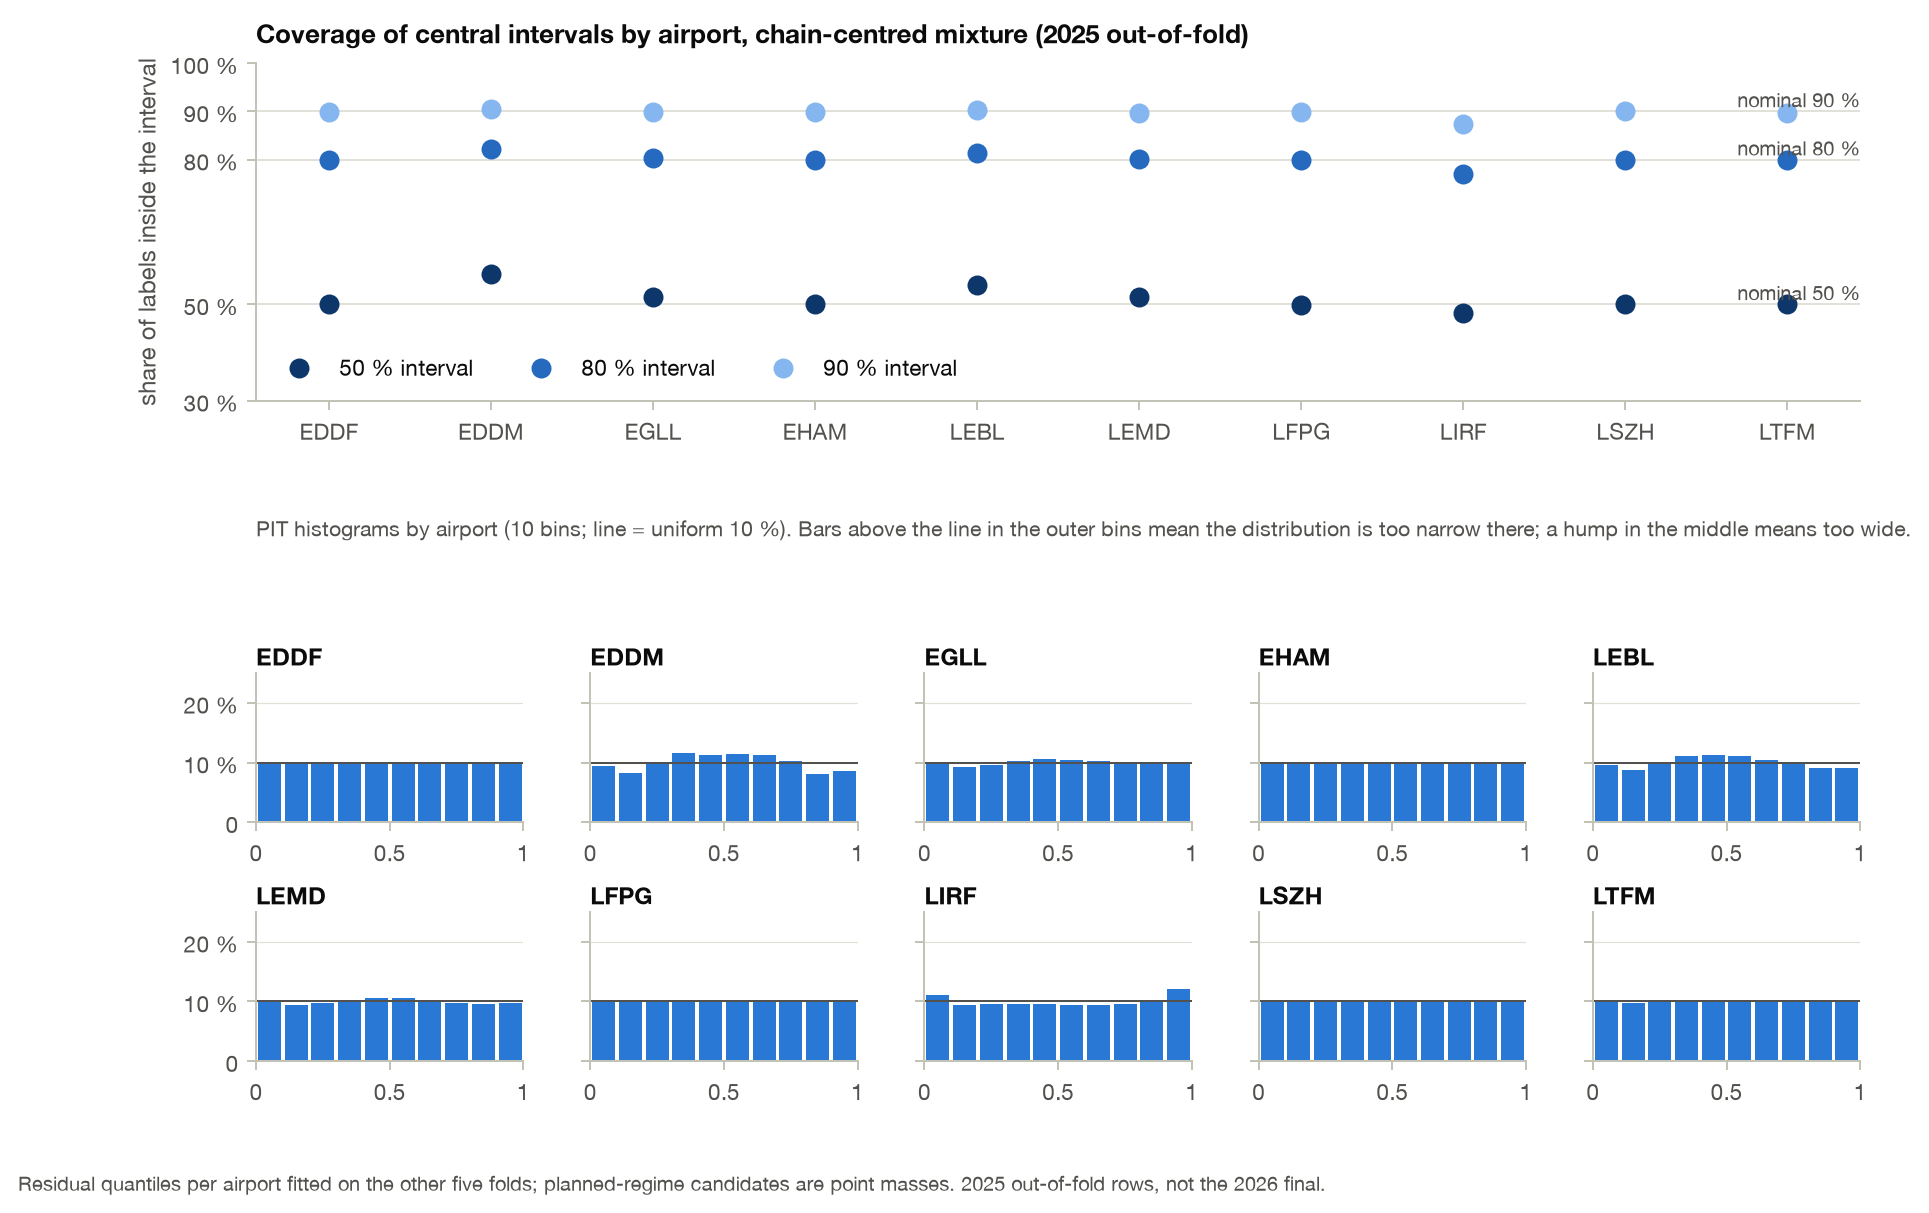
\includegraphics[width=\textwidth]{fig_uncertainty_calibration.png}}
\caption{Coverage of the 50/80/90 \% intervals by airport and probability-integral-transform histograms, chain variant.}\label{fig:10}
\end{figure}

Both variants are calibrated on the whole set to within one point of nominal, with symmetric tails (5.2 \% below the 5 \% quantile, 5.1 \% above the 95 \%); the chain variant is 23 \% sharper at the same coverage. By airport, those with a stable residual spread (EDDF, EHAM, LFPG, LSZH, LTFM) are calibrated to within half a point; EDDM and LEBL are slightly too wide (50 \% interval covers 56 \% and 54 \%) and LIRF too narrow (77 \% and 87 \% for the 80 \% and 90 \% intervals), because a single yearly residual table misses their seasonal spread. By month group the coverage of the 50/80/90 \% intervals is 47.4 / 76.6 / 87.1 \% for Jan + Jul, 51.0 / 80.3 / 89.9 \% for Feb + Jun and 51.9 / 80.9 / 90.3 \% for the other months; July is the only month more than three points below nominal. The one population where the distribution fails is the 22,298 rows without an NM record (coverage 30.3 / 56.6 / 70.7 \%, CRPS 224 s): the mixture has no candidate for a missing planning time. The median of the distribution is not a better point forecast than the mean under RMSE (223.1 s against 218.3 s), as expected for right-skewed residuals.

\subsection{The regime classifier as a data-quality detector, and the PRU view}\label{the-regime-classifier-as-a-data-quality-detector-and-the-pru-view}

The detector is \(P(\text{planning copy}) = 1 - P(\text{regular})\), out of fold, evaluated against the $\pm$6 s label rule (Figure~\ref{fig:11}). Over the seven labelled airports the mean probability is 9.46 \% against a label share of 9.58 \%; the expected number of copies is 139,319 against 140,992 labels ($-$1.2 \%), and per airport the two agree within 0.1 percentage point (LIRF 23.91 \% against 24.14 \%). The reliability curve follows the diagonal across the whole range (bin {[}0.50, 0.60): 0.548 against 0.547; bin {[}0.99, 1{]}: 0.994 against 0.999); at the three airports without planned-regime labels the detector is quiet (5--9 expected copies in 135,000--248,000 departures). Brier score 0.075 on the labelled airports. Individual flags are confident only at LIRF: AUC against the rule is 0.795, and of the flags at \(P \ge 0.5\) (precision 71.1 \%, recall 8.8 \%) 17,361 of 17,424 are at LIRF; at \(P \ge 0.95\) precision is 99.2 \% (Table~\ref{tab:12}). The detector does not try to call the coincidental copies, because a coincidental copy costs the mixture nothing. The expected count is therefore a usable monthly statistic at every labelled airport, while the per-flight flag is usable at LIRF and, elsewhere, only above about 0.8, where it almost never fires.

\begin{figure}
\centering
\pandocbounded{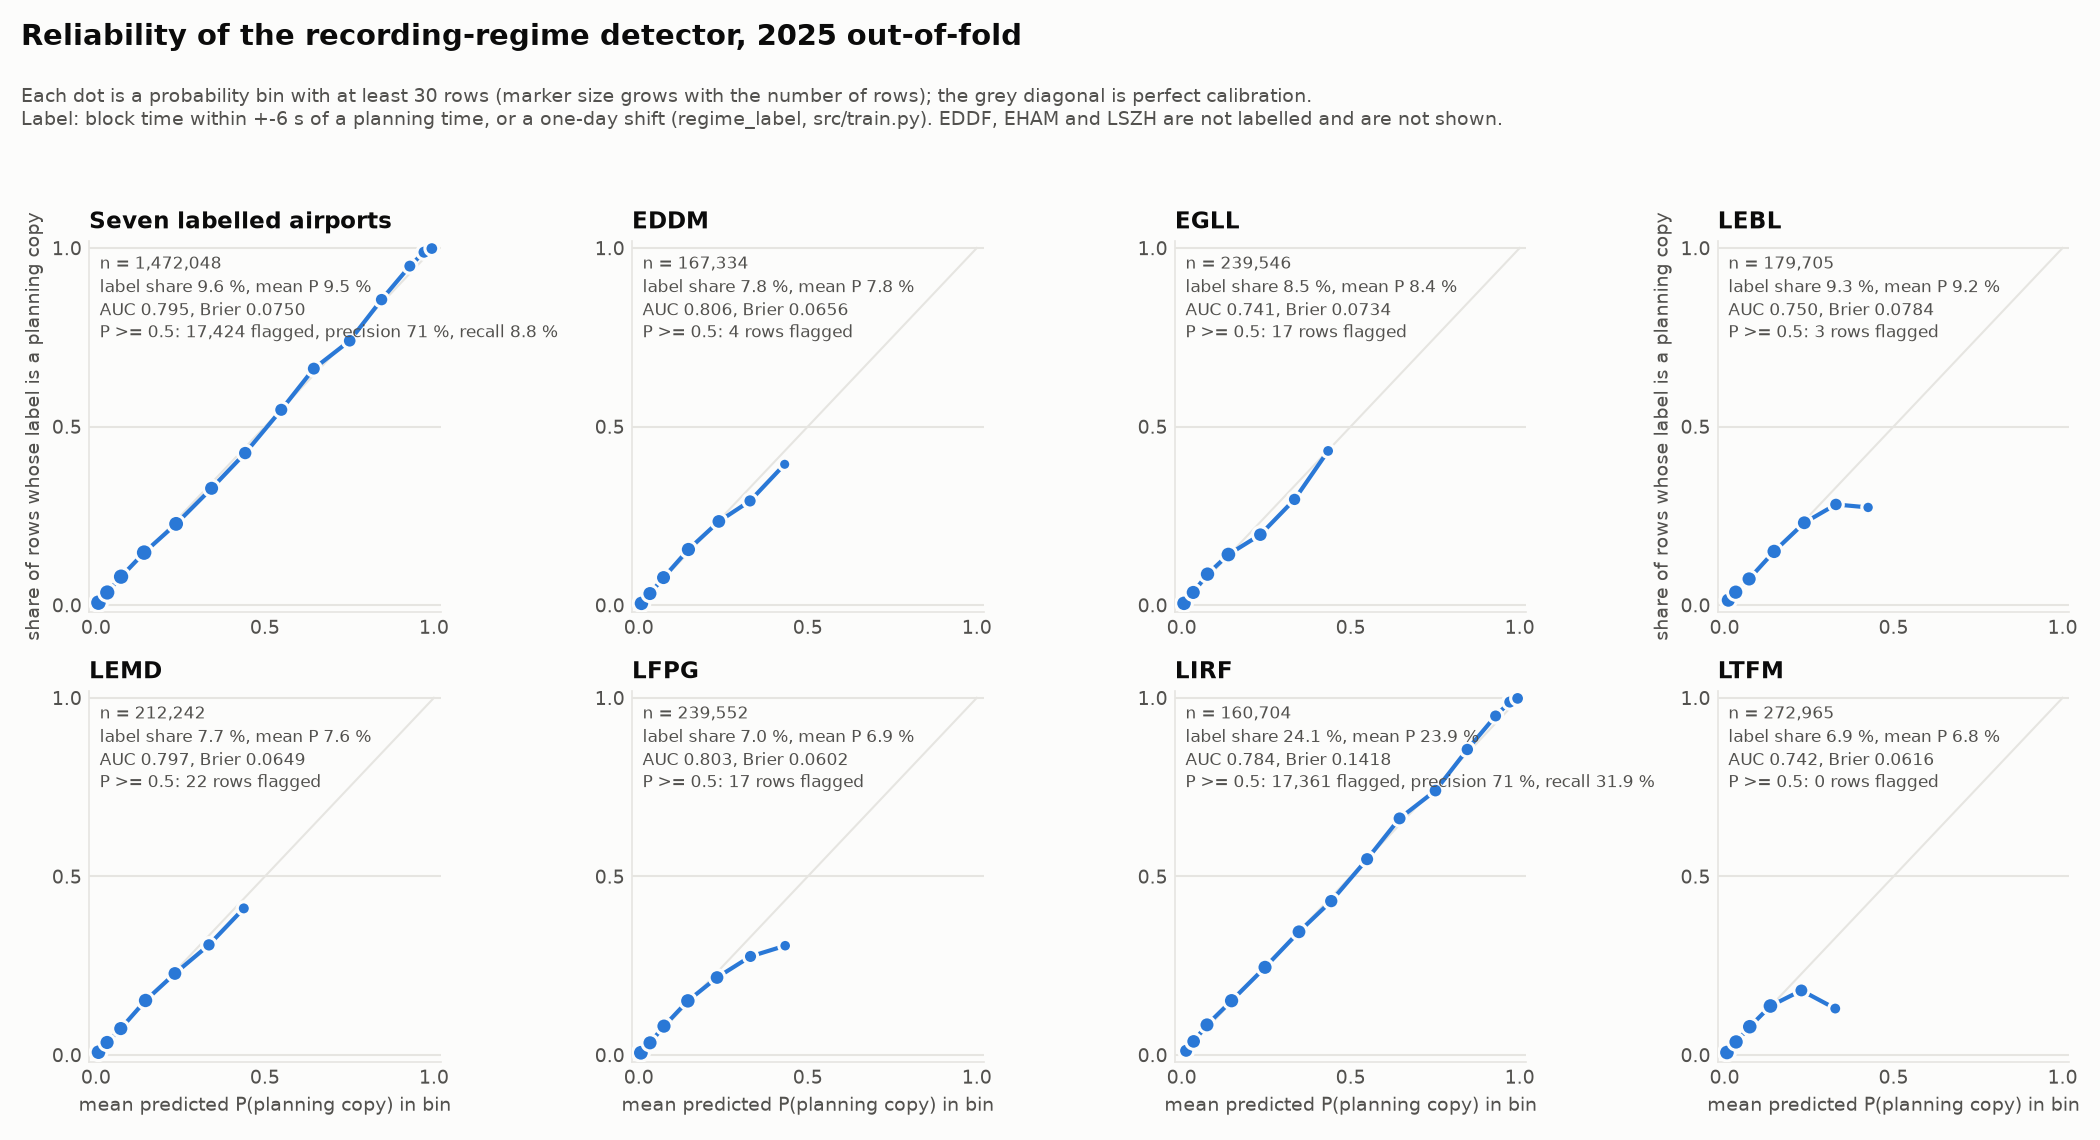
\includegraphics[width=\textwidth]{fig6_regime_detector_calibration.png}}
\caption{Reliability diagrams of the detector, seven labelled airports together and per airport.}\label{fig:11}
\end{figure}

{
\begin{longtable}[]{@{}
  >{\raggedleft\arraybackslash}p{(\linewidth - 8\tabcolsep) * \real{0.2000}}
  >{\raggedleft\arraybackslash}p{(\linewidth - 8\tabcolsep) * \real{0.2000}}
  >{\raggedleft\arraybackslash}p{(\linewidth - 8\tabcolsep) * \real{0.2000}}
  >{\raggedleft\arraybackslash}p{(\linewidth - 8\tabcolsep) * \real{0.2000}}
  >{\raggedleft\arraybackslash}p{(\linewidth - 8\tabcolsep) * \real{0.2000}}@{}}
\caption{Precision and recall of the flag \(P \ge t\) against the $\pm$6 s rule, 2025 out of fold.}\label{tab:12}\tabularnewline
\toprule\noalign{}
\begin{minipage}[b]{\linewidth}\raggedleft
Threshold
\end{minipage} & \begin{minipage}[b]{\linewidth}\raggedleft
Flagged
\end{minipage} & \begin{minipage}[b]{\linewidth}\raggedleft
Precision
\end{minipage} & \begin{minipage}[b]{\linewidth}\raggedleft
Recall (all labelled airports)
\end{minipage} & \begin{minipage}[b]{\linewidth}\raggedleft
Recall at LIRF
\end{minipage} \\
\midrule\noalign{}
\endfirsthead
\caption[]{(continued)}\tabularnewline
\toprule\noalign{}
\begin{minipage}[b]{\linewidth}\raggedleft
Threshold
\end{minipage} & \begin{minipage}[b]{\linewidth}\raggedleft
Flagged
\end{minipage} & \begin{minipage}[b]{\linewidth}\raggedleft
Precision
\end{minipage} & \begin{minipage}[b]{\linewidth}\raggedleft
Recall (all labelled airports)
\end{minipage} & \begin{minipage}[b]{\linewidth}\raggedleft
Recall at LIRF
\end{minipage} \\
\midrule\noalign{}
\endhead
\bottomrule\noalign{}
\endlastfoot
0.50 & 17,424 & 71.1 \% & 8.8 \% & 31.9 \% \\
0.80 & 4,768 & 92.8 \% & 3.1 \% & 11.4 \% \\
0.95 & 1,871 & 99.2 \% & 1.3 \% & 4.8 \% \\
\end{longtable}
}

To see what the copies do to a monitoring statistic, we emulated the PRU additional-taxi-out indicator from the challenge records: taxi-out minus an unimpeded reference, the 10th percentile per stand $\times$ departure-runway group over 2025, valid with at least ten flights at or below it, after PRU's filters (deviations forced by the data: calendar-year instead of rolling window, UTC months, no de-icing exclusion, 41 helicopter designators excluded). Against the published 2025 indicator for April--October (70 airport-months) the emulation has a mean absolute difference of 3.3 s, median 1.8 s, maximum 14.5 s and correlation 0.999; November--March the difference grows to 25.7 s with a +23.5 s bias, which is the de-icing exclusion we cannot apply (PRU removes 20--31 \% of EDDM's winter departures). The agreement also shows that the published indicator is computed from the same records, planning copies included. The indicator was then computed three ways: as recorded, with the rule-labelled copies removed, and with every record weighted by \(P(\text{regular})\) (Table~\ref{tab:13}; Figure~\ref{fig:12}).

{
\begin{longtable}[]{@{}
  >{\raggedright\arraybackslash}p{(\linewidth - 10\tabcolsep) * \real{0.1304}}
  >{\raggedleft\arraybackslash}p{(\linewidth - 10\tabcolsep) * \real{0.1739}}
  >{\raggedleft\arraybackslash}p{(\linewidth - 10\tabcolsep) * \real{0.1739}}
  >{\raggedleft\arraybackslash}p{(\linewidth - 10\tabcolsep) * \real{0.1739}}
  >{\raggedleft\arraybackslash}p{(\linewidth - 10\tabcolsep) * \real{0.1739}}
  >{\raggedleft\arraybackslash}p{(\linewidth - 10\tabcolsep) * \real{0.1739}}@{}}
\caption{Effect of planning-copy records on the emulated additional-taxi-out indicator, 2025 per airport, seconds per flight (positive: the as-recorded value is higher).}\label{tab:13}\tabularnewline
\toprule\noalign{}
\begin{minipage}[b]{\linewidth}\raggedright
Airport
\end{minipage} & \begin{minipage}[b]{\linewidth}\raggedleft
Copies (rule / detector)
\end{minipage} & \begin{minipage}[b]{\linewidth}\raggedleft
Indicator as recorded
\end{minipage} & \begin{minipage}[b]{\linewidth}\raggedleft
Rule-cleaned (A $-$ B)
\end{minipage} & \begin{minipage}[b]{\linewidth}\raggedleft
Probability-cleaned (A $-$ C)
\end{minipage} & \begin{minipage}[b]{\linewidth}\raggedleft
Largest monthly A $-$ B
\end{minipage} \\
\midrule\noalign{}
\endfirsthead
\caption[]{(continued)}\tabularnewline
\toprule\noalign{}
\begin{minipage}[b]{\linewidth}\raggedright
Airport
\end{minipage} & \begin{minipage}[b]{\linewidth}\raggedleft
Copies (rule / detector)
\end{minipage} & \begin{minipage}[b]{\linewidth}\raggedleft
Indicator as recorded
\end{minipage} & \begin{minipage}[b]{\linewidth}\raggedleft
Rule-cleaned (A $-$ B)
\end{minipage} & \begin{minipage}[b]{\linewidth}\raggedleft
Probability-cleaned (A $-$ C)
\end{minipage} & \begin{minipage}[b]{\linewidth}\raggedleft
Largest monthly A $-$ B
\end{minipage} \\
\midrule\noalign{}
\endhead
\bottomrule\noalign{}
\endlastfoot
EDDM & 7.8 \% / 7.8 \% & 232.0 & $-$1.7 & $-$4.1 & +0.1 \\
EGLL & 8.5 \% / 8.4 \% & 388.5 & $-$2.8 & $-$5.3 & $-$1.1 \\
LEBL & 9.3 \% / 9.2 \% & 230.9 & +7.3 & $-$2.8 & +26.3 (July) \\
LEMD & 7.7 \% / 7.6 \% & 217.6 & +0.8 & $-$2.3 & +2.1 \\
LFPG & 7.0 \% / 6.9 \% & 271.9 & $-$2.0 & $-$4.4 & +0.7 \\
LIRF & 24.1 \% / 23.9 \% & 400.6 & +42.1 & +6.2 & +66.7 (July) \\
LTFM & 6.9 \% / 6.8 \% & 294.2 & +1.1 & $-$1.3 & +15.5 (February) \\
\end{longtable}
}

\begin{figure}
\centering
\pandocbounded{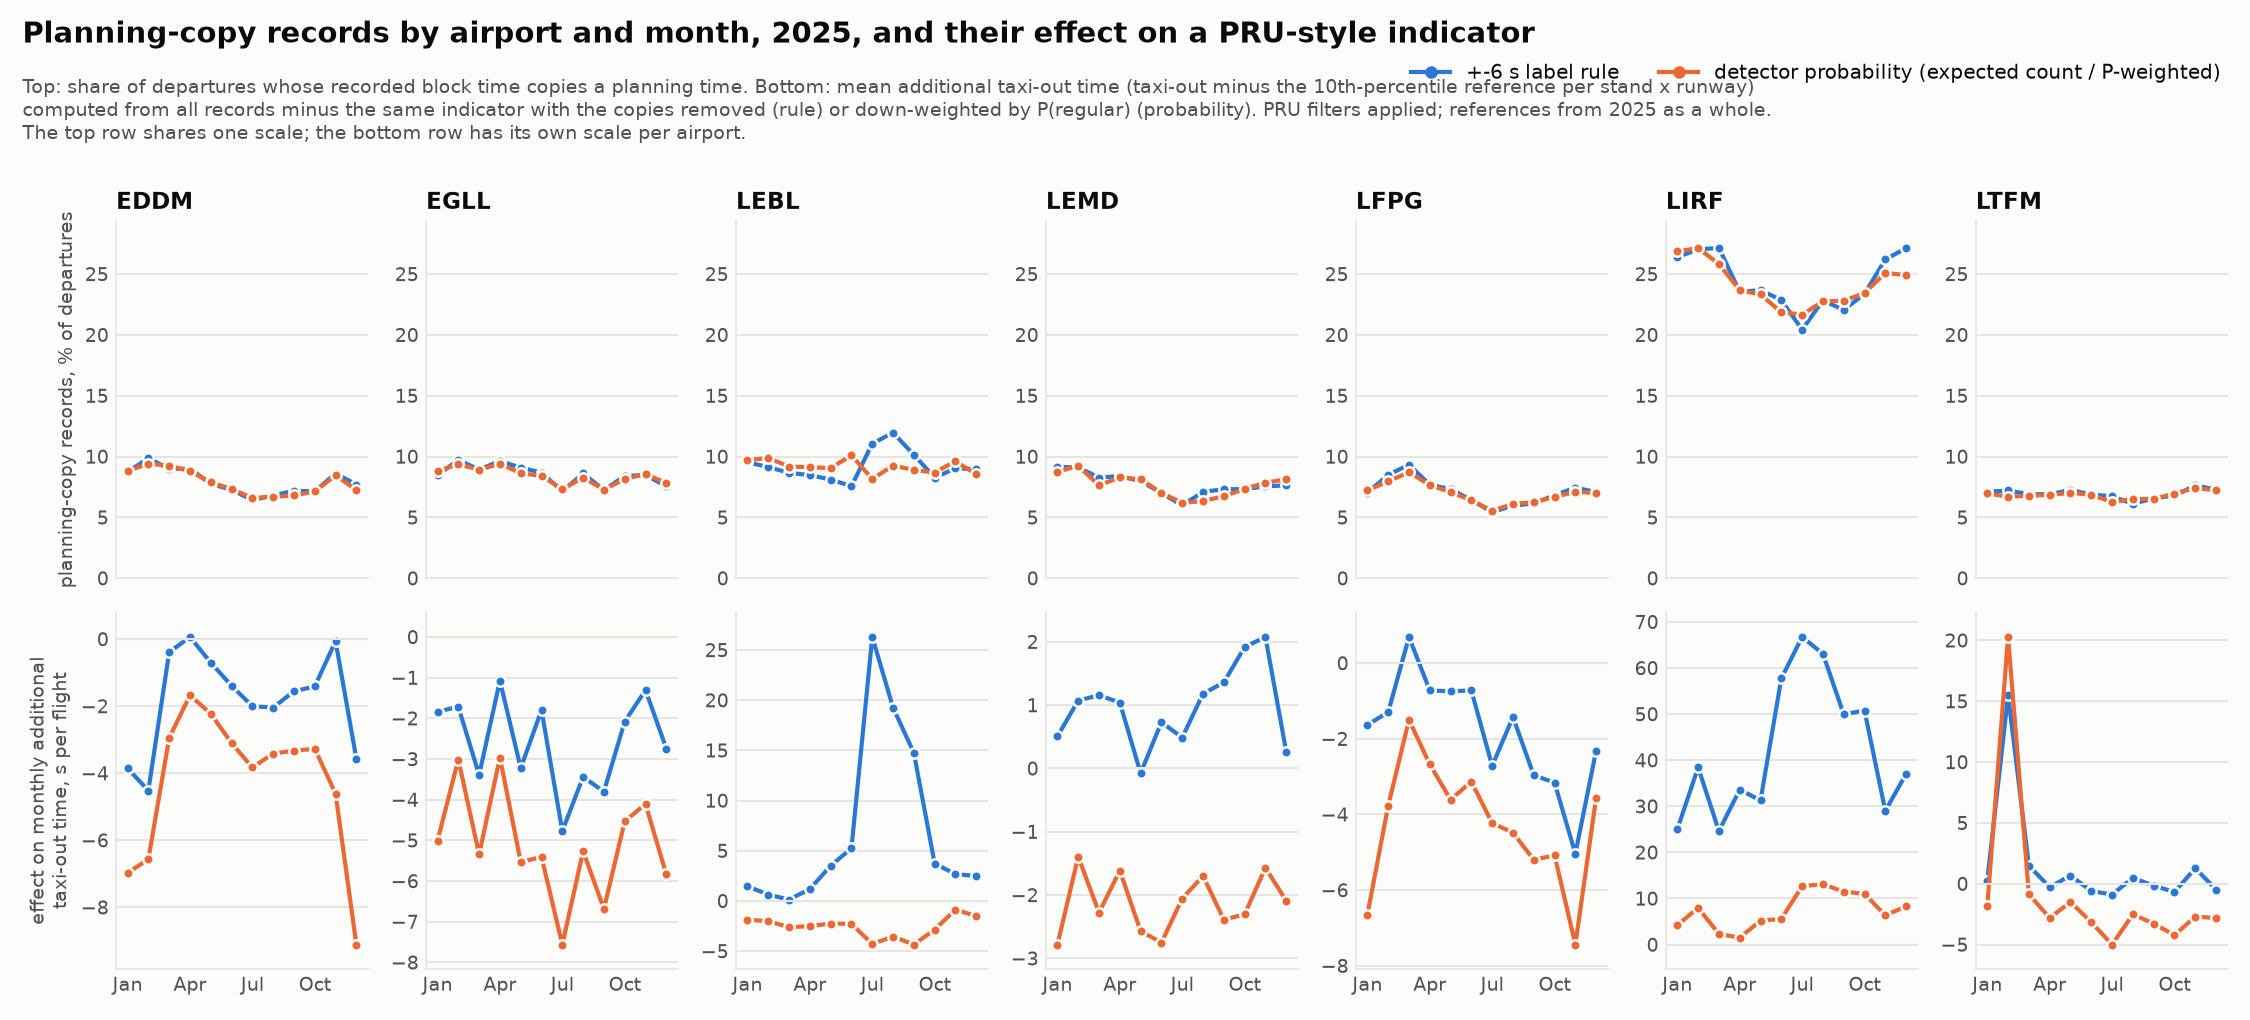
\includegraphics[width=\textwidth]{fig7_regime_effect_on_kpi.png}}
\caption{Monthly share of planning-copy departures per airport (rule and detector) and the effect of those records on the monthly indicator.}\label{fig:12}
\end{figure}

Outside LIRF the copies do not inflate the statistics: the annual effect is between $-$2.8 and +1.1 s per flight by the rule, and negative by probability (labelled records are slightly shorter than the rest, as on-time departures are), with two episodes worth a monitoring unit's attention: LEBL in July--September 2025 (+26, +19, +15 s per flight by the rule; the label share rose to 11.9--12.3 \% while the detector, trained on the other months, stayed at 8--9 \%, which looks like a change in how delayed departures were recorded) and LTFM in February 2025 (+15 s). At LIRF the copies are the dominant data-quality issue: the PRU-style indicator is 25--67 s per flight higher by the rule (largest in June--August) and 1.5--13 s by the probability lower bound; for an annual value of 401 s the rule-based effect is about 10 \%. The reference itself is barely affected (7.2 s mean absolute change at LIRF, below 5 s elsewhere).

Read in PRU terms, a taxi-out prediction decomposes as reference plus predicted additional time. On the 1,788,520 regular-regime departures with a valid reference the unimpeded reference is 518--978 s by airport and the additional time averages 196--391 s with a standard deviation of 222--391 s; the chain explains 45--69 \% of its variance beyond the airport-month level (correlation 0.68--0.83). The regular regressor is unbiased on the regular regime at every airport (\textbar bias\textbar{} $\le$ 1.9 s), whereas the mixture is biased upward where copies are frequent (+36.8 s at LIRF, +10.6 s at LEBL): on a row that might be a copy the squared-error optimum moves part of the way towards the planning candidate, and on the rows that turn out regular that move is a positive error. A monthly indicator computed from the predictions reproduces the one computed from the labels within 6.4 s on average over 120 airport-months (bias +0.4 s, correlation 0.994) against a month-to-month spread of 71--77 s. For a PRU-style reading of the regular regime, the regressor, not the mixture, is the right output. Section 5.7 applies the same emulation to the final file's predictions for the four months of 2026 and compares it with the indicator EUROCONTROL has published since.

\subsection{The blind final: recipe cost, file, control and label-free checks}\label{the-blind-final-recipe-cost-file-control-and-label-free-checks}

\textbf{Price of the recipe on January/July.} The uniform recipe was run on the v12075-era January/July artifacts (old members, the three-seed neural member at 0.25, the blend removed, fresh tail rows) and uploaded once as a technical canary, v12090: 232.1933 s against 230.9387 s for v12075, +1.2546 s, inside the forecast corridor {[}231.1; 232.3{]} written before the upload. The canary removed the blend and replaced the 42 donor rows at the same time, so it does not identify either effect alone. On 9 October the two parts were priced on the v12077 chain by single uploads, each the only change against v12077 and each with a forecast written beforehand (Table~\ref{tab:14}; Figure~\ref{fig:13}a). Skipping the blend (v12078) costs +0.5676 s (231.0488 s; corridor {[}230.40; 231.20{]}). Replacing the 42 frozen rows by the fresh ten-seed ensemble (v12079; exactly 42 rows changed, RMS 713.5 s between the two sets of values) costs +0.6958 s (231.1770 s; forecast 231.17, corridor {[}230.83; 231.48{]}). v12079 was uploaded during an outage of the organiser's scorer, which processed no team's file between 08:54:51 and 16:28 UTC, and was scored after the repair, 0.007 s from its central forecast. The two parts add to +1.2634 s against the canary's +1.2546 s, which was measured with the older weights and the three-seed member; the interaction is about $-$0.009 s. The cost of the uniform recipe on January/July is therefore measured, not inferred: about +0.57 s for dropping the blend and +0.70 s for replacing one favourable TabPFN draw by a repeatable ensemble.

{
\begin{longtable}[]{@{}
  >{\raggedright\arraybackslash}p{(\linewidth - 6\tabcolsep) * \real{0.2143}}
  >{\raggedright\arraybackslash}p{(\linewidth - 6\tabcolsep) * \real{0.2143}}
  >{\raggedleft\arraybackslash}p{(\linewidth - 6\tabcolsep) * \real{0.2857}}
  >{\raggedleft\arraybackslash}p{(\linewidth - 6\tabcolsep) * \real{0.2857}}@{}}
\caption{The price of the final recipe on the January/July rows, measured by single uploads.}\label{tab:14}\tabularnewline
\toprule\noalign{}
\begin{minipage}[b]{\linewidth}\raggedright
File
\end{minipage} & \begin{minipage}[b]{\linewidth}\raggedright
What it is
\end{minipage} & \begin{minipage}[b]{\linewidth}\raggedleft
RMSE (s)
\end{minipage} & \begin{minipage}[b]{\linewidth}\raggedleft
Change (s)
\end{minipage} \\
\midrule\noalign{}
\endfirsthead
\caption[]{(continued)}\tabularnewline
\toprule\noalign{}
\begin{minipage}[b]{\linewidth}\raggedright
File
\end{minipage} & \begin{minipage}[b]{\linewidth}\raggedright
What it is
\end{minipage} & \begin{minipage}[b]{\linewidth}\raggedleft
RMSE (s)
\end{minipage} & \begin{minipage}[b]{\linewidth}\raggedleft
Change (s)
\end{minipage} \\
\midrule\noalign{}
\endhead
\bottomrule\noalign{}
\endlastfoot
v12075 & best of 7 October & 230.9387 & --- \\
v12090 & v12075 chain, blend removed, fresh tail rows (canary) & 232.1933 & +1.2546 vs v12075 \\
v12076 & v12075 with the ten-seed neural member & 230.8183 & $-$0.1204 vs v12075 \\
v12077 & v12076 with the 0.35 weight (best) & 230.4812 & $-$0.3371 vs v12076 \\
v12078 & v12077 without the blend & 231.0488 & +0.5676 vs v12077 \\
v12079 & v12077 with fresh tail rows instead of the 42 frozen rows & 231.1770 & +0.6958 vs v12077 \\
H & v12078 with the 42 fresh rows of v12079; not uploaded, exact by the Gram identity (Section 4.4) & 231.7429 & +1.2617 vs v12077 \\
v12080 & January/July rows of the final file (control) & 231.1805 & $-$0.5624 vs H \\
\end{longtable}
}

\begin{figure}
\centering
\pandocbounded{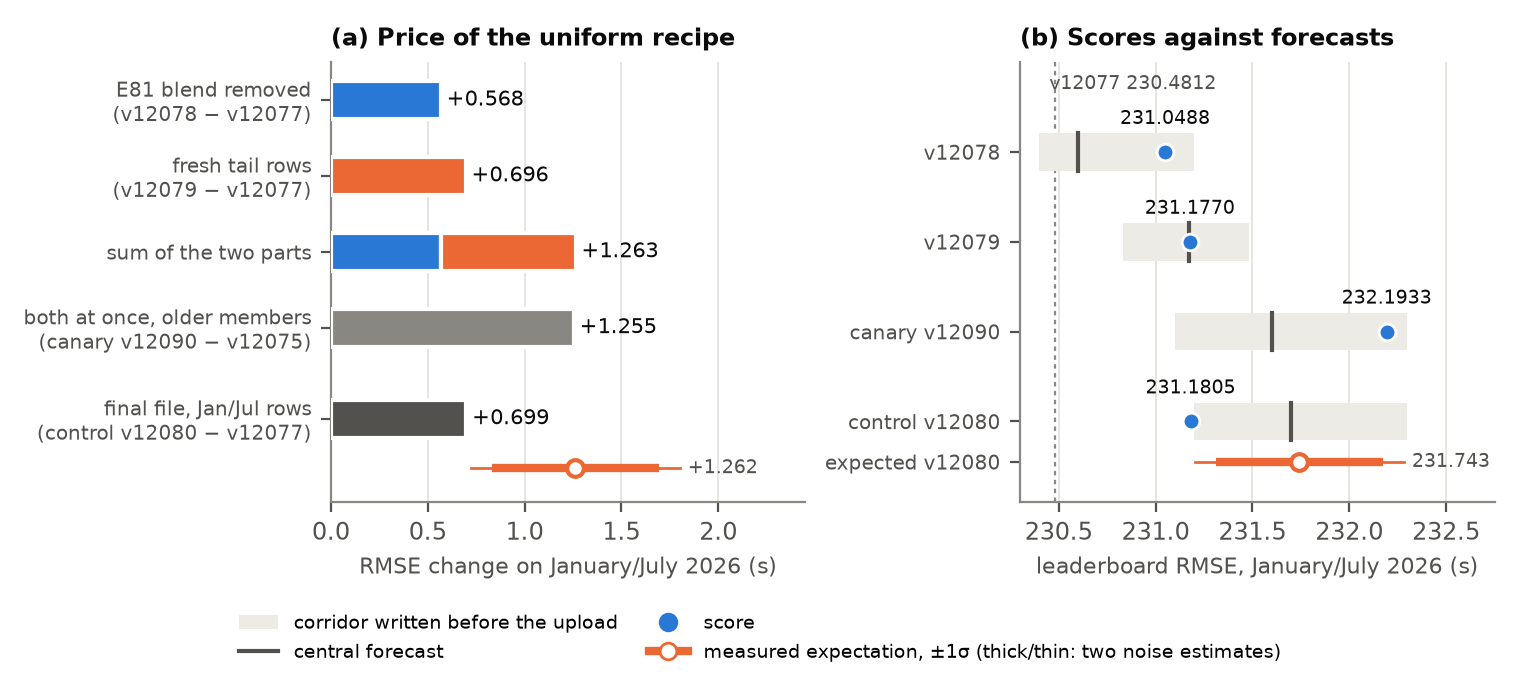
\includegraphics[width=\textwidth]{final_recipe_price.png}}
\caption{The price of the uniform final recipe on January/July 2026, measured by single uploads. (a) Change of each measurement upload against its parent file; the two separately priced parts add to +1.263 s, the canary removed both at once with the older members, and the control is the January/July rows of the final file; the open marker is the expectation H with the two label-free one-sigma noise estimates of the control analysis (thick and thin bar). (b) Each upload against the corridor (band) and central forecast (tick) written before it; v12080 fell 0.02 s below its corridor.}\label{fig:13}
\end{figure}

\textbf{The file.} \texttt{gentle-igloo\_\allowbreak{}final.parquet} was assembled on 9 October 2026 on a single workstation in 157.6 s with zero fits (SHA-256 \texttt{76c32426d750040690ff68bacd6ecbf3a7aa1e63340df5b9271a324b7064d554}, 2,145,126 bytes, 670,790 rows, template SHA \texttt{b3445d80\ldots{}}, ranking file SHA \texttt{4b0692a7\ldots{}}, git commit \texttt{2d85c07a}). The tail stage served 62 rows, with the ten TabPFN seeds bitwise identical on a second run; the blend was not applied and no donor row was copied. The validator passed every hard check (file name, columns and dtypes as in the template, 670,790 rows, identical ID set, no duplicates, no null/NaN/inf, values 0--110,578 s, integer seconds); the file has a mean of 1,012 s, a median of 939 s, 152 values above 7,200 s and 46 zeros. Against v12077 on the 344,841 January/July IDs, 95.6 \% of rows differ with RMS 26.5 s and a maximum of 2,926 s, which is the refit of the members on the four-month view plus the new dithering of the inputs (an RMS of exactly zero would have meant copied rows). An independent second assembly from the same contract (new \texttt{prepare} and \texttt{assemble}, 112.7 s) reproduced the same SHA. Per month $\times$ airport medians lie between 702 s (EHAM June) and 1,331 s (EGLL June); the share of predictions equal to take-off minus a planning time within $\pm$15 s is 2.4--2.8 \% (schedule) to 5.7--6.1 \% (\texttt{AOBT\_\allowbreak{}3}) in every month, with February and June inside the January/July range, so the regime mixture of the new months is not different in kind.

\textbf{Control.} The January/July rows of the final file were sealed as a regular submission (v12080, SHA \texttt{ae1680cb\ldots{}}, 344,841 rows) with a forecast written before the upload: 231.7 s, corridor {[}231.2; 232.3{]} s, derived two ways (v12077 plus the measured blend price plus about +0.6 s for the fresh tail rows; the canary minus the measured $-$0.4575 s of the two member changes), plus $\pm$0.3 s for the refit of the members and the new input dithering. The rule registered with it: a result outside the corridor stops the final upload until a stage-by-stage comparison explains it, and no choice between control files will be made. Once v12079 was scored, the measured decomposition put the expectation at 231.745 s, inside the corridor.

v12080 scored \textbf{231.1805 s}: 0.02 s below the corridor, on the favourable side, and 0.56 s better than the measured expectation (Figure~\ref{fig:13}b). The final upload was paused, as the rule required. Label leakage was excluded first: in the final ranking file the departure block-time and taxi-time fields are null in all four months, as in the ordinary ranking file. The deviation was then decomposed without labels and without fits. The reference is the real file H of Table~\ref{tab:14}; the final rows F differ from it by RMS 20.36 s on 325,612 rows, a change of $-$260.3 s\textsuperscript{2} in mean squared error. Each group of inputs was swapped back to its v12077-era version one at a time and run through the frozen final chain, whose identity run reproduces all twelve stages byte for byte. Projected on F $-$ H, the regime probabilities of the base classifier carry 55 \% of the difference (the classifier was refitted on the four-month view, whose label-free route medians of the \texttt{plan\_\allowbreak{}*} features are taken over four months, and it reads the re-dithered January/July inputs), the neural member 23 \%, the tabular members 16 \%, the rebuilt daily ADS-B products 2 \% and the 42 tail rows 0.4 \%; joint swaps close the decomposition at 99.9 \%. The difference is concentrated: 345 rows (0.1 \%) carry 61.7 \% of its squared size and LIRF in July alone 53.5 \%. On these rows the prediction mixes regime candidates whose median spread is 2,818 s, and 87 \% of the change comes from the probabilities; a typical row is a LIRF July departure without an NM record whose schedule-copy probability moved from 0.79 to 0.55, which moved the prediction from 10,822 s to 7,854 s. Nothing pointed to an error: the members show the same seed spread as before (CatBoost 32.6 s against 32.6 s), the classifier has the same parameters, trees, features and training rows, and the surface stages serve almost the same rows (E141 222,740 against 222,660). Calibrated without labels on the 2025 January + July out-of-fold predictions, the noise of such a control is $\sigma$ $\approx$ 200--250 s\textsuperscript{2} in mean squared error, that is $\pm$0.43--0.55 s in RMSE (1$\sigma$); the observed deviation is a 1.0--1.3$\sigma$ event, and the members alone ($\sigma$ $\approx$ 10--15 s\textsuperscript{2}) could not have produced it. The recipe was not changed and the file remained the only final candidate.

The lesson concerns the forecast, not the model. The corridor allowed $\pm$0.3 s for the refit and the dithering, about half the noise measured afterwards: the $\pm$0.08 s dithering estimate of Section 2.1 holds for a fixed chain, and it does not cover the refitted classifier's response to new inputs, which alone carries about 0.29 s. A control of a chain whose members and classifier are refitted needs a corridor of about $\pm$0.5 s per standard deviation. The same draw is not guaranteed to fall with the same sign on the blind months.

\textbf{Label-free checks of the blind months.} EUROCONTROL publishes the monthly additional-taxi-out indicator per airport; the 2026 file covers January--July \autocite{eurocontrol2026atxotdata}. We computed the indicator from the final file's predictions with the emulation of Section 5.6 (2025 reference per stand $\times$ runway group) and compared it with the published values for the 40 airport-months of the final; the published file is a reference here, not a model input. In summer the two agree: June mean absolute difference 9.2 s (bias $-$1.1 s), July 6.6 s (bias +1.3 s), against 6.6 and 8.2 s for the same procedure applied to the 2025 out-of-fold predictions; without LIRF the June--July difference is 4.8 s. Winter differences are large (January bias +84 s, up to +261 s at EDDM) because PRU excludes de-iced flights and the challenge records do not; after a correction that multiplies PRU's published share of excluded flights by a per-airport cost of de-icing estimated on 2025, the January and February differences are 20 and 11 s. A cell is flagged when the whole range of that correction lies more than 9.9 s (three times the 2025 emulation error) from the published value. LIRF is flagged in all four months, $-$21, $-$20, $-$46 and $-$25 s, against $-$2, $-$0.4, $-$12 and +2 s in the same months of 2025. Its reference agrees with PRU's within 4 s and its predicted copy share is almost unchanged, so the regular-regime regressor predicts shorter taxi times at LIRF in 2026 than the published indicator implies, or the recording of copies changed; without labels the two cannot be told apart. The shift is present in the ordinary-board months as well as in the blind ones; June is the largest. LTFM is flagged in January (+64 s) and February (+28 s) beyond the de-icing allowance; in January 2026 42.7 \% of its departures left more than 30 min late against 24.7 \% a year earlier, and the likely reading is that in snow the model converts gate delay into taxi time more than happens on the flights PRU keeps. Read as uniform shifts, these flags bound the possible gain at about 0.12 s (LIRF February + June) and 0.05 s (LTFM February) of final RMSE; neither is correctable without labels, and a calibration to published PRU values had already lost on the leaderboard (Table~\ref{tab:5}). The regime shares are stable: the mean probability of a planning copy is 6.95 \% in the final months against 6.71 \% in the same months of 2025 out of fold, and 39 of 40 airport-months lie within $\pm$2.1 percentage points. The exception, LFPG in July (+3.8 points), follows a change of input: EOBT\_1 differs from LOBT for 45.6 \% of LFPG departures in July 2026 against 23.4 \% a year earlier, and the extra probability goes to the EOBT-copy class, whose candidate is close to the physical taxi time, so the LFPG July indicator differs from the published one by only +1.3 s. The checks found no break of the kind a wrong month, unit or row order would cause, and the recipe was not changed.

\textbf{Ranking.} \placeholder{ final ranking --- upload time of \texttt{gentle-igloo\_\allowbreak{}final.parquet} (planned once, after the last ordinary upload, on 12 October 2026) and its RMSE and rank on January + July, February + June and all four months, from the organiser's final ranking after 14 October 2026.}

\subsection{Negative results of the last two days}\label{negative-results-of-the-last-two-days}

Table~\ref{tab:15} lists the experiments closed on 8--9 October, after the final was announced; each had its decision rule written before the run, and none entered the final file. Earlier rejections (about 80) are summarised in the repository's negative-results document.

{
\begin{longtable}[]{@{}
  >{\raggedright\arraybackslash}p{(\linewidth - 6\tabcolsep) * \real{0.2500}}
  >{\raggedright\arraybackslash}p{(\linewidth - 6\tabcolsep) * \real{0.2500}}
  >{\raggedright\arraybackslash}p{(\linewidth - 6\tabcolsep) * \real{0.2500}}
  >{\raggedright\arraybackslash}p{(\linewidth - 6\tabcolsep) * \real{0.2500}}@{}}
\caption{Experiments of 8--9 October 2026 that were rejected or closed.}\label{tab:15}\tabularnewline
\toprule\noalign{}
\begin{minipage}[b]{\linewidth}\raggedright
Idea
\end{minipage} & \begin{minipage}[b]{\linewidth}\raggedright
How tested
\end{minipage} & \begin{minipage}[b]{\linewidth}\raggedright
Measured effect
\end{minipage} & \begin{minipage}[b]{\linewidth}\raggedright
Verdict
\end{minipage} \\
\midrule\noalign{}
\endfirsthead
\caption[]{(continued)}\tabularnewline
\toprule\noalign{}
\begin{minipage}[b]{\linewidth}\raggedright
Idea
\end{minipage} & \begin{minipage}[b]{\linewidth}\raggedright
How tested
\end{minipage} & \begin{minipage}[b]{\linewidth}\raggedright
Measured effect
\end{minipage} & \begin{minipage}[b]{\linewidth}\raggedright
Verdict
\end{minipage} \\
\midrule\noalign{}
\endhead
\bottomrule\noalign{}
\endlastfoot
Full-token trajectory encoding: fill all 64 token slots with raw observations of the day (E207 v3) & 6 pairs $\times$ 3 seeds $\times$ 8 epochs, 18 fits, before the ADS-B stages & 4 of 6 pairs better, but pooled body +0.007 s, decided +0.016 s; trims worse & rejected \\
Floor for no-NM departures at 0.95 $\times$ the live level of NM neighbours within $\pm$30 min, outside LIRF (E209; from two teams' public notes) & Label-free audit of the final file, then 2025 out of fold on the current chain & 1 of 6, +0.018 s; on the 1,047 rows in scope the median of label / level is 1.004, so there is no under-prediction to fix & rejected \\
20 TabPFN seeds, or averaging the tail ensemble over $\pm$6 s input shifts (E210) & Leave-one-month-out on the 2025 tail & +0.005 \% to +0.13 \% squared error; June worse in each variant & rejected \\
Level correction by the chain's own residuals at neighbouring departures with exponential time decay (E211; from a CityLearn 2023 solution and a competitor's notes) & Month pairs, then forward-in-time legs & Pairs $-$0.102 s (5 of 6), all from LTFM February 2025; forward +0.08 to +0.16 s & not used: the final applies 2025 coefficients forward \\
Arrivals as sensors of the day's recording state (share of on-block times equal to the schedule) and of the NM clock offset (E213) & Partial correlation with the chain residual after day-level controls & $\le$ 0.013 at LIRF, $\approx$ 0 elsewhere; in-sample ceiling $-$0.001 / $-$0.004 s & no rule built \\
Eleven-parameter recalibration of the regime probabilities replayed through the frozen chain (E214) & Month pairs and forward legs & In-sample $-$0.74 s; pairs +0.41 s (3 of 6); forward +2.61 s & rejected \\
Twelve epochs instead of eight for the neural member (E215) & 6 pairs $\times$ 3 seeds, exact chain at weight 0.35 & Pooled $-$0.107 s, 11 of 12 months better, but February +1.61 s in all three seeds and pair 2+8 +0.610 s & gate failed \\
Re-tuning the other global scalars of the chain one at a time: CatBoost share of the tree pair, the four anchored members together, the raw-target and movement-only members, the gate threshold (E216) & Exact 2025 out-of-fold chain, 84 runs; a value replaces the current one only if lower in all 12 months, both half-years and pooled & 0 of 15 values qualify; best pooled $-$0.013 s (CatBoost share 0.75, better in 6 of 12 months); one grid step moves pooled RMSE by 0.004--0.016 s against 0.18 s for the neural weight & configuration confirmed, no change \\
Neural member weight 0 on rows with no trajectory tokens and no previous visit & 6 folds on the 417,194 rows the rule touches & +2.03 s, 0 of 6 & rejected \\
Departure linked to the aircraft that stood on its stand, for rows without an own track & Coverage pre-probe on three 2025 and three 2026 days & 2 and 0 no-NM rows given a candidate; no ground reception at the stands & closed before CV \\
NM record of a no-NM LIRF tail departure taken from its own arrival row at the destination hub & Count on the 2025 files and the final file & 4 of 127 tail rows fly to a hub; 3 of those 4 labels are schedule copies that the arrival's \texttt{AOBT\_\allowbreak{}3} contradicts by hours; 1 linkable row of 63 in the final & closed \\
D-ATIS closures (CC0) as an input & Count of independent closure events in the downloaded bulletins & 4 events on the 2025 training days, 118 departures exposed & closed: insufficient support \\
\end{longtable}
}

Two methodological points recur. A calibration fitted on month pairs can pass the pair gate and lose forward in time (E211, E214), so the October gates carry forward legs; and the chain amplifies a shift of the regime probabilities (pass-through of the squared-error change 1.3--10.7) because the frozen surface stages and the gate were trained on the uncalibrated probabilities, so the probabilities cannot be recalibrated without retraining the stages. E216 adds that the neural weight was the only global scalar of the chain that had been mis-set: the others sit on a flat bottom, and February again prefers the opposite direction to most months (fewer anchored members: $-$0.570 s there), so a pooled choice would be a February compromise.

\section{Discussion}\label{discussion}

\subsection{What generalises}\label{what-generalises}

The evidence of Section 4.3 separates the chain into parts with different expected transfer.

\emph{Expected to transfer to other periods at these airports:} the recording-regime mixture as a structure, the residual-to-proxy formulation with per-airport calibration, the coverage-gated surface stages, the filed-time neighbour features, and the mixture weights. Each reads an observation of the specific flight or of flights around it, or adds no capacity, and each transferred from 2025 cross-validation to the 2026 leaderboard at full size or more. The 2025 pseudo-final of Section 5.4 adds that the gain over the NM proxy is stable across all twelve months and all 120 airport-months.

\emph{Dataset-specific:} the regime labelling rules ($\pm$6 s tolerance; no planned regimes at the three second-resolution airports), the list of airports whose recording substitutes the planning time, the LOBT feasibility window of 3,606 s, and the per-airport proxy scales. These must be re-estimated for another source of movement records or another set of airports.

\emph{Period-specific and removed from the final:} the 42 frozen TabPFN predictions and the two archived blend donors, which exist only for January and July 2026. Measured one at a time on the v12077 chain, their removal costs +0.57 s for the blend and +0.70 s for the fresh tail on January/July, +1.26 s together, as in the canary (Section 5.7).

\emph{Not expected to transfer:} learned capacity on 2025 aggregates (per-airport models, target encodings, stand identity, runway configuration, regime shares by group, flight-number habits, calibrations of probabilities or residual levels fitted on 2025). All of these won in 2025 cross-validation and lost on the 2026 leaderboard or on forward-in-time legs, and removing them improved the leaderboard.

A separate question is transfer to other airports. The chain has not been validated on an unseen airport and no leave-one-airport-out experiment was run; the recording-regime phenomenon is an empirical property of the supplied records and may be absent, or take a different form, elsewhere. The LEBL episode of Section 5.6 shows that the detector reacts to a change in recording practice only after it appears in training data.

\subsection{Known risks of the final months}\label{known-risks-of-the-final-months}

A label-free audit of the sealed four-month feature table against the 2025 training rows found no new departure runway at any airport and at most 0.1 \% of an airport-month on runways with fewer than 100 training departures. Runway configurations are novel only at Schiphol (5.8--11.9 \% of EHAM rows in configurations with fewer than 100 training departures, 3.7--7.9 \% never seen in 2025) and marginally at Istanbul in January/February (2.4--3.5 \%). Destination ATFM delay and hourly traffic features stay inside the 2025 1st--99th percentile band of their airport; two inputs leave it, the daily movement count (June/July 2026 above every 2025 day at LEMD, +7 \%, and at LEBL, LIRF, LSZH, +5 \%; January 2026 below 2025 at EHAM, $-$12 \% departures per day, and at EDDM) and temperature (June 2026 above the 2025 maximum at EDDF, 99th percentile 40 \textdegree{}C against 33 \textdegree{}C, and at LFPG, EDDM, LSZH, EGLL, EHAM). Tree models extrapolate flat beyond their training range, so these rows get the prediction of the most extreme 2025 days.

Three risks are specific. First, the ADS-B coverage collapse at EDDF in February and at LIRF in June and July (Section 2.4) is invisible in the tabular inputs, as the design intends; the stages are inert there and the neural member reads empty tokens, with a scenario cost of about +0.18 s (Section 3.5). Second, Schiphol announced maintenance of taxiways A and B from 4 May to 26 June 2026; 18,194 of the 20,881 EHAM departures of June 2026 fall in that window, the model has no input for it, and no tabular input separates the works window from the rest of June. Third, two January airport-months (EHAM 5.0 \%, LSZH 3.0 \%) have a higher share of departures without an NM record than any 2025 month of their airport, and those rows are where the chain and its predictive distribution are weakest. The LTFM snow episode that made February 2025 the second-worst month is in the training data, and the same window of 2026 shows 3.5 \% snow METARs.

The comparison with the published 2026 indicator (Section 5.7) adds two level shifts that no label-free rule can correct. At LIRF the indicator computed from the final predictions is 20--46 s per flight below the published one in all four months, largest in June; the shift is as visible in January and July as in February and June, so the ordinary-board score already contains it. At LTFM the January and February predictions run above the published indicator beyond what the de-icing exclusion explains, consistent with the model turning gate delay into taxi time during snow. As uniform shifts these would be worth at most about 0.12 s and 0.05 s of final RMSE. Finally, the control upload showed that the refitted regime probabilities on a few hundred rows with distant candidates move January/July RMSE by about $\pm$0.5 s (1$\sigma$); the blind months carry the same draw, with no guarantee of the favourable sign seen on January/July.

\subsection{Leaderboard use disclosure}\label{leaderboard-use-disclosure}

The ranking months were used to choose between complete, pre-built variants. Nothing in the chain was fitted to individual ranking rows, no blend weight was optimised on the leaderboard, and leaderboard-optimal weights that were computed were rejected. Table~\ref{tab:16} lists every design choice in v12075 that was decided or kept because of a leaderboard result rather than cross-validation. The two changes of 8 October add no item: the ten-seed mean was decided before the extra seeds were trained, and the 0.35 weight was chosen on 2025 out-of-fold predictions and written into the final assembler before v12077 was built; the uploads confirmed the choice, they did not make it. The three uploads of 8--9 October that measure the price of the final recipe (v12090, v12078, v12079) and the control v12080 are measurements, not selections: the final file was sealed before any of them was scored, and the pre-registered rule for the control stops the upload rather than choosing among files. When the control fell 0.02 s outside its corridor, the rule paused the upload; the deviation was explained without labels and the file was not changed (Section 5.7). The final score of the ordinary leaderboard therefore includes selection effects on the January and July 2026 rows, and the blind four-month ranking is the first measurement free of them for February and June; items 1 and 2 of Table~\ref{tab:16} are absent from the final file \placeholder{ final ranking --- compare the final file's January/July and February/June results}.

{
\begin{longtable}[]{@{}
  >{\raggedleft\arraybackslash}p{(\linewidth - 4\tabcolsep) * \real{0.4000}}
  >{\raggedright\arraybackslash}p{(\linewidth - 4\tabcolsep) * \real{0.3000}}
  >{\raggedright\arraybackslash}p{(\linewidth - 4\tabcolsep) * \real{0.3000}}@{}}
\caption{Design choices in v12075 that depended on a leaderboard result.}\label{tab:16}\tabularnewline
\toprule\noalign{}
\begin{minipage}[b]{\linewidth}\raggedleft
\#
\end{minipage} & \begin{minipage}[b]{\linewidth}\raggedright
Choice
\end{minipage} & \begin{minipage}[b]{\linewidth}\raggedright
How it was chosen
\end{minipage} \\
\midrule\noalign{}
\endfirsthead
\caption[]{(continued)}\tabularnewline
\toprule\noalign{}
\begin{minipage}[b]{\linewidth}\raggedleft
\#
\end{minipage} & \begin{minipage}[b]{\linewidth}\raggedright
Choice
\end{minipage} & \begin{minipage}[b]{\linewidth}\raggedright
How it was chosen
\end{minipage} \\
\midrule\noalign{}
\endhead
\bottomrule\noalign{}
\endlastfoot
1 & 42 LIRF tail predictions frozen from one TabPFN draw and protected from later stages & The airline-prefix tail variant failed its leave-one-month-out rule (6 of 12) but gained $-$3.60 s on the leaderboard; a seed ensemble was then rejected on the leaderboard (+0.86 s) \\
2 & Whole-file blend with v44 and v60 & Weights from non-negative least squares on 2025 out-of-fold predictions, not from the leaderboard; keeping the blend was confirmed by a leaderboard comparison (+0.69 s without it and the LOBT lift) \\
3 & LightGBM anchored members at 2/3 of their CV weights; neural member at full weight & Two leaderboard comparisons of complete files ($\times$1 worse by 0.18 s; $\times$2/3 for the neural member worse by 0.10 s) \\
4 & Movement-only member at 0.35 $\times$ 2/3 & CV weight scaled by the same 2/3 rule \\
5 & Removal of \texttt{month}, 2025 target encodings, stand identity, runway configuration and the flight-number rule & Each removal tested with one upload and a forecast written beforehand; four other removals made the leaderboard worse and were not kept \\
6 & Cost-weighted regime classifier & Failed the body leg of its gate, uploaded as a test with a forecast, kept after $-$1.18 s \\
7 & LSZH OPDI correction at 50 \% & Weight fixed before scoring as a cautious transfer; the same correction at EDDF was rejected on the leaderboard (+1.13 s) \\
8 & Uploads without a full-chain CV (the E190 member and five fixed files on 6 October; E203 after a pre-blend comparison) & Owner's decision under time pressure; the best of the scored files became the current chain \\
\end{longtable}
}

\subsection{Limitations}\label{limitations}

\begin{itemize}
\tightlist
\item
  The model reconstructs a \emph{recorded} off-block time after the fact. It uses the take-off time and the flight's own post-pushback track and is not a pre-departure forecast; it has not been validated for tactical use, unseen airports or a changed NM schema.
\item
  There is no fully nested cross-validation of the exact final chain. Later stages were trained on historical out-of-fold predictions of earlier ones; exact out-of-fold donors for the blend do not exist. The retrospective comparison stops before the blend and is selection-informed.
\item
  A few extreme labels dominate RMSE. Eleven labels above four hours hold 25.4 \% of the 2025 out-of-fold squared error; one wrong tail row can outweigh a gate many times over. Small changes in how such rows are hedged move the score more than a model improvement, and on the ordinary leaderboard the 42-row tail rests on a single non-deterministic TabPFN draw. The final's fresh ensemble is repeatable on the same sealed input and machine, not across machines in general.
\item
  Results depend on ADS-B ground coverage, which differs by airport and year, is near zero at LTFM and low at LFPG, and collapsed at EDDF and LIRF in three of the four final months. Removing reception-density features does not remove all sensitivity to changes in the receiver network.
\item
  The out-of-fold RMSE (217.5 s) and the leaderboard RMSE (230.5 s) are not directly comparable, and we have not decomposed the gap.
\item
  We do not claim an irreducible error floor. Proxy residual variance, correlations with block time and mixture uncertainty are diagnostics, not independent error components.
\item
  The predictive distribution is conditioned on airport only; it is too wide at EDDM and LEBL, too narrow at LIRF in summer, and fails on the 1.07 \% of rows without an NM record. The $\pm$6 s label tolerance is not represented in the planned-regime point masses, and the 99-point grid understates tail error in the CRPS.
\item
  The detector and the PRU emulation are measured against the $\pm$6 s rule, which has no ground truth, labels coincidences as copies, and cannot see copies at the three second-resolution airports; the emulation cannot apply PRU's de-icing exclusion, so its November--March values differ from the published ones by up to 154 s at EDDM. The 2026 comparison corrects for de-icing with one cost per airport estimated on 2025, compares airport-month means only, and says nothing about the tails that decide RMSE.
\item
  Forecast corridors were set by judgement from the type of change. The corridor of the final file's control was about half as wide as the noise of a refitted chain (Section 5.7), and the noise estimate itself is label-free and ignores correlation of regime outcomes within a LIRF day, which would widen it.
\end{itemize}

\section{Open science}\label{open-science}

\textbf{Code.} The repository is licensed under the GNU GPLv3 \autocite{kolomiiets2026repo}. Most of the roughly 560 files in \texttt{src/\allowbreak{}} and \texttt{scripts/\allowbreak{}} are individual experiments kept for traceability; their identifiers match the experiment register. 386 unit tests of the build, upload and validation helpers run in about 5 s without any data.

\textbf{Data.} Table~\ref{tab:17} lists each input with its terms. The code licence, a data licence and the organiser's permission to use a source in the challenge are three different things, and we record them separately. We do not redistribute the challenge data, the EUROCONTROL portal files or the OPDI extracts; we give acquisition instructions instead. If either EUROCONTROL-portal input were set aside, the affected parts are the destination ATFM-delay features (leaderboard effect when added: $-$0.17 s) and the half-weight LSZH correction ($-$0.25 s over two steps); the rest of the chain does not use them.

{
\begin{longtable}[]{@{}
  >{\raggedright\arraybackslash}p{(\linewidth - 4\tabcolsep) * \real{0.3333}}
  >{\raggedright\arraybackslash}p{(\linewidth - 4\tabcolsep) * \real{0.3333}}
  >{\raggedright\arraybackslash}p{(\linewidth - 4\tabcolsep) * \real{0.3333}}@{}}
\caption{Data inputs of v12077 and the final file, the comparison reference, and their terms.}\label{tab:17}\tabularnewline
\toprule\noalign{}
\begin{minipage}[b]{\linewidth}\raggedright
Input
\end{minipage} & \begin{minipage}[b]{\linewidth}\raggedright
Licence or terms
\end{minipage} & \begin{minipage}[b]{\linewidth}\raggedright
Status for the challenge
\end{minipage} \\
\midrule\noalign{}
\endfirsthead
\caption[]{(continued)}\tabularnewline
\toprule\noalign{}
\begin{minipage}[b]{\linewidth}\raggedright
Input
\end{minipage} & \begin{minipage}[b]{\linewidth}\raggedright
Licence or terms
\end{minipage} & \begin{minipage}[b]{\linewidth}\raggedright
Status for the challenge
\end{minipage} \\
\midrule\noalign{}
\endhead
\bottomrule\noalign{}
\endlastfoot
Challenge movements and NM records & Provided by the organiser to all teams & Challenge data \\
adsb.lol \texttt{globe\_\allowbreak{}history} 2025 and 2026 & ODbL 1.0 & Open licence; accepted by the organiser on 17 Sep 2026 \\
OpenStreetMap (via Overpass) & ODbL 1.0, \textcopyright{} OpenStreetMap contributors & Open licence \\
Iowa Environmental Mesonet METAR archive & Public domain (IEM statement) & Open \\
ansperformance.eu daily arrival ATFM delay by airport & Portal terms: free with attribution, non-commercial & Accepted as open data for the challenge on 17 Sep 2026 \\
OPDI v0.0.2 events (LSZH correction only) & No separate dataset licence published & Accepted as open by the organiser on 4 Oct 2026 \\
TabPFN-2 classifier weights & Prior Labs License 1.1 (Apache 2.0 plus attribution) & Used for 42 tail predictions in v12077 and for every tail row in the final; weights not redistributed \\
EUROCONTROL additional taxi-out time, monthly airport files 2025 (ansperformance.eu) and 2026 (eurocontrol.int) & Portal terms: copying with attribution, non-commercial & Comparison reference for Sections 5.6 and 5.7 only; not a model input \\
\end{longtable}
}

\textbf{Reproducibility levels.} We distinguish four levels and state which was achieved.

\begin{enumerate}
\def\labelenumi{\arabic{enumi}.}
\tightlist
\item
  \emph{Verify the submitted files.} v12077: SHA-256 \texttt{f06c66bf\ldots{}ba44}; the final file: \texttt{76c32426\ldots{}d554}; the control v12080 (its January/July rows): \texttt{ae1680cb\ldots{}}; 344,841 and 670,790 unique IDs, schema matching the organiser's templates. Achieved; a validator script is provided.
\item
  \emph{Replay the best submission from archived components.} v12075 was replayed independently on 7 October 2026: all 344,841 predictions and the Parquet bytes identical, no model refits, 101 s and 7.9 GiB peak memory. v12076 and v12077 were built on the same replay path on 8 October (1 min 57 s and 1 min 38 s, no refits; the seven extra neural seeds were fitted on the frozen pack with every checkpoint replayed exactly). The final file was assembled twice from the same contract with identical SHA (Section 5.7). The replays recompute the classifier probabilities, feasibility masks, mixture and every tail stage from frozen code, and reuse the saved models and member predictions after checking them against the receipts written at training time. They show that the recipe runs as recorded, not how accurate it is. The archive for v12075 is about 5.2 GB in 3,711 hashed files; part of it (challenge data, OPDI extracts, tables that embed challenge labels) cannot be redistributed, so the complete archive is available to the organisers on request.
\item
  \emph{Retrain everything from raw data.} The trainers, extractors and stage builders exist and are listed in order in the reproduction guide with measured or estimated wall-clock where known (for example about 1 h 45 min per CatBoost seed on six cores; about 270 s per neural seed on the GPU). A clean end-to-end run of the current recipe has \textbf{not} been completed.
\item
  \emph{Apply to a new period.} Not one command. The four-month final is built by dated scripts (sealed feature workspace, 52 tabular fits with saved models on two nodes with cross-node parity checked to 8 $\times$ 10\textsuperscript{$-$13}, the ten-seed neural member on the GPU, seven daily ADS-B products for 120 days, OPDI extraction, tail assembly, validator, single-PUT transport), each registered in the journal before it ran and each with a receipt directory; the period-specific donor rows and blend are not used.
\end{enumerate}

\textbf{Environment.} The CPU stack (Python $\ge$ 3.12; Polars 1.44.2, LightGBM 4.7.0, CatBoost 1.2.10, scikit-learn 1.9.1, TabPFN 8.5.0) is locked in \texttt{uv.lock}. The neural member was trained with PyTorch 2.13.0 + ROCm and \texttt{rtdl\_\allowbreak{}num\_\allowbreak{}embeddings} 0.0.12, pinned separately. Replaying the archived submission needs neither a GPU nor PyTorch.

\textbf{Provenance.} Every modelling decision, gate and upload is recorded with its evidence in the experiment register; organiser statements on data use and evaluation are quoted verbatim with UTC timestamps. Where an idea came from elsewhere we say so: the first ADS-B surface stage followed a technique seen in another team's public code (our implementation); per-airport scaling of the NM proxy was also reported by another team; two of the rejected ideas of Section 5.8 came from other teams' public notes; the numerical embeddings follow Gorishniy et al. \autocite{gorishniy2022embeddings} and the tail classifier is TabPFN-2 \autocite{hollmann2025tabpfn}.

\section{Conclusion}\label{conclusion}

The taxi-out label of the PRC Data Challenge 2026 is a recorded interval that follows several recording regimes, and the regimes decide the metric: a probability mixture over how the off-block time was recorded was worth 135 s of RMSE on the first day, more than every later change combined. The remaining gains came from anchoring the regular taxi to a calibrated NM proxy, from the aircraft's own ADS-B surface track where it exists, from a small foundation model on a sparse tail, and, at the end, from choosing a mixture weight at chain level on all twelve months rather than inheriting it. What transferred from 2025 cross-validation to the 2026 leaderboard was what read an observation of the flight or added no capacity; what did not transfer was learned capacity on 2025 aggregates, and removing it helped. For the blind final we removed the two parts of the best file that existed only for the ranking months and measured what each costs (+0.57 s and +0.70 s on January/July) rather than inferring it. The control of the final file then landed 0.56 s better than that measured expectation and just outside its pre-registered corridor; the deviation was explained without labels as refitted regime probabilities on a few hundred rows, and its lesson is that a corridor for a refitted chain must be about twice as wide as we wrote it. We have tried to state the evidence boundary of each result: the best file and the final file are replayed byte-exactly, but the chain has no fully nested cross-validation, the ranking months informed design choices that we list, and the ordinary-board tail rests on a non-deterministic draw. \placeholder{ final ranking --- one sentence on the blind four-month result.} For a performance-monitoring reader, the most useful by-product may not be the point prediction but the calibrated detector of substituted records, which identifies where additional taxi-out time would measure the schedule rather than the queue, the predictive distribution that comes with every forecast at no extra cost, and the fact that an indicator computed from the predictions tracks the published one for the summer months of 2026.

\section*{Acknowledgements}\label{acknowledgements}

EUROCONTROL Performance Review Commission Data Challenge 2026, supported by the OpenSky Network \autocite{schafer2014opensky}; adsb.lol and its contributors (ODbL 1.0); \textcopyright{} OpenStreetMap contributors (ODbL 1.0); Iowa Environmental Mesonet, Iowa State University; EUROCONTROL Performance Review Unit and the Open Performance Data Initiative. TabPFN-2 weights by Prior Labs (``Built with PriorLabs-TabPFN''). We thank the organisers for answering participants' questions on data use and evaluation during the challenge; their statements are quoted with timestamps in the repository.

\section*{Funding statement}\label{funding-statement}

This work received no external funding.

\section*{Open data statement}\label{open-data-statement}

The challenge data (2025 training, 2026 ranking and final movements and NM records) are distributed by the organiser to registered teams and are not redistributed here. All other inputs are open or public: adsb.lol \texttt{globe\_\allowbreak{}history} 2025 and 2026 (ODbL 1.0), OpenStreetMap (ODbL 1.0), Iowa Environmental Mesonet METAR (public domain), EUROCONTROL Aviation Intelligence Portal daily airport files (portal terms; accepted for the challenge) and OPDI v0.0.2 (accepted for the challenge). The published EUROCONTROL additional taxi-out indicator files for 2025 and 2026 \autocite{eurocontrol2026atxotdata} serve only as a comparison reference. Acquisition scripts and the dated terms of each source are in \texttt{SOURCES.md} of the repository \autocite{kolomiiets2026repo}. Aggregate tables behind the figures and tables (by airport, month, threshold or reference group; no per-flight challenge rows) are in \texttt{docs/\allowbreak{}tables/\allowbreak{}*.csv} and in the dated reports under \texttt{analysis/\allowbreak{}}. Derived tables that embed challenge rows or labels are not published; the per-flight table of regime probabilities for 2025 (one row per departure with its ID and six probabilities, no other challenge column) is regenerated by \texttt{scripts/\allowbreak{}regime\_\allowbreak{}quality\_\allowbreak{}report.py}. \placeholder{ Zenodo DOI of the archived repository release and of the redistributable part of the component archive, if created.}

\section*{Reproducibility statement}\label{reproducibility-statement}

Source code is at https://github.com/disclaimer8/prc-2026 under GPLv3 \autocite{kolomiiets2026repo}. The submitted files are verifiable by hash; the exact replay of the best ordinary file from archived components (about 5.2 GB, 3,711 hashed files) has been run independently, the final file was assembled twice with identical SHA, and both archives are available to the organisers on request, because parts of them (challenge data, OPDI extracts, tables that embed labels) cannot be redistributed; retraining from raw data is documented step by step but has not been run end to end; application to a new period is the dated final pipeline with receipts, not a single command. \texttt{docs/\allowbreak{}reproduction.md} and \texttt{docs/\allowbreak{}final-submission.md} state these levels and the environment (\texttt{uv.lock}, \texttt{requirements-gpu.txt}). Figures 1--4 and 6 are drawn by \texttt{scripts/\allowbreak{}make\_\allowbreak{}doc\_\allowbreak{}figures.py}, Figures 7 and 8 by \texttt{scripts/\allowbreak{}generalisation\_\allowbreak{}report.py}, Figure~\ref{fig:10} by \texttt{scripts/\allowbreak{}uncertainty\_\allowbreak{}report.py}, Figures 11 and 12 by \texttt{scripts/\allowbreak{}regime\_\allowbreak{}quality\_\allowbreak{}report.py}, and Figures 9 and 13 by \texttt{paper/\allowbreak{}make\_\allowbreak{}paper\_\allowbreak{}figures.py} from \texttt{analysis/\allowbreak{}e212\_\allowbreak{}nn\_\allowbreak{}weight\_\allowbreak{}10seed\_\allowbreak{}20261008/\allowbreak{}per\_\allowbreak{}month.json} and \texttt{analysis/\allowbreak{}v12080\_\allowbreak{}control\_\allowbreak{}explanation\_\allowbreak{}20261009/\allowbreak{}results/\allowbreak{}}; Figure~\ref{fig:5} is text. Every table is copied from \texttt{docs/\allowbreak{}*.md}, \texttt{docs/\allowbreak{}tables/\allowbreak{}*.csv} or a dated report in \texttt{analysis/\allowbreak{}}, each of which names the script that produced it, and \texttt{paper/\allowbreak{}OUTLINE.md} maps each section of this paper to those sources. The experiment register \texttt{HYPOTHESES\_\allowbreak{}LOG.md} (448 entries) records each experiment's protocol and decision rule before the run and its verdict after.

\section*{AI-assistance statement}\label{ai-assistance-statement}

The author worked with AI coding agents throughout the challenge: Anthropic's Claude Code, and OpenAI's Codex agents, which carried the work between 4 and 8 October 2026. The agents wrote most of the code; proposed, registered and ran most experiments on the author's machines; kept the experiment register; built and uploaded submissions under the author's standing or explicit permission; and drafted the repository documentation, the figures and this manuscript. Where the text says that a value was fixed or a registered rule departed from (for example the neural-member weight in Section 3.4), the decision was taken by the coordinating agent and recorded with its evidence in the register before any upload depended on it. The author set the goals, constraints and priorities, decided on data sources and resources, reviewed the evidence and the text, and takes responsibility for the content. Every number in the paper is copied from a dated file in the repository rather than generated, and no AI system is listed as an author.

\printbibliography

\end{document}
